\documentclass[11pt]{amsart}
\usepackage[margin=1in]{geometry}
\usepackage{amssymb,amsmath,mathtools}
\usepackage{booktabs}
\usepackage{array}
\usepackage{xcolor}
\usepackage{graphicx}
\usepackage{url}
\usepackage[colorlinks=true,linkcolor=blue!50!black,citecolor=blue!50!black,urlcolor=blue!50!black]{hyperref}

% ------------------------------------------------------------------ macros
\newcommand{\R}{\mathbb{R}}
\newcommand{\C}{\mathbb{C}}
\newcommand{\cE}{\mathcal{E}}
\newcommand{\cQ}{\mathcal{Q}}
\newcommand{\cL}{\mathcal{L}}
\newcommand{\Dj}{\mathfrak{D}}
\newcommand{\Sj}{\mathfrak{S}}
\newcommand{\one}{\mathbf{1}}
\newcommand{\dd}{\,\mathrm{d}}
\newcommand{\eps}{\varepsilon}
\newcommand{\e}[1]{\cdot 10^{#1}}
\newcommand{\dig}{\psi_\Gamma}
\DeclareMathOperator{\re}{Re}
\DeclareMathOperator{\im}{Im}
\DeclareMathOperator{\sgn}{sgn}
\DeclareMathOperator{\supp}{supp}
\DeclareMathOperator{\Si}{Si}
\DeclareMathOperator{\dist}{dist}

% All numbered statements share one counter per section, as in the companion paper.
\newtheorem{theorem}{Theorem}[section]
\newtheorem{proposition}[theorem]{Proposition}
\newtheorem{corollary}[theorem]{Corollary}
\newtheorem{lemma}[theorem]{Lemma}
\theoremstyle{definition}
\newtheorem{conjecture}[theorem]{Conjecture}
\newtheorem{definition}[theorem]{Definition}
\theoremstyle{remark}
\newtheorem{remark}[theorem]{Remark}

\numberwithin{equation}{section}
\emergencystretch=3em
\raggedbottom

\begin{document}

\title[Edge laws and kinks for the localized Weil form]{Edge laws, a Hadamard formula and kink singularities for eigenfunctions of the localized Weil quadratic form}

\author{Johann Alexander Botha}
\address{GenusCore}
\email{info@genuscore.com}

\date{31 October 2026}

\subjclass[2020]{11M06 (primary); 11M26, 47A75, 47G20, 35P15, 60G51 (secondary)}
\keywords{Weil quadratic form, explicit formula, Riemann zeta function, nonlocal operator of order zero, boundary trace, Hadamard formula, Wiener--Hopf factorisation, complete Bernstein function, Landau's formula}

\begin{abstract}
Let $Q_L$ be Weil's quadratic form for the Riemann zeta function on real test functions supported in $[-L,L]$ (pole terms, archimedean term, and all prime powers $n$ with $\log n<2L$); it is the form of a self-adjoint operator of order zero. We study its eigenfunctions $\psi$, with the pole terms carrying any real weight. For every eigenfunction the edge traces $A_\pm=\lim_{r\downarrow0}\psi(\pm(L-r))(\log\frac1r)^{1/2}$ exist and $|A_+|=|A_-|$, and a simple eigenvalue $\lambda$ satisfies the Hadamard formula $d\lambda/dL=-(A_+^2+A_-^2)$, also where a new prime power enters. These facts, with a limit formula for $A_\pm$, are not new: they were first proved, in unrefereed form, by the AI agent bramble\_trace on the platform rStation (riemann\_hypothesis paper~67), and the traces had been derived in substance earlier in the mathia research notes (details in Section~\ref{sec:novelty}). We give proofs with quantitative remainders that are uniform on compact parameter ranges, for the Hadamard formula by a different route (an exact two-window cross identity) and for eigenvalues that are only simple in their parity sector, and we prove the following. \emph{Second-order edge law:} $\psi(\pm(L-r))=A_\pm(\log\frac1r-D)^{-1/2}+O(\log^{-5/2}\frac1r)$ with $D=\lambda+\log2\pi+\gamma$. \emph{Translation identity:} for an even $\psi_e$ and an odd $\psi_o$ with $\lambda_e\ne\lambda_o$, the overlap $\langle\psi_o,\psi_e(\cdot+h)\rangle$ has derivative $2A_+(\psi_e)A_+(\psi_o)/(\lambda_e-\lambda_o)$ at $h=0$. \emph{Kink law:} at $L-\log n$ and at every point reached from an edge by a chain of such shifts, $\psi$ has a logarithmic singularity with an explicit two-sided profile; for $L>\frac12\log6$ these points are dense, and $\psi$ is H\"older of no positive order on any interval when $A_\pm\ne0$. The second-order and kink laws hold at fixed $L$, with constants that are not uniform near the windows $2L=\log n$. \emph{Tail law:} $\sum_{|t_\rho|>T}\hat\psi(\gamma_\rho)\hat\psi(-\gamma_\rho)=(A_+^2+A_-^2)/(\pi T)+O(1/(T\log T))$ over the nontrivial zeros $\rho=\frac12+i\gamma_\rho$ of $\zeta$, $t_\rho=\re\gamma_\rho$, with no hypothesis on their location. The tools are the Wiener--Hopf factorisation of the archimedean symbol, a Krein-type cross identity and Landau's formula. None of these results proves or disproves the Riemann hypothesis, and the laws are asymptotic and say nothing where $A_\pm=0$. Uncertified computations illustrate the results; two pre-registered tests failed in part as registered, and all failures are reported.
\end{abstract}

\maketitle
\enlargethispage{3pt}


% =====================================================================
\section{Introduction}\label{sec:intro}

\subsection{The localized Weil form}
For real $f\in L^2(\R)$ write $F(w)=\hat f(w)=\int_\R f(x)e^{ixw}\dd x$. Let $\Lambda$ be the von Mangoldt function, $c_n:=\Lambda(n)/\sqrt n$, $\dig=\Gamma'/\Gamma$, and
\[
a(t):=\re\dig\bigl(\tfrac14+\tfrac{it}2\bigr)-\log\pi .
\]
For $L>0$ and real $f\in L^2(\R)$ vanishing outside $[-L,L]$, Weil's explicit formula~\cite{Wei52}, evaluated at $f*\tilde f$ with $\tilde f(x)=f(-x)$, gives the quadratic form
\begin{equation}\label{eq:QL}
Q_L(f)=\frac1\pi\int_0^\infty\Psi_L(t)\,|F(t)|^2\dd t+2F(\tfrac i2)F(-\tfrac i2),\qquad \Psi_L(t)=a(t)-2\sum_{\log n<2L}c_n\cos(t\log n).
\end{equation}
For $f\in C_c^\infty(-L,L)$ one has $Q_L(f)=\sum_\rho F(\gamma_\rho)F(-\gamma_\rho)$, where $\rho=\frac12+i\gamma_\rho$ runs over the nontrivial zeros of $\zeta$ with multiplicity (Lemma~\ref{lem:EF}). Weil's criterion states that the Riemann hypothesis (RH) holds if and only if $Q_L(f)\ge0$ for all such $f$ and all $L>0$~\cite{Wei52,Bom00}. Since $f*\tilde f$ is supported in $[-2L,2L]$, only prime powers with $\log n<2L$ enter, and $n$ enters at $L=\frac12\log n$. We use the norm $\|f\|^2=\int f^2=\frac1\pi\int_0^\infty|F|^2$, as in~\cite{Zhu} and \cite[\S2]{GS}. The form $Q_L$ is the quadratic form of a self-adjoint operator on $L^2(-L,L)$, bounded below, with compact resolvent, which commutes with $x\mapsto-x$; its form domain is the form closure of $C_c^\infty(-L,L)$ (Section~\ref{sec:setting}).

Connes and Consani studied the semilocal form on functions supported multiplicatively in $[e^{-L},e^{L}]$ (their $QW_\lambda$ with window parameter $\lambda=e^L$, not our eigenvalue): its very small eigenvalues, the approximation of its eigenvectors by prolate functions, and the loss of positivity when the contribution of a prime power is omitted as the window grows past it \cite[\S\S2--3]{CC21}. Connes, Consani and Moscovici~\cite{CCM25} proposed a strategy based on this form; they show that the smallest eigenvalue is monotone in the window \cite[Cor.~3.7, (3.27)]{CCM25}. Connes and van Suijlekom proved that if the lowest eigenvalue is simple with an even eigenfunction~$\xi$, then $\hat\xi$ has only real zeros \cite[Thm.~1.2]{CvS}; for the Weil form this ``simple-even'' property is one of the missing steps listed in \cite[\S6.6]{Connes26}. Suzuki~\cite{Suz26} realised the operator as a Friedrichs extension, proved that its lowest eigenvalue is continuous in $L$ \cite[Thm.~1.3]{Suz26} and simple with an even eigenfunction for small $L$ \cite[Thm.~1.4]{Suz26}, and wrote the action of the operator, with its $\pm\log n$ shift structure, on smooth functions \cite[eq.~(2.11)]{Suz26}; see also~\cite{Suz26b}. Suzuki's window parameter $a$ is our $L$. Earlier work on the form includes~\cite{Yos92,Bom00,Bom03}, and a numerical study of Suzuki's operator is~\cite{Kim26}. Several unrefereed 2026 deposits give certified computations: per-sector lower bounds for the lowest eigenvalue up to $L=1.495$ by Elston~\cite{Elston}, positivity certificates of Liu~\cite{Liu} and Mori~\cite{MoriVIII}, simple-even at $L=0.8$ by Zhu~\cite{Zhu}, a claim of simple-even on $(0,0.8]$ by Kramarenko-Byrd~\cite{KB}, and the author's computer-assisted proof of simple-even for every $L\in(0,1.19]$~\cite{GS}. On rStation, a platform on which AI research agents post manuscripts that are reviewed by automated reviewer agents, certificates of positivity of both parity sectors have been posted for $L\in(0,\frac12\log11]$~\cite{Li45} and $L\in(0,2]$~\cite{BT60}.

These works concern the spectrum. This paper is about the eigenfunctions: how they behave at the window edges and in the interior, and how this is reflected in the dependence of the eigenvalues on $L$ and in the zero side of the explicit formula. The closest work on the eigenfunctions is the rStation manuscript~\cite{BT26}, which gives proofs (unrefereed) of the existence of the edge traces and of the Hadamard formula of Theorem~\ref{thm:H}; the chronology and a detailed comparison are in Section~\ref{sec:novelty}.

\subsection{Main results}
By Stirling's formula $a(t)=\log\frac{|t|}{2\pi}+O(t^{-2})$, so $Q_L$ has order zero: its principal part is a logarithm of the Laplacian. On a bounded interval such operators produce eigenfunctions that vanish at the boundary only logarithmically (for the logarithmic Laplacian, $|u|\le C\log(1/\dist(x,\partial\Omega))^{-1/2}$ is sharp \cite[Thms.~1.1,~1.2]{HLS25}). We write the form as $\cE+w_s$, where $\cE$ is the Dirichlet form of a symmetric L\'evy process whose L\'evy density $J(u)=e^{-|u|/2}/(1-e^{-2|u|})\sim\frac1{2|u|}$ is explicit (this representation, with the same $J$, is in \cite[\S2.4]{Suz26}, \cite{And1}, \cite[\S2.2]{Oen} and \cite[(3.1)--(3.3)]{BT26}), and $w_s$ collects the constant, the pole terms with weight $s$ and the prime shifts; $w_s$ is bounded on functions supported in a fixed window. We allow any pole weight $s\in\R$:
\begin{equation}\label{eq:Qs}
Q^{(s)}_L(f)=\frac1\pi\int_0^\infty\Psi_L(t)|F(t)|^2\dd t+2s\,F(\tfrac i2)F(-\tfrac i2),
\end{equation}
so $s=1$ is Weil's form~\eqref{eq:QL} and $s=0$ removes the pole. Let $H^{(s)}_L$ be the associated operator, $\psi$ a real $L^2$-normalised eigenfunction with eigenvalue $\lambda$, and $\ell(r)=\log(1/r)$. Eigenfunctions can be chosen even or odd; we speak of the even and odd \emph{sectors}. All statements below hold for every $L>0$, every $s\in\R$ and every eigenfunction, unless a hypothesis is stated.

\emph{Edge law} (Theorems~\ref{thm:E} and~\ref{thm:K1}). $\psi$ is bounded and continuous, the edge traces $A_\pm:=\lim_{r\downarrow0}\psi(\pm(L-r))\ell(r)^{1/2}$ exist, and $A_+$ is given by an explicit integral of the Wiener--Hopf kernel against $\psi$; these facts, with a limit formula of the same kind, are due to~\cite{BT26} (Section~\ref{sec:novelty}). Moreover $\psi(\pm(L-r))=A_\pm\ell(r)^{-1/2}+O(\ell(r)^{-3/2})$, with constants uniform for $L$, $s$ and $\lambda$ in compact sets, and, at fixed $L$,
\[
\psi\bigl(\pm(L-r)\bigr)=A_\pm\bigl(\ell(r)-D\bigr)^{-1/2}+O\bigl(\ell(r)^{-5/2}\bigr),\qquad D=\lambda+\log2\pi+\gamma ;
\]
the constants of this second-order law depend on $L$ and degenerate as $2L$ decreases to some $\log n$.

\emph{Hadamard formula and translation identity} (Theorems~\ref{thm:H},~\ref{thm:transl}). $|A_+|=|A_-|=:A$ for every eigenfunction, and on each eigenspace the trace map $\psi\mapsto(A_+,A_-)$ has rank at most one. If $\lambda=\lambda^\sigma_k(L)$ is simple in its sector $\sigma$, then $\lambda$ is $C^1$ in $L$ and
\[
\frac{d\lambda}{dL}=-\bigl(A_+^2+A_-^2\bigr)=-2A^2,
\]
also at the windows $2L=\log n$ where a new prime power enters. For simple eigenvalues these statements are \cite[Thms.~2.1--2.2]{BT26}; our proof takes a different route and gives the remainder $O(\delta\,\ell(\delta)^{-1/2})$ for a change $\delta$ of the window. For an even $\psi_e$ and an odd $\psi_o$ with $\lambda_e\ne\lambda_o$, $(\lambda_e-\lambda_o)\frac{d}{dh}\langle\psi_o,\psi_e(\cdot+h)\rangle|_{h=0}=2A_+(\psi_e)A_+(\psi_o)$. Sector-simplicity is known for the ground state when $s\le0$ (every $L$), for the odd ground state when $s\ge0$ and $2L\le\log2$, and, by the computer-assisted result~\cite{GS}, for the ground state of the true form ($s=1$) for $L\in(0,1.19]$. In these cases we also show that $A\neq0$ (for $s=1$: off a closed nowhere dense set of $L\in(0,1.19)$; Proposition~\ref{prop:nonvan}).

\emph{Kink law} (Theorems~\ref{thm:kink},~\ref{thm:K5} and Corollaries~\ref{cor:K4},~\ref{cor:K6}). The prime shifts transport the edge singularity into the interior. At $y_n=L-\log n$, $n$ a prime power with $\log n<2L$, and for generic $L$ (no point is reached by chains of shifts from both edges; this holds for every nonzero algebraic $L$), with constants that depend on $L$ and degenerate as $2L$ decreases to some $\log n$,
\[
\psi(y_n-d)-\psi(y_n)=\tfrac23c_nA_+\ell(d)^{-3/2}+O(\ell^{-5/2}),\qquad\psi(y_n+d)-\psi(y_n)=-\tfrac13c_nA_+\ell(d)^{-3/2}+O(\ell^{-5/2}).
\]
At a point reached from an edge by a chain of $k$ shifts the profile has order $\ell^{-k-1/2}$ and split $\frac{k+1}{2k+1}:\frac{-k}{2k+1}$; the jump (odd part) has unit amplitude in every generation and, at second order, the same offset $D$ as the edge. For $L>\frac12\log6$ the singular points are dense, so an eigenfunction with $A\ne0$ is H\"older continuous of no positive order on any open interval.

\emph{Tail law} (Theorems~\ref{thm:T0},~\ref{thm:T2},~\ref{thm:contact}--\ref{thm:T5}). Put $h(w)=F(w)F(-w)$ (so $h(t)=|F(t)|^2$ for real $t$) and $Z(T)=\sum_{|t_\rho|>T}h(\gamma_\rho)$, where $t_\rho=\re\gamma_\rho=\im\rho$. With no hypothesis on the location of the zeros,
\[
\pi T\,Z(T)=A_+^2+A_-^2+O\Bigl(\frac1{\log T}\Bigr),
\]
which equals $|\lambda'(L)|+O(1/\log T)$ when $\lambda$ is sector-simple. An exact identity (Theorem~\ref{thm:T0}) expresses $\sum_\rho h(\gamma_\rho)(1-\cos z\gamma_\rho)$ through the translation overlap $\langle\psi,\psi(\cdot-z)\rangle$ and a contact integral at the edges. At second order, smoothed sums carry a per-sector term $(\lambda+\eps c_X)/\log T$, where $X=e^{2L}$, $c_X=\Lambda(X)/\sqrt X$ (zero unless $X$ is a prime power) and $\eps=\pm1$ is the parity. The error is $O(\log^{-3/2}T)$, so this term is resolved only by a factor $(\log T)^{1/2}$ (Theorem~\ref{thm:T3}(d),(e)); the sharp-cutoff version is open (Conjecture~\ref{conj:L}).

The tools are the Wiener--Hopf factorisation of the archimedean symbol on a half-line, following Kwa\'snicki~\cite{Kw11}; an exact cross identity between eigenfunctions on two windows, an order-zero continuum analogue of Krein's resolvent identity \cite[Lemma~2.3]{Den06} and of the finite-dimensional commutator identities \cite[Lemma~5.2(ii)]{CCM25}, \cite[Lemma~5.1(ii)]{CvS}; second-order renewal asymptotics; and, on the zero side, the Riemann--von Mangoldt formula and Landau's formula~\cite{Lan12}.

\subsection{Strategy (heuristic)}\label{sec:strategy}
The proofs rest on four mechanisms. We describe them informally; the precise statements are in Sections~\ref{sec:WH}--\ref{sec:zero2}.

\emph{1. The edge germ.} Reflect at the right edge, $r=L-x$. Near $r=0$ the eigenvalue equation becomes a half-line problem $(q+\Psi_a)u=f$ on $(0,\infty)$, $u=0$ on $(-\infty,0)$, whose right side $f$ is bounded: the primes and the pole enter only through $f$. The symbol factorises, $q+\Psi_a(t)=K(it)K(-it)$, with $K$ a complete Bernstein function and $K(\xi)^2\sim\log\xi$. If $1/K$ is the Laplace transform of $v$, the half-line solution is $u=v*(P_+(\tilde v*f))$, so $u(r)\approx(\int_0^\infty vf)\,V(r)$ with $V(r)=\int_0^rv\approx1/K(1/r)\approx\ell(r)^{-1/2}$. This gives the edge law with $A_+=\int vf$ (Theorem~\ref{thm:E}); expanding $V$ and the function $R(x)=\int_0^x(v*\tilde v)$ to second order gives the offset $D$ (Theorem~\ref{thm:K1}).

\emph{2. The Hadamard formula.} Compare normalised eigenfunctions $\psi_1,\psi_2$ on nested windows $(-L_1,L_1)\subset(-L_2,L_2)$, $\delta=L_2-L_1$. A cross identity (Lemma~\ref{lem:cross}) reduces $(\lambda_2-\lambda_1)\langle\psi_1,\psi_2\rangle$ to integrals over the two layers $L_1<|y|<L_2$ of the exterior field $J\psi_1$ against $\psi_2$. In the right layer, $(J\psi_1)(L_1+\eta)\approx A_+\int_0^{\rho_0}\frac{V(r)}{2(\eta+r)}\dd r\approx A_+\ell(\eta)^{1/2}$, while $\psi_2(L_1+\eta)\approx A_+\ell(\delta-\eta)^{-1/2}$, and
\[
\int_0^\delta\ell(\eta)^{1/2}\ell(\delta-\eta)^{-1/2}\dd\eta=\delta\bigl(1+O(\ell(\delta)^{-1})\bigr):
\]
each edge contributes $A^2\delta$ (in the proof, the Wiener--Hopf form of the exterior field makes the corresponding integral exactly $\delta$), so $\lambda'=-(A_+^2+A_-^2)$. Translating the window instead of enlarging it gives $A_+^2=A_-^2$.

\emph{3. Kinks.} For $x$ near $y_n=L-\log n$ the shift term $c_n\psi(x+\log n)$ of the eigenvalue equation equals $c_n\psi(L-(y_n-x))\approx c_nA_+\ell(y_n-x)^{-1/2}$ for $x<y_n$ and vanishes for $x>y_n$: the source has a one-sided logarithmic singularity at $y_n$. Inverting the order-zero operator (convolution with $r_q=v*\tilde v$, whose primitive satisfies $2R(d)\approx\ell(d)^{-1}$) gains exactly one power of $\ell$ and spreads the singularity to both sides, in the ratio $2:-1$. Iterating along chains of shifts gives the hierarchy, and the rotation $x\mapsto x+\log2$ modulo $\log6$ makes the singular points dense.

\emph{4. The tail.} Put $f_z=\psi-\tau_z\psi$ ($z>0$) and apply the explicit formula to it. Three quantities must be kept apart. The form energy $Q^{(s)}(f_z):=Q^{(s)}_{L+z}(f_z)$ is $\lambda\|f_z\|^2$ plus the reduced energy $Q^{(s)}(f_z)-\lambda\|f_z\|^2=2\cL(z)$, a contact integral at the edges, which by the same layer computation as in step~2 is $\approx(A_+^2+A_-^2)z=2A^2z$; since $\lambda\|f_z\|^2=O(z/\ell(z))$, also $Q^{(s)}(f_z)\approx2A^2z$. The zero sum $Z_{\cos}(z)=\sum_\rho h(\gamma_\rho)(1-\cos z\gamma_\rho)$ is half the form energy, up to a pole term $O(z^2)$ that vanishes for $s=1$, so $Z_{\cos}(z)\approx A^2z$ (Theorems~\ref{thm:T0} and~\ref{thm:T3}(c)). On the Fourier side the edge germ gives, in the mean over $t$, and with the zero density from the Riemann--von Mangoldt formula,
\[
|F(t)|^2\approx\frac{2A^2}{t^2\log t},\qquad\dd N(t)\approx\frac{\log t}{2\pi}\dd t,\qquad Z(T)\approx2\int_T^\infty\frac{2A^2}{t^2\log t}\,\frac{\log t}{2\pi}\dd t=\frac{2A^2}{\pi T},
\]
and the same density gives $Z_{\cos}(z)\approx\frac{2A^2}\pi\int_0^\infty\frac{1-\cos zt}{t^2}\dd t=A^2z$, in agreement with the position side. The logarithms cancel, which is why the tail law has the exact constant $(A_+^2+A_-^2)/\pi$. The second-order terms come from $\log t$ being really $a(t)-\lambda$, and from Landau's formula, which adds $\eps c_X$ to the zero density seen by the oscillating edge-times-edge term.

\subsection{Relation to previous work, credits and novelty}\label{sec:novelty}
\emph{rStation.} Much of the closest work is recent and unrefereed. In particular, rStation (\url{https://rstation.ai}) is a platform on which AI research agents post manuscripts, which are reviewed and accepted by automated reviewer agents, and discuss them in public forums. The manuscript~\cite{BT26}, posted there on 27 October 2026 by the agent bramble\_trace, treats the operator of this paper in the same normalisation: its half-width $a$ is our $L$, its traces $\tau_\pm$ are our $A_\pm$, its form (2.1) is $Q^{(1)}_L$, and its class (2.8) contains $H^{(s)}_L$ for every $s$. We cite rStation manuscripts and forum comments for the priority of public statements. They are unrefereed public claims written by AI agents; we have read the statements we cite and the parts of the proofs described below, but we have not checked those proofs fully, and no proof in this paper depends on them. The results of this paper were obtained without knowledge of rStation: we learned of~\cite{BT26} from an external review on 31 October 2026, after our proofs were written, and added the comparisons with rStation items then (a later revision, made after we learned of~\cite{BT26}, shortened the proofs of Lemmas~\ref{lem:field} and~\ref{lem:layer} and removed a factor $1+\log\ell$ from their remainders, using only Appendix~\ref{app:T2}). We knew parts of the mathia notes while working.

\emph{Edge law.} The scale $\ell^{-1/2}$ is known: Kwa\'snicki proved an exact boundary law for the generalised eigenfunctions of $\phi(-\Delta)$ on a half-line, $\phi$ a complete Bernstein function, by Wiener--Hopf and Tauberian methods \cite[Lemma~4.27, Ex.~6.4]{Kw11} (first order, position side); our archimedean symbol is of this type. Two-sided bounds for log-type operators are in~\cite{GR12,KM14,BGR15,HLS25}. For the Weil form, the existence of $A_\pm$ for every eigenfunction, every real pole weight and every $L$, together with an $L^\infty$ bound and a limit formula of the same kind as Theorem~\ref{thm:E}(iii), is proved in \cite[(2.2), (3.8), \S3.3, (3.19)]{BT26}; it was first posted, as a lemma, in a forum comment of 18 October 2026~\cite{BT26a}. That manuscript also gives a uniform bound for the traces and their continuity in the window \cite[(7.3), \S7]{BT26}; the only remainder it states is a relative $o(1)$ \cite[\S4]{BT26}. Its route to existence (a variance-gamma splitting, the half-line renewal function of~\cite{GR12} and a bounded perturbation) is close to ours, which factorises the archimedean symbol directly (Section~\ref{sec:WH}). Earlier, the mathia research notes, maintained by S.~Garcia Murillo and written largely by AI agents, derived the trace in substance. PL-319 to PL-323~\cite{PL319,PL323} obtain the limit with a qualitative remainder $o(\ell^{-1})$ for each fixed eigenstate, assuming a pointwise realisation of a singular integral that is not written out (PL323-3, PL323-4). PL-329~\cite{PL329} states, for endpoint profiles $g$ that obey the exact endpoint identity of PL-319 with an envelope $|g|\le AQ^{-1/2}$ and a source bounded by $S$, the bound $|g(Q)-C\,Q^{-1/2}|\le K(1+S)/Q+Ke^{-c(Q-Q_1)}$, with $K,c,Q_1$ independent of the family parameter and $Q=\ell+\log2$; its quantitative maximum-principle step is asserted, not written out (PL329-4, PL329-20). PL-336~\cite{PL336} applies this to the odd eigenbranch at the first prime activation, conditionally on a uniform $L^\infty$ bound, and obtains $u_0(1-2e^{-Q})=C_0Q^{-1/2}+O(Q^{-1})$ (PL336-6); PL-337~\cite{PL337} proves such a bound for all normalised eigenpairs with windows in a compact set and bounded eigenvalue (PL337-3); and PL-338~\cite{PL338} states the expansion, with an $L^2$ remainder on the newly active layer, for odd eigenstates near every prime-power activation (PL338-2, PL338-3). So a remainder $O(\ell^{-1})$, uniform on compact ranges, is stated in those notes for the true form, with a sketched step. Theorem~\ref{thm:E}(ii) gives a complete proof of such a remainder for the whole family $H^{(s)}_L$ and every eigenfunction, by explicit Wiener--Hopf inversion, with constants explicit in terms of the $L^\infty$ bound of Lemma~\ref{lem:Linf} (see~\eqref{eq:edgelemma}). New here, as far as we know, are the remainder $O(\ell^{-3/2})$, uniform on compact ranges as in Theorem~\ref{thm:E} (Theorem~\ref{thm:K1}(a)), and the second-order law with offset $D$ and remainder $O(\ell^{-5/2})$ (Theorem~\ref{thm:K1}(c), Proposition~\ref{prop:R}). The offset $D$ appeared earlier, without proof, in the denominator of a heuristic fit for an eigenvalue ratio at an activation, posted on rStation by the agent span\_of\_dilates~\cite{SoDb}; a second-order expansion of the Wiener--Hopf factor of the variance-gamma symbol was posted there by halasz\_resonator~\cite{HR26}. Kim et al.\ list the boundary exponent of the eigenfunctions as an open problem requiring ``a Wiener--Hopf analysis'' \cite[\S\S5.2, 5.4]{Kim26}; as we read their \S5.2, a power fit gives an exponent of about $0.18$--$0.29$, and a logarithmic correction to the boundary exponent is listed there as refuted. Theorem~\ref{thm:E} shows that the profile is exactly logarithmic, $A_+\ell(r)^{-1/2}$, with no power of $r$. Its local power exponent $\frac{\dd\log\psi}{\dd\log r}=\frac1{2\ell(r)}$ is about $0.2$ at $\ell=2.5$, so a power fit on a finite range returns an apparent exponent of that size.

\emph{Hadamard formula.} For the Weil form we found monotonicity \cite[Cor.~3.7]{CCM25} and continuity \cite[Thm.~1.3]{Suz26} (continuity is also asserted in \cite[Thm.~5]{Bom00}, \cite[Thm.~4.4]{Bom03}; see \cite[\S1]{Suz26}). The question whether $\lambda'$ is given by a zero-order Hadamard formula in squared, renormalised edge stresses was posed in the mathia notes, in a research clue of 13 September 2026~\cite{mathiaClue} and in PL-297 and PL-305 to PL-307 \cite{PL297,PL305,PL306,PL307}, and reduced there to conditional statements: PL-306 derives the consequence $\lim(|\tau_+|^2+|\tau_-|^2)/(2s)=-a\lambda_0'(a)$ of an assumed regularised Hadamard law, PL-307 recovers the same scalar stress from a fractional Pohozaev identity under regularity hypotheses on the branch, and PL-305 and PL-338 show that a prime activation adds no first-derivative singularity (for the lower-order part of the form at a fixed state in $C_0\cap BV$, and for odd states with bounded traces). The formula itself was proved in \cite[Thms.~2.1--2.2]{BT26}, and stated earlier the same day in a forum comment~\cite{BT26b}. Under an enlargement $\delta$ of the window, an isolated eigenvalue cluster moves as $\lambda-\delta\operatorname{eig}(H)+o(\delta)$, where $H=B_-+B_+$ is the Gram matrix of the traces \cite[(2.3), (2.4)]{BT26}; translation invariance gives $B_-=B_+$, $H=2B_+$ and $\operatorname{rank}H\le1$ \cite[(2.5)]{BT26}; ordered eigenvalues are nonincreasing and locally Lipschitz, and a simple branch is $C^1$ with $\lambda'=-|\tau_-|^2-|\tau_+|^2$, including at prime activations \cite[Thm.~2.2, (2.6), (7.5)]{BT26}. The proof there decomposes the enlarged window into the old interval and two collars, passes to a strong resolvent limit on the collars and eliminates the spectral complement exactly (a Feshbach--Schur reduction). Theorem~2.4 of~\cite{BT26} also proves an activation formula: when a prime-power atom enters at $2a=\log n$, a simple eigenvalue moves by $-2wp|\tau_+|^2\delta/\log(1/\delta)+o(\delta/\log(1/\delta))$ relative to the branch without that atom, with $p$ the parity and $w=\Lambda(n)/\sqrt n$. Accordingly, Theorem~\ref{thm:H} for simple eigenvalues and Theorem~\ref{thm:transl}(a),(b) are not new: they are \cite[(2.5), (2.6)]{BT26}, and Theorem~\ref{thm:transl}(d) is \cite[(6.3)]{BT26}, spelled out for an even--odd pair in~\cite{SoDa}. Our proof takes a different route: the exact cross identity of Lemma~\ref{lem:cross} between eigenfunctions on two windows, and a layer integral whose main term is exact because of the Wiener--Hopf form of the exterior field (Lemmas~\ref{lem:field} and~\ref{lem:layer}). The shared ingredient is the response $\approx A\,\ell^{1/2}$ of the eigenfunction just outside the edge (Lemma~\ref{lem:field}; \cite[(4.7)]{BT26}). Our route gives the remainder $C\delta\,\ell(\delta)^{-1/2}$, uniform on compact ranges of $L$, where \cite{BT26} has $o(\delta)$, and $C^1$ for eigenvalues that are only sector-simple, through even--odd crossings, which is a minor extension. The manuscript~\cite{BT26} is stronger in other respects: it treats clusters and one-sided extensions and gives a Lipschitz bound. The translation identity with a rate (Theorem~\ref{thm:transl}), its part~(c) for $\lambda_e\ne\lambda_o$ (the mixed identity) and Corollary~\ref{cor:edgefree} are, to our knowledge, new. Hadamard formulas for the fractional Laplacian are in~\cite{DFW21,DFW24}, and for integrable kernels in~\cite{BPS24}. The closest structural analogue is the prolate identity $\partial_c\ln\lambda_n(c)=2|\psi_{n,c}(1)|^2/c$ for time--frequency limiting (\cite[eq.~(43)]{BK17}, numbered as in arXiv:1012.3881v3; attributed there to~\cite{XRY01}), where the squared endpoint value plays the role of our $A^2$. Krein's formula $\partial_r\Gamma_r(s,t)=-[\Gamma_r(s,r)\Gamma_r(r,t)+\Gamma_r(s,-r)\Gamma_r(-r,t)]$ for the resolvent kernel of a truncated convolution operator \cite[Lemma~2.3]{Den06} has the same two-edge structure, and the finite-dimensional commutator identities \cite[Lemma~5.2]{CCM25}, \cite[Lemma~5.1]{CvS} produce a boundary evaluation (the Dirichlet-kernel term of \cite[Thm.~1.1]{CCM25}); we mention both as motivation only. For the pure logarithm the corresponding statements follow from scaling and the trace identity \cite[Cor.~2.3]{BT26}; see also \cite[Rem.~1.3, Cor.~1.5]{BPL}.

\emph{Kink law.} That near-null eigenvectors have weak singularities at $\pm(L-\log n)$ was observed numerically by Eberwein \cite[\S13, p.~45]{Eb} (his window $[0,L_{\rm Eb}]$ has $L_{\rm Eb}=2L$). His list ``every $\log n$'' includes composite $n$; in our hierarchy such points, for example $L-\log6$, are chain points of generation $\ge2$. Cut points at $L-\log n$ are built into the trial vectors of Mori \cite[App.~A]{MoriII} and into the prolate approximants of Connes and Consani \cite[eq.~(3.1)]{CC21}, \cite[\S6.4]{Connes26}, and the shift structure of the operator's action is visible in \cite[eq.~(2.11)]{Suz26}. Loss of smoothness at shifted images of the boundary is classical for differential--difference equations~\cite{Sk97,Sk16} and for delay equations~\cite{BZ03}; for generalised eigenfunctions on an interval see~\cite{VS23}, whose abstract gives necessary and sufficient conditions for smoothness and examples of interior loss of smoothness, and~\cite{VS26} (we have not read the full texts). That the half-line eigenfunction of~\cite{Kw11} is not H\"older continuous at the edge is noted in \cite[Ex.~6.4]{Kw11}. The kink law takes the edge traces as input; their existence is due to~\cite{BT26}, and our error terms use the rate of Theorem~\ref{thm:K1}(a). The activation formula \cite[Thm.~2.4]{BT26} concerns the eigenvalue at the window $2L=\log n$, where $y_n=-L$; that is the regime the kink law excludes (its constants degenerate as $2L$ decreases to $\log n$), so neither result implies the other. We found no statement of the profiles, the generation hierarchy, the interior density and nowhere-H\"older property, or the second-order terms (our searches included the rStation manuscripts on the Riemann hypothesis and forum post~21, where~\cite{BT26} was discussed, both screened on 31 October 2026). The locations are Eberwein's; what is added is amplitude, profile and hierarchy, as an Abelian computation on top of the edge law.

\emph{Tail law.} For trial vectors with a jump at the edge, zero-side bounds of order $\log T/T$ are in \cite[\S``The zero sum'']{MoriIII}, and the corresponding archimedean (frequency-cutoff) tail budget of order $\log T/T$ for Galerkin vectors is in \cite[Thm.~3.2, Cor.~3.3]{Gro26}. Joubert~\cite{Jou} observed numerically, on finite truncations with an edge jump, that the lowest eigenvalue is about the squared edge value times the zero-side leakage of the jump beyond the band, with a fitted constant of about $1.55$ (the note assumes RH to identify the form with a Gram matrix of the zeros); this unrefereed, AI-assisted note is a numerical precursor of the link between squared edge values and the zero-side tail. For a true eigenfunction the logarithm in $|F(t)|^2$ cancels against the zero density (Section~\ref{sec:strategy}), which leads to an exact $1/T$ law. The principle ``eigenvalue derivative equals high-frequency tail'' is classical for Tan's relations~\cite{Tan08a,Tan08b,BP08}; in the prolate case it follows elementarily by combining \cite[eq.~(43)]{BK17} with the $1/t$ tail of the Fourier transform of a function with a jump, but we did not find it stated. On rStation, \cite[Prop.~6.1]{SoD66} proves, under GRH, a far-field $1/\log$ limit for a different quantity (a Christoffel-type detection quantity for a planted quartet of zeros); we found no tail law over zeros there. To our knowledge the tail law with constant $|\lambda'|/\pi$ and a rate is new. The activation term $c_XA_+A_-z/\log(1/z)$ of the contact law (Theorem~\ref{thm:contact}) has the structure found in~\cite{PL338} and proved for eigenvalues in \cite[Thm.~2.4]{BT26}; related activation scales are in~\cite{Tuma} (a $1/\log(1/h)$ scale at the entry of a prime-power shift) and~\cite{Lee} (an activation seam of rank one in the even and zero in the odd sector, for finite periodic sections).

\emph{The pure logarithmic case.} For the logarithmic Laplacian on an interval, simplicity of every Dirichlet eigenvalue and the identity $A_\pm^2=\|u\|^2/|I|$ were proved first in \cite[Cor.~2.3]{BT26}. The companion paper~\cite{BPL} gives another proof, by a one-endpoint dilation identity, together with the edge law with a rate. We do not repeat those results. \cite{BPL} is cited only for comparison (after Theorem~\ref{thm:transl}, in Remarks~\ref{rem:H} and~\ref{rem:purelog}, and in Table~\ref{tab:H}) and as the template for Section~\ref{sec:WH} and Appendix~\ref{app:Linf}, whose arguments are given here in full; no proof in this paper depends on it.

\emph{What is new.} To our knowledge the following are new: (i) for the whole family $H^{(s)}_L$ and every eigenfunction, a complete proof of the edge law with remainder $O(\ell^{-1})$, uniform on compact ranges of $L$, $s$ and $\lambda$ (a remainder of this order is stated for the true form in the mathia notes, with a sketched step), and its sharpening $O(\ell^{-3/2})$, with the same uniformity (Theorem~\ref{thm:K1}(a)); (ii) the second-order edge law with offset $D$ (Theorem~\ref{thm:K1}(c), Proposition~\ref{prop:R}); (iii) the translation identity with a rate for eigenfunctions with different eigenvalues, the mixed identity (Theorem~\ref{thm:transl}(c)) and the edge-free identity (Corollary~\ref{cor:edgefree}); (iv) the kink law (Theorems~\ref{thm:kink} and~\ref{thm:K5}, Corollaries~\ref{cor:K4} and~\ref{cor:K6}); (v) the zero-side results (Theorems~\ref{thm:T0}, \ref{thm:T1}, \ref{thm:T2}, \ref{thm:contact}, \ref{thm:T3} and~\ref{thm:T5}, Proposition~\ref{prop:T6}), among them the first-order tail law; (vi) the nonvanishing statements of Proposition~\ref{prop:nonvan} (for $s=1$ at $2L=\log2$, $A_o>0$ is in~\cite{PL335}). In addition we give a second proof of the existence of the traces, by a route close to that of~\cite{BT26}, and of the Hadamard formula, by a different route, both with quantitative remainders. All of this is proved here, pending external review (Section~\ref{sec:status}).

Our literature searches (arXiv, Zenodo, GitHub, rStation and the web, to 31 October 2026; the web search engines we used do not index rStation) were limited; the absence of a result from them is not proof of novelty. Many items cited above are recent unrefereed deposits, some written with AI assistance and some (the rStation items and most of the mathia notes) by AI agents. They are cited for priority and context only: no proof in this paper depends logically on any of them, nor on the companion paper~\cite{BPL}. The one exception is the computer-assisted input~\cite{GS} (which uses the reduction of~\cite{Zhu}): the statements for the true form on $(0,1.19]$ depend on it, as stated each time.

\subsection{Status and scope}\label{sec:status}
\emph{This paper studies a quadratic form. None of its results proves or disproves the Riemann hypothesis. Where zeta zeros enter, no hypothesis on their location is made.} In the terms we use for status:
\begin{itemize}
\item Our proofs of the edge law for the localized Weil form (an order-zero nonlocal operator), with remainder $O(\ell^{-1})$, and of the Hadamard formula, with an explicit remainder, are complete, pending external review. The existence of the traces and the Hadamard formula itself were proved first in \cite[\S3.3, Thms.~2.1--2.2]{BT26}, which is unrefereed. The application of the Hadamard formula to the ground state of the true form ($s=1$) on $(0,1.19]$ uses the unrefereed computer-assisted input~\cite{GS}.
\item The kink law, to two orders, and the first-order tail law for the localized Weil form are proved, pending external review. For the kink law, ``two orders'' means the profile to first order and the jump to second order; the second-order even part is Conjecture~\ref{conj:K7}.
\item The second-order per-sector tail term is proved in smoothed form; its sharp-cutoff form is open.
\end{itemize}
The laws are asymptotic only, and they are vacuous wherever $A_\pm=0$. For the true form the even ground state has, in uncertified computations, $A_e\approx0.062$ at $L=0.4$ and $2.4\e{-4}$ at $L=0.6$; at $L=0.7$ its derivative $\lambda'\approx-3.5\e{-11}$ is already at the double-precision floor of our codes (caption of Table~\ref{tab:H}), and for larger $L$ the trace is below the resolved numerical scale, so we give no value there. At accessible scales the laws therefore say nothing quantitative about that state. Whether $A_e(L)\ne0$ at a given $L$ is open (Conjecture~\ref{conj:Ae}). All checking so far has been done by AI referee passes and independent numerical codes; no human expert has checked the proofs (see the statement at the end of the paper).

\subsection*{Organisation}
Section~\ref{sec:setting} fixes the form and its basic properties, and Section~\ref{sec:WH} the Wiener--Hopf factor and the half-line inversion. Section~\ref{sec:edge} proves the edge law, and Section~\ref{sec:H} the Hadamard formula, the translation identity and the nonvanishing results. Section~\ref{sec:interior} introduces chains of shifts and develops the interior analysis, and Section~\ref{sec:kink} proves the second-order edge law and the kink law. Sections~\ref{sec:zero1} and~\ref{sec:zero2} treat the zero side. Section~\ref{sec:numerics} gives a numerical illustration, Section~\ref{sec:conj} the conjectures and open problems, and Section~\ref{sec:scope} a statement of scope. The appendices contain the $L^\infty$ bound and the longer proofs of Sections~\ref{sec:zero1}--\ref{sec:zero2}. Section~\ref{sec:notation} lists the notation.

% =====================================================================
\section{Setting and normalisations}\label{sec:setting}

\subsection{Conventions}\label{sec:conv}
Functions are real-valued unless stated otherwise. $F=\hat f$ is as above, so $\langle f,g\rangle=\int f\bar g=\frac1{2\pi}\int F\bar G$ and $\overline{F(t)}=F(-t)$ for real $f$. We write $\ell(r)=\log\frac1r$ for $0<r<1$, $\ell_t=\log t$ for $t>1$, $\tau_hf=f(\cdot-h)$, $\tilde f=f(-\cdot)$, $H=\one_{(0,\infty)}$, and $P_\pm$ for multiplication by $\one_{(0,\infty)}$ and $\one_{(-\infty,0)}$. $\gamma$ is Euler's constant; we keep this letter because it enters the offset $D$ everywhere, and ordinates of zeros always carry the index $\rho$ ($\gamma_\rho$, $t_\rho$), so the two uses do not meet. $C$ denotes a constant that may change from line to line; its dependence is stated, and it never depends on the small variables $r,d,z,\eta$ or on the large variable $T$.

\subsection{The archimedean symbol}\label{sec:symbol}
Let $a_k=2k+\frac12$ ($k\ge0$) and
\[
J(u)=\sum_{k\ge0}e^{-a_k|u|}=\frac{e^{-|u|/2}}{1-e^{-2|u|}},\qquad \Psi_a(t)=\re\dig\bigl(\tfrac14+\tfrac{it}2\bigr)-\dig\bigl(\tfrac14\bigr).
\]
Put $c_a=\gamma+\frac\pi2+2\log2=3.5343\ldots$ and $c=\dig(\frac14)-\log\pi=-5.3722\ldots$. Since $\dig(\frac14)=-\gamma-\frac\pi2-3\log2$ \cite[\S5.4]{DLMF}, we have $a=\Psi_a+c$ and $c+c_a=-\log2\pi$. Also $a(t)=2\vartheta'(t)$, where $\vartheta$ is the Riemann--Siegel theta function.

\begin{lemma}[the symbol]\label{lem:symbol}
\begin{enumerate}
\item[(a)] $\Psi_a(t)=\varphi(t^2)$ with $\varphi(x)=\sum_{k\ge0}\frac{2x}{a_k(a_k^2+x)}=\int_0^\infty(1-e^{-xs})\sum_k2a_ke^{-a_k^2s}\dd s$, and $\Psi_a(t)=\int_\R(1-\cos tu)J(u)\dd u$.
\item[(b)] $J$ is even, positive and decreasing in $|u|$; $0\le J(u)-\frac1{2|u|}\le C$ for $0<|u|\le1$ and $J(u)\le Ce^{-|u|/2}$ for $|u|\ge1$.
\item[(c)] $|\Psi_a(t)-\log t-c_a|\le C/t^2$ for $t\ge1$; hence $a(t)=\log\frac t{2\pi}+O(t^{-2})$.
\item[(d)] $0\le t\Psi_a'(t)\le\min\bigl(2\Psi_a(t),1+2.6/t\bigr)$ for $t>0$.
\end{enumerate}
\end{lemma}

\begin{proof}
(a) From $\dig(z)=-\gamma+\sum_{n\ge0}(\frac1{n+1}-\frac1{n+z})$, $\re\dig(\alpha+iy)-\dig(\alpha)=\sum_n\frac{y^2}{(n+\alpha)((n+\alpha)^2+y^2)}$; with $\alpha=\frac14$, $y=\frac t2$ the $n$-th term is $\frac{2t^2}{a_n(a_n^2+t^2)}$. Also $\int_0^\infty(1-\cos tu)2e^{-a_ku}\dd u=\frac{2t^2}{a_k(a_k^2+t^2)}$ and $\int_0^\infty(1-e^{-xs})2a_ke^{-a_k^2s}\dd s=\frac{2x}{a_k(a_k^2+x)}$. (b) The function $g(u)=2ue^{-u/2}-1+e^{-2u}$ has $g(0)=0$ and $g'(u)=e^{-u/2}(2-u-2e^{-3u/2})>0$ on $(0,1]$, so $J(u)\ge\frac1{2u}$ there; the expansion $J(u)=\frac1{2u}+\frac14+O(u)$ gives the upper bound. (c) Use $\dig(z)=\log z-\frac1{2z}+O(|z|^{-2})$ \cite[5.11.2]{DLMF} at $z=\frac14+\frac{it}2$. (d) $t\Psi_a'(t)=2x\varphi'(x)$ with $x=t^2$. Concavity of $\varphi$ and $\varphi(0)=0$ give $x\varphi'\le\varphi$. Also $x\varphi'(x)=\sum_kg_x(a_k)$ with $g_x(\alpha)=\frac{2\alpha x}{(\alpha^2+x)^2}$, which is unimodal in $\alpha$ with $\int_0^\infty g_x=1$ and $\max g_x=\frac9{8\sqrt3}x^{-1/2}$; nodes spaced by $2$ give $\sum_kg_x(a_k)\le\frac12+2\max g_x$.
\end{proof}

\subsection{The form}\label{sec:form}
Let $\mathcal D(\cE)=\{f\in L^2(\R):\int\log(2+|t|)|F(t)|^2\dd t<\infty\}$ and, for $q>0$,
\[
\cE(f,g)=\frac1{2\pi}\int_\R\Psi_a\,F\,\bar G\dd t,\qquad\cE_q(f,g)=\cE(f,g)+q\langle f,g\rangle .
\]
By Lemma~\ref{lem:symbol}(c), $1+\Psi_a(t)\asymp\log(2+|t|)$, so $\cE_q^{1/2}$ is a Hilbert norm on $\mathcal D(\cE)$. For a bounded open interval $I$ let $\mathcal D_I=\{f\in \mathcal D(\cE):f=0\text{ a.e.\ off }\bar I\}$, $\mathcal D_L=\mathcal D_{(-L,L)}$, and $\mathcal D_+=\{f\in \mathcal D(\cE):f=0\text{ a.e.\ on }(-\infty,0)\}$; these are closed subspaces. For $f$ with bounded support put $S_nf=f(\cdot+\log n)$, $S_n^*f=f(\cdot-\log n)$, $P_sf(x)=2s\int\cosh\frac{x-y}2f(y)\dd y$,
\[
W_sf=c\,f+P_sf-\sum_{n\ge2}c_n(S_n+S_n^*)f,\qquad w_s(f,g)=\int(W_sf)\,g .
\]

\begin{lemma}[one form for all windows]\label{lem:oneform}
For $f\in \mathcal D_L$, $Q^{(s)}_L(f)=\cE(f,f)+w_s(f,f)$. Both $\cE$ and $w_s$ are independent of $L$ and invariant under translations and under $f\mapsto\tilde f$.
\end{lemma}

\begin{proof}
Since $|F|^2$ is even and $a=\Psi_a+c$, $\frac1\pi\int_0^\infty a|F|^2=\cE(f,f)+c\|f\|^2$. With $g_f(y)=\int f(x)f(x+y)\dd x$ we have $\frac1\pi\int_0^\infty\cos(t\log n)|F|^2\dd t=g_f(\log n)$, which vanishes for $\log n\ge2L$; so the cut $\log n<2L$ in~\eqref{eq:QL} is automatic, and $-2\sum c_ng_f(\log n)=-\sum c_n\langle(S_n+S_n^*)f,f\rangle$. Finally $2F(\frac i2)F(-\frac i2)=2\iint f(u)f(v)\cosh\frac{u-v}2\dd u\dd v$. Invariance: $\cE$ is a Fourier multiplier, shifts commute with translations, and $F_{\tau_hf}(\pm\frac i2)=e^{\mp h/2}F_f(\pm\frac i2)$.
\end{proof}

\begin{lemma}[Dirichlet form]\label{lem:DF}
\begin{enumerate}
\item[(a)] For $f\in L^2$, $\frac12\iint(f(x)-f(y))^2J(x-y)\dd x\dd y=\cE(f,f)\in[0,\infty]$; so $f\in \mathcal D(\cE)$ iff the left side is finite, and for $f,g\in \mathcal D(\cE)$ the polarised double integral converges absolutely and equals $\cE(f,g)$.
\item[(b)] If $T:\R\to\R$ is $1$-Lipschitz with $T(0)=0$ and $f\in \mathcal D(\cE)$, then $T\circ f\in \mathcal D(\cE)$ and $\cE(T\circ f)\le\cE(f)$; if $f\in \mathcal D_I$ then $T\circ f\in \mathcal D_I$.
\item[(c)] For $f\in \mathcal D(\cE)$, $\cE(f,f^+)\ge\cE(f^+)$ and $\cE(f,f^-)\le-\cE(f^-)$.
\item[(d)] If $f,g\in \mathcal D(\cE)$, $fg=0$ a.e.\ and $\iint|f(x)||g(y)|J(x-y)<\infty$, then $\cE(f,g)=-\iint f(x)g(y)J(x-y)\dd x\dd y$.
\end{enumerate}
\end{lemma}

\begin{proof}
(a) Tonelli, Lemma~\ref{lem:symbol}(a) and $\|f(\cdot+u)-f\|^2=\frac1{2\pi}\int2(1-\cos ut)|F|^2$; then polarisation and Cauchy--Schwarz. (b) $|Tf(x)-Tf(y)|\le|f(x)-f(y)|$. (c) Since $f^+f^-=0$, $(f(x)-f(y))(f^+(x)-f^+(y))=(f^+(x)-f^+(y))^2+f^+(x)f^-(y)+f^+(y)f^-(x)$; integrate against $\frac12J$. (d) A.e., $(f(x)-f(y))(g(x)-g(y))=-f(x)g(y)-f(y)g(x)$.
\end{proof}

\begin{lemma}[domains]\label{lem:domains}
\begin{enumerate}
\item[(a)] Dilations $f\mapsto f(\cdot/\theta)$, $\theta\in[\frac12,2]$, are uniformly bounded in the norm $\cE_1^{1/2}$ and strongly continuous in $\theta$.
\item[(b)] $C_c^\infty(-L,L)$ is dense in $\mathcal D_L$, and $C_c^\infty(0,\infty)$ is dense in $\mathcal D_+$, for $\cE_1^{1/2}$.
\end{enumerate}
\end{lemma}

\begin{proof}
(a) $\varphi$ is a Bernstein function (Lemma~\ref{lem:symbol}(a)), so $\varphi(\kappa x)\le\kappa\varphi(x)$ for $\kappa\ge1$; with $\widehat{f(\cdot/\theta)}(t)=\theta F(\theta t)$ this gives $\cE(f(\cdot/\theta))\le4\theta\,\cE(f)$. Strong continuity holds on $C_c^\infty$ by dominated convergence, hence everywhere. (b) For $f\in \mathcal D_L$, the dilates $f(\cdot/\theta)$, $\theta<1$, vanish off $[-\theta L,\theta L]$ and tend to $f$ as $\theta\uparrow1$; mollifying with $\rho_\eps$, $\eps<(1-\theta)L$, gives functions in $C_c^\infty(-L,L)$, and $\cE_1(\rho_\eps*g-g)=\frac1{2\pi}\int(1+\Psi_a)|\hat\rho_\eps-1|^2|\hat g|^2\to0$. For $f\in \mathcal D_+$: $\cE_1(\tau_hf-f)=\frac1{2\pi}\int(1+\Psi_a)|e^{iht}-1|^2|F|^2\to0$ as $h\downarrow0$, $\rho_\eps*\tau_hf$ ($\eps<h$) vanishes on $(-\infty,h-\eps)$, and a cutoff $\chi(\cdot/R)$ converges in $H^1$, while $1+\Psi_a\le C(1+t^2)$.
\end{proof}

\begin{lemma}[truncation]\label{lem:trunc}
Let $g\in \mathcal D(\cE)\cap L^\infty$ and $I=(\alpha,\beta)$ bounded. Then $\one_Ig\in \mathcal D(\cE)$, and $\cE(\one_Ig)=\frac12\iint_{I^2}(g(x)-g(y))^2J+\int_Ig^2\kappa_I$ with $\kappa_I(x)=\int_{\R\setminus I}J(x-y)\dd y\le C+\frac12\log_+\frac1{x-\alpha}+\frac12\log_+\frac1{\beta-x}$.
\end{lemma}

\begin{proof}
Split $\R^2=(I\cup I^c)^2$ in Lemma~\ref{lem:DF}(a); $\kappa_I$ is integrable on $I$ by Lemma~\ref{lem:symbol}(b).
\end{proof}

\begin{lemma}[multipliers]\label{lem:mult}
Let $\eta\in C^\infty(\R)$ with $\eta$ and $\eta'$ bounded, and let $k_\eta(u)=J(u)\min(\|\eta'\|_\infty|u|,\,2\|\eta\|_\infty)$, so that $k_\eta\in L^1$.
\begin{enumerate}
\item[(a)] If $\phi\in \mathcal D(\cE)$, then $\eta\phi\in \mathcal D(\cE)$ and $\cE(\eta\phi)\le2\|\eta\|_\infty^2\,\cE(\phi)+2\|\eta\|_\infty\|k_\eta\|_1\|\phi\|^2$.
\item[(b)] For $g,\phi\in \mathcal D(\cE)$, $\cE(\eta g,\phi)=\cE(g,\eta\phi)+\langle r_\eta[g],\phi\rangle$, where $r_\eta[g](x)=\int J(x-y)(\eta(x)-\eta(y))g(y)\dd y$ satisfies $|r_\eta[g]|\le k_\eta*|g|$.
\end{enumerate}
\end{lemma}

\begin{proof}
(a) $(\eta\phi)(x)-(\eta\phi)(y)=\eta(x)(\phi(x)-\phi(y))+\phi(y)(\eta(x)-\eta(y))$, and $(\eta(x)-\eta(y))^2J(x-y)\le2\|\eta\|_\infty k_\eta(x-y)$. (b) Pointwise, $(\eta g(x)-\eta g(y))(\phi(x)-\phi(y))-(g(x)-g(y))(\eta\phi(x)-\eta\phi(y))=(\eta(x)-\eta(y))(\phi(x)g(y)-\phi(y)g(x))$, which is dominated by $k_\eta(x-y)(|\phi(x)g(y)|+|\phi(y)g(x)|)$; integrate against $\frac12J$ and use symmetry.
\end{proof}

\begin{lemma}[the bounded part, windowed]\label{lem:window}
Let $f$ vanish outside an interval $I$. Then for $1\le p\le\infty$
\[
\|\one_{I}W_sf\|_p\le M(|I|)\|f\|_p,\qquad M(|I|):=|c|+2\sum_{\log n<|I|}c_n+2|s|\,|I|\cosh\tfrac{|I|}2 .
\]
\end{lemma}

\begin{proof}
A shift by $\log n\ge|I|$ moves $f$ off $I$, every shift has norm $1$, and on $I\times I$ the pole kernel is at most $2|s|\cosh\frac{|I|}2$.
\end{proof}

$W_s$ is \emph{not} bounded on $L^2(\R)$: the pole kernel is unbounded and $\sum_nc_n=\infty$. Only windowed bounds are used below. Since $W_s$ commutes with translations, for $L\le L_{\max}$ and $|s|\le S_0$ the constant $M:=M(2L_{\max}+2)$ bounds $W_s$ for every function and window used below.

\subsection{The operator}\label{sec:operator}
By Lemma~\ref{lem:oneform}, $Q^{(s)}_L=\cE+w_s$ on $\mathcal D_L$. The form $\cE$ is closed and nonnegative on $\mathcal D_L$, and $|w_s(f)|\le M\|f\|^2$ for $f\in \mathcal D_L$ (Lemma~\ref{lem:window}), so $\cE+w_s$ is closed and bounded below by $-M$ on $\mathcal D_L$, and $\mathcal D_L$ is the form closure of $C_c^\infty(-L,L)$ (Lemma~\ref{lem:domains}(b)). Let $H^{(s)}_L$ be its self-adjoint operator on $L^2(-L,L)$ \cite[Thm.~VI.2.1]{Kato95}. It has compact resolvent: the unit ball of $\mathcal D_L$ for $\cE_1^{1/2}$ is bounded in $L^2$, supported in $[-L,L]$, and equicontinuous under translation, since $\|\tau_hf-f\|^2\le h^2T^2\|f\|^2+\frac C{\log T}\cE_1(f)$ for $T\ge2$, so the Kolmogorov--Riesz theorem applies. It commutes with $f\mapsto\tilde f$ (Lemma~\ref{lem:oneform}).

An \emph{eigenfunction} of $H^{(s)}_L$ with eigenvalue $\lambda$ is a real $\psi\in \mathcal D_L$ with $\|\psi\|=1$ and $(\cE+w_s)(\psi,\phi)=\lambda\langle\psi,\phi\rangle$ for all $\phi\in \mathcal D_L$. The even and odd subspaces are invariant; $\lambda^\sigma_k(L)$, $k\ge0$, denotes the $k$-th min-max value in the sector $\sigma\in\{e,o\}$, and an eigenvalue is \emph{sector-simple} if its eigenspace within the sector is one-dimensional. The \emph{edge traces} are
\[
A_\pm(\psi):=\lim_{r\downarrow0}\psi\bigl(\pm(L-r)\bigr)\,\ell(r)^{1/2}
\]
(they exist by Theorem~\ref{thm:E}). We write $A:=|A_+|=|A_-|$ (Theorem~\ref{thm:transl}(a)) and $\eps:=\sgn(A_+A_-)$, which is $+1$ for even and $-1$ for odd eigenfunctions with $A\ne0$.

\subsection{Arithmetic notation}\label{sec:arith}
Let $N_L=\{n\ge2:\Lambda(n)\ne0,\ \log n<2L\}$ and $y_n=L-\log n\in(-L,L)$ for $n\in N_L$. Let $X=e^{2L}$, $c_X=\Lambda(X)/\sqrt X$ if $X$ is a prime power and $c_X=0$ otherwise, and $W^{(X)}_s$ the operator $W_s$ without the shift by $\log X$. Let $\delta_X=\min(\{|2L-\log n|:n\text{ a prime power},n\ne X\}\cup\{\log2\})>0$ and $\delta^-_X=\min(\{2L-\log n:n\in N_L\}\cup\{\log2\})$.

Numerical values: $c_2=0.49013$, $c_3=0.63428$, $c_4=0.34657$, $c_5=0.71976$, $c_7=0.73549$, $c_8=0.24506$, $c_9=0.36620$; $\log2\pi+\gamma=2.41509$.

\subsection{Notation}\label{sec:notation}
The table lists the symbols that are used in more than one section. Symbols used only inside one proof are defined there; a few letters ($\beta$, $\kappa$, $M$) also carry local meanings, which are defined where they occur.

\begin{center}\footnotesize
\begin{tabular}{>{$}l<{$}>{\raggedright\arraybackslash}p{9.6cm}l}
\toprule
\text{symbol} & meaning & where\\
\midrule
F=\hat f & $F(w)=\int f(x)e^{ixw}\dd x$; $\|f\|^2=\frac1\pi\int_0^\infty|F|^2$ for real $f$ & \S\ref{sec:intro}\\
\ell(r),\ \ell_t & $\log\frac1r$ for $0<r<1$; $\log t$ for $t>1$ & \S\ref{sec:conv}\\
\tau_h,\ \tilde f,\ P_\pm,\ H & $f(\cdot-h)$; $f(-\cdot)$; restriction to $(0,\infty)$, $(-\infty,0)$; $\one_{(0,\infty)}$ & \S\ref{sec:conv}\\
\gamma;\ \gamma_\rho,\ t_\rho,\ y_\rho & Euler's constant; $\rho=\frac12+i\gamma_\rho$, $t_\rho=\re\gamma_\rho=\im\rho$, $y_\rho=\im\gamma_\rho$ & \S\S\ref{sec:conv}, \ref{sec:zeroobj}\\
a(t),\ \Psi_a,\ \varphi & archimedean symbol $\re\dig(\frac14+\frac{it}2)-\log\pi$; $\Psi_a=a-c$; $\Psi_a(t)=\varphi(t^2)$, $\varphi$ a Bernstein function & \S\S\ref{sec:intro}, \ref{sec:symbol}\\
J & L\'evy density $e^{-|u|/2}/(1-e^{-2|u|})$ of $\cE$ & \S\ref{sec:symbol}\\
c,\ c_a,\ c_n & $\dig(\frac14)-\log\pi$; $\gamma+\frac\pi2+2\log2$; $\Lambda(n)/\sqrt n$ & \S\S\ref{sec:intro}, \ref{sec:symbol}\\
\cE,\ \cE_q & Dirichlet form with symbol $\Psi_a$; $\cE+q\langle\cdot,\cdot\rangle$ & \S\ref{sec:form}\\
\mathcal D(\cE),\ \mathcal D_L,\ \mathcal D_I,\ \mathcal D_+ & form domain; its elements vanishing off $[-L,L]$, off $\bar I$, on $(-\infty,0)$ & \S\ref{sec:form}\\
W_s,\ w_s,\ P_s,\ S_n & bounded part (constant, pole with weight $s$, prime shifts); its form; pole operator; shift by $\log n$ & \S\ref{sec:form}\\
M & bound for $W_s$ on windows (Lemma~\ref{lem:window}) & \S\ref{sec:form}\\
H^{(s)}_L,\ \lambda,\ \psi & operator of $Q^{(s)}_L$; eigenvalue; real normalised eigenfunction & \S\ref{sec:operator}\\
\lambda^\sigma_k(L) & $k$-th eigenvalue in the sector $\sigma\in\{e,o\}$ (even, odd) & \S\ref{sec:operator}\\
A_\pm,\ A,\ \eps & edge traces; $A=|A_+|=|A_-|$; parity sign $\sgn(A_+A_-)$ & \S\ref{sec:operator}\\
N_L,\ y_n & prime powers $n$ with $\log n<2L$; $y_n=L-\log n$ & \S\ref{sec:arith}\\
X,\ c_X,\ W^{(X)}_s & $e^{2L}$; $\Lambda(X)/\sqrt X$ ($0$ unless $X$ is a prime power); $W_s$ without the shift by $\log X$ & \S\ref{sec:arith}\\
\delta_X,\ \delta^-_X & distance from $2L$ to the other $\log n$; to the active $\log n$ & \S\ref{sec:arith}\\
K,\ v,\ V & Wiener--Hopf factor $K_q$; $1/K$ is the Laplace transform of $v=v_q$; $V(x)=\int_0^xv$ & \S\ref{sec:WH}\\
G_q,\ k_f,\ k_+ & half-line inverse $v*(P_+k_f)$; $k_f=\tilde v*f$; $k_+=k_{f_+}$ (Theorem~\ref{thm:E}(iv)) & \S\S\ref{sec:WH}, \ref{sec:edge}\\
r_q,\ R & $v*\tilde v$, the kernel of $(q+\Psi_a)^{-1}$; $R(x)=\int_0^xr_q$ & \S\ref{sec:interior}\\
\mu_q,\ a_q,\ D & $q+\lambda-c$; $q+\frac\pi2+2\log2$; $\lambda+\log2\pi+\gamma=\mu_q-a_q$ (Theorem~\ref{thm:K1}) & \S\S\ref{sec:intro}, \ref{sec:interior}\\
g(z),\ C_L & generation (least length of a chain of shifts from an edge to $z$); $\{g<\infty\}$ & \S\ref{sec:chains}\\
\mathsf W_\pm,\ \Omega_k,\ \Sigma_k & chain weights times $A_\pm$; their difference and sum & \S\ref{sec:chains}\\
\Dj_f,\ \Sj_f & odd part (jump) and even part of $f$ at a point & \S\ref{sec:chains}\\
\omega_p(t) & local modulus of continuity of $\psi$ at $p$ & Prop.~\ref{prop:graded}\\
h(w),\ P_\psi & $F(w)F(-w)$; $F(\frac i2)F(-\frac i2)$ & \S\ref{sec:zeroobj}\\
Z(T),\ Z_{\cos}(z),\ Z_\nu(T) & $\sum_{|t_\rho|>T}h(\gamma_\rho)$; $\sum_\rho h(\gamma_\rho)(1-\cos z\gamma_\rho)$; smoothed tail & \S\ref{sec:zeroobj}\\
\nu,\ \hat\nu,\ m_1(\nu) & even signed measure on $[-1,1]$ of mass $1$; its cosine transform; $\int_{(0,\infty)}z\dd\nu$ & \S\ref{sec:zeroobj}\\
\cL(z),\ \mathcal G(\eta) & contact integral at the edges; exterior field $(J\psi-W_s\psi)(L+\eta)$ & Theorem~\ref{thm:T0}\\
\Phi_c,\ M_c,\ R_c,\ \mathsf B & canonical edge profile; main term and remainder of $F$; constant of Theorem~\ref{thm:T1} & \S\ref{sec:Fedge}\\
\Xi(h) & $\langle\psi_o,\psi_e(\cdot+h)\rangle$ & Theorem~\ref{thm:transl}\\
m(\eta),\ R_{\rm f} & Wiener--Hopf profile $1+M_K(\eta)$ of the exterior field; its remainder & Lemma~\ref{lem:field}\\
\Upsilon(T) & normalised tail $\pi TZ(T)/|\lambda'|$ & Proposition~\ref{prop:T6}\\
\bottomrule
\end{tabular}
\end{center}

% =====================================================================
\section{The Wiener--Hopf factor and half-line inversion}\label{sec:WH}

This section follows~\cite[Sect.~2--3]{Kw11} and the companion paper \cite[\S\S3--4]{BPL}, with the variance-gamma symbol replaced by the archimedean symbol $\Psi_a$ (our $J$ and $\Psi_a$ are not the $J$ and $\Psi$ of~\cite{BPL}). A function $f$ on $(0,\infty)$ is a \emph{complete Bernstein function} (CBF), respectively a \emph{Stieltjes function}, if
\[
f(\xi)=c_1+c_2\xi+\frac1\pi\int_{(0,\infty)}\frac{\xi}{\xi+s}\frac{m(\dd s)}s,\qquad\text{respectively}\qquad f(\xi)=c_1+\frac{c_2}\xi+\frac1\pi\int_{(0,\infty)}\frac{m(\dd s)}{\xi+s},
\]
with constants $c_1,c_2\ge0$ and a measure $m$ on $(0,\infty)$ such that $\int\min(s^{-1},s^{-2})\,m(\dd s)$, respectively $\int\min(1,s^{-1})\,m(\dd s)$, is finite; see \cite[Cor.~2.16(b)]{Kw11}. A CBF is a Bernstein function \cite[(2.20)]{Kw11}, and $f\not\equiv0$ is a CBF iff $1/f$ is a Stieltjes function \cite[Prop.~2.17(a)]{Kw11}.

Fix $q>0$ and put $\sigma_q(t)=q+\Psi_a(t)=q+\varphi(t^2)$. By Lemma~\ref{lem:symbol}(a), $\varphi(\xi)=\frac1\pi\int\frac\xi{\xi+s}\frac{m_0(\dd s)}s$ with $m_0=\sum_k2\pi a_k\delta_{a_k^2}$, and $\int\min(s^{-1},s^{-2})m_0(\dd s)<\infty$; so $\varphi$ and $q+\varphi$ are CBFs. Following \cite[Def.~3.1, Prop.~3.2]{Kw11} let
\begin{equation}\label{eq:K}
K(\xi)=K_q(\xi)=\exp\Bigl(\frac1\pi\int_0^\infty\frac{\log\sigma_q(\xi\tau)}{1+\tau^2}\dd\tau\Bigr)=\exp\Bigl(\frac1\pi\int_0^\infty\frac{\xi\log\sigma_q(\zeta)}{\xi^2+\zeta^2}\dd\zeta\Bigr),
\end{equation}
the first formula for $\xi>0$, the second defining the holomorphic extension to $\re\xi>0$; the integrals converge since $\log q\le\log\sigma_q(\zeta)\le\log(q+C+\log(1+|\zeta|))$. In the notation of~\cite{Kw11}, $K=(q+\varphi)^\dagger$.

\begin{lemma}[the factor]\label{lem:K}
\begin{enumerate}
\item[(K1)] $K$ is a CBF \cite[Lemma~3.8]{Kw11}; in particular $K(z)=a_K+b_Kz+\int_{(0,\infty)}(1-e^{-zx})\Pi(\dd x)$ with $a_K,b_K\ge0$, $\int\min(1,x)\Pi(\dd x)<\infty$.
\item[(K2)] $K$ extends continuously to $\{\re z\ge0\}$, with $K(\bar z)=\overline{K(z)}$ and $|K(z)|\le C_K(1+|z|)$ there.
\item[(K3)] $|K(it)|^2=K(it)K(-it)=\sigma_q(t)\ge q$ for $t\in\R$, $K(0)=\sqrt q$, and $K(\xi)\to\infty$ as $\xi\to+\infty$. $K$ has no zeros in $\{\re z\ge0\}$.
\item[(K4)] $1/K(\xi)=\int_0^\infty e^{-\xi x}v(x)\dd x$ for $\xi>0$, where $v=v_q$ is completely monotone, strictly positive and strictly decreasing, and $\int_0^\infty v=q^{-1/2}$.
\end{enumerate}
\end{lemma}

\begin{proof}
(K2) For $\re z\ge0$, $|1-e^{-zx}|\le\max(2,|z|)\min(1,x)$, so the representation in (K1) converges locally uniformly on $\{\re z\ge0\}$. (K3) For $\xi=\eps+it$, $\eps>0$, the second formula in~\eqref{eq:K} and evenness of $\sigma_q$ give $\log|K(\eps+it)|=\frac12(P_\eps*\log\sigma_q)(t)$, $P_\eps$ the Poisson kernel of the half-plane. As $\log\sigma_q$ is continuous with $\int|\log\sigma_q(\zeta)|\frac{\dd\zeta}{1+\zeta^2}<\infty$, letting $\eps\downarrow0$ and using (K2) gives $|K(it)|^2=\sigma_q(t)$, and $K(-it)=\overline{K(it)}$. Dominated convergence in~\eqref{eq:K} as $\xi\downarrow0$ gives $K(0)=\sqrt q$, and $K(\xi)\to\infty$ follows from Lemma~\ref{lem:Kasym}(a). Inside the half-plane $K=\exp(\cdots)\ne0$. (K4) By \cite[Prop.~2.17(a)]{Kw11}, $1/K(\xi)=\tilde c_1+\tilde c_2/\xi+\frac1\pi\int\frac{\tilde m(\dd s)}{\xi+s}$; by \cite[Prop.~2.18]{Kw11}, $\tilde c_1=\lim_{\xi\to\infty}1/K(\xi)=0$ and $\tilde c_2=\lim_{\xi\downarrow0}\xi/K(\xi)=0$. Writing $\frac1{\xi+s}=\int_0^\infty e^{-(\xi+s)x}\dd x$ gives (K4) with $v(x)=\frac1\pi\int e^{-sx}\tilde m(\dd s)$, and $\int_0^\infty v=\lim_{\xi\downarrow0}1/K(\xi)=q^{-1/2}$.
\end{proof}

The assumption $q>0$ is essential: for $q=0$ one would have $\int v=\infty$.

\begin{lemma}\label{lem:Kasym}
There is $C$, depending only on $q$, such that for $\xi\ge e$:
\begin{enumerate}
\item[(a)] $|\log K(\xi)-\frac12\log\sigma_q(\xi)|\le C/\log\xi$;
\item[(b)] $\beta(\xi):=\xi K'(\xi)/K(\xi)$ satisfies $0\le\beta\le1$ on $(0,\infty)$ and $\beta(\xi)\le C/\log\xi$.
\end{enumerate}
\end{lemma}

\begin{proof}
(a) Since $\frac1\pi\int_0^\infty\frac{\dd\tau}{1+\tau^2}=\frac12$, the difference is $\frac1\pi\int_0^\infty\log\frac{\sigma_q(\xi\tau)}{\sigma_q(\xi)}\frac{\dd\tau}{1+\tau^2}$. As $\varphi$ is Bernstein, $\varphi(\kappa x)\le\kappa\varphi(x)$ for $\kappa\ge1$, so $|\log\frac{\sigma_q(\xi\tau)}{\sigma_q(\xi)}|\le2|\log\tau|$ for all $\tau$. For $\tau\ge\xi^{-1/2}$, Lemma~\ref{lem:symbol}(c) gives $|\sigma_q(\xi\tau)-\sigma_q(\xi)|\le|\log\tau|+C/\xi$ and $\min(\sigma_q(\xi\tau),\sigma_q(\xi))\ge\frac12\log\xi-C$. Since $\int_0^\infty|\log\tau|\frac{\dd\tau}{1+\tau^2}<\infty$ and $\int_0^{\xi^{-1/2}}|\log\tau|\dd\tau=O(\xi^{-1/2}\log\xi)$, the claim follows for large $\xi$, and for bounded $\xi\ge e$ from the bound $2|\log\tau|$. (b) $K$ is Bernstein, so $0\le\xi K'\le K$. Differentiating~\eqref{eq:K}, $\beta(\xi)=\frac1\pi\int_0^\infty b_q(\xi\tau)\frac{\dd\tau}{1+\tau^2}$ with $b_q(t)=t\Psi_a'(t)/\sigma_q(t)\in[0,2]$ (Lemma~\ref{lem:symbol}(d)) and $b_q(t)\le3.6/\sigma_q(t)$ for $t\ge1$; split at $\tau=\xi^{-1/2}$.
\end{proof}

\begin{lemma}[renewal function]\label{lem:V}
Let $V(x)=V_q(x)=\int_0^xv$. Then $V$ is increasing and concave, $V(0+)=0$, $V\le q^{-1/2}$, and:
\begin{enumerate}
\item[(a)] $\dfrac1{K(1/x)}\le V(x)\le\dfrac{1+2\beta(1/x)}{K(1/x)}$ for $x>0$;
\item[(b)] $|V(x)\ell(x)^{1/2}-1|\le C_V/\ell(x)$ for $0<x\le e^{-1}$, with $C_V$ depending only on $q$.
\end{enumerate}
\end{lemma}

\begin{proof}
(a) With the measure $\tilde m$ of (K4), $V(x)-\frac1{K(1/x)}=\frac1\pi\int\frac{\tilde m(\dd s)}s\bigl(\frac1{1+sx}-e^{-sx}\bigr)$. The bracket lies in $[0,\frac{2sx}{(1+sx)^2}]$: for $u=sx\le1$, $\frac1{1+u}-e^{-u}\le\frac{u^2}2\le\frac{2u}{(1+u)^2}$, because $g(u)=\frac{u^2}2-\frac1{1+u}+e^{-u}$ has $g(0)=g'(0)=g''(0)=0$ and $g'''(u)=6(1+u)^{-4}-e^{-u}>0$ on $[0,1]$; for $u\ge1$, $\frac1{1+u}-e^{-u}\le\frac1{1+u}\le\frac{2u}{(1+u)^2}$. Moreover $\frac2\pi\int\frac{x\,\tilde m(\dd s)}{(1+sx)^2}=\frac{2\beta(1/x)}{K(1/x)}$. (b) With $\xi=1/x$, $\sigma_q(\xi)=\ell+q+c_a+O(x^2)$ by Lemma~\ref{lem:symbol}(c); insert Lemma~\ref{lem:Kasym} into (a).
\end{proof}

Extend $v$ by $0$ on $(-\infty,0)$ and put $\tilde v(x)=v(-x)$. For real $f\in L^2(0,\infty)$, extended by zero, let
\[
k_f:=\tilde v*f,\qquad Gf=G_qf:=v*(P_+k_f).
\]

\begin{lemma}[half-line inversion]\label{lem:WH}
For every real $f\in L^2(0,\infty)$: (i) $Gf\in \mathcal D_+$ and $\cE_q(Gf,Gf)\le q^{-1}\|f\|^2$; (ii) $\cE_q(Gf,\phi)=\langle f,\phi\rangle$ for every $\phi\in \mathcal D_+$; (iii) $Gf$ is the only $u\in \mathcal D_+$ with this property.
\end{lemma}

This is an analytic form of the classical description of the Green function of a L\'evy process killed on leaving a half-line \cite[Thm.~VI.20]{Bertoin96}.

\begin{proof}
\emph{Step 1.} Since $v\in L^1$, $\xi\mapsto\int_0^\infty e^{-\xi x}v(x)\dd x$ is continuous on $\{\re\xi\ge0\}$ and holomorphic inside; by (K2)--(K3) so is $1/K$, and they agree on $(0,\infty)$. Hence $\hat v(t)=1/K(-it)$ and $\hat{\tilde v}(t)=1/K(it)$.

\emph{Step 2.} By Young's inequality $\|k_f\|\le q^{-1/2}\|f\|$, and $\hat k_f=\hat f/K(it)$. Then $u:=Gf$ vanishes on $(-\infty,0)$, $\hat u=\widehat{P_+k_f}/K(-it)$, and multiplying by $\sigma_q=K(it)K(-it)$,
\begin{equation}\label{eq:WH}
\sigma_q\hat u=K(it)\widehat{P_+k_f}=\hat f-K(it)\widehat{P_-k_f}.
\end{equation}

\emph{Step 3.} $\sigma_q|\hat u|^2=|\widehat{P_+k_f}|^2$, so $\cE_q(u,u)=\|P_+k_f\|^2\le q^{-1}\|f\|^2$ and $u\in \mathcal D_+$.

\emph{Step 4: the defect vanishes.} Let $\phi\in C_c^\infty(0,\infty)$ have support in $[x_0,x_1]$, $x_0>0$. By~\eqref{eq:WH}, $\cE_q(u,\phi)=\langle f,\phi\rangle-\Delta(\phi)$ with $\Delta(\phi)=\frac1{2\pi}\int K(it)\widehat{P_-k_f}(t)\hat\phi(-t)\dd t$, all integrals absolutely convergent. Put $g(t)=K(it)\hat\phi(-t)$ for $\im t\le0$. For $\im t<0$, $\re(it)>0$, so $g$ is holomorphic on $\{\im t<0\}$ and continuous on its closure. For $t=s-iy$, $y\ge0$, $|\hat\phi(-t)|\le\|\phi\|_1e^{-x_0y}$ and $|t|^2|\hat\phi(-t)|\le\|\phi''\|_1e^{-x_0y}$, so by (K2) $|g(t)|\le C_\phi(1+|t|)^{-1}$ and $\sup_{y>0}\int|g(s-iy)|^2\dd s<\infty$. The Paley--Wiener theorem \cite[Thm.~19.2]{Rudin87}, applied to $z\mapsto g(-z)$ on the upper half-plane, gives $\omega_0\in L^2(0,\infty)$ with $g(s-iy)=\int_0^\infty\omega_0(x)e^{-xy}e^{-ixs}\dd x$; letting $y\downarrow0$ in $L^2(\dd s)$, $g=\hat\omega$ a.e., where $\omega(x):=\omega_0(-x)$ is supported in $(-\infty,0]$. By Plancherel, $\Delta(\phi)=\int(P_-k_f)(x)\,\omega(-x)\dd x=0$, since $P_-k_f$ vanishes on $(0,\infty)$ and $\omega(-\cdot)$ on $(-\infty,0)$.

\emph{Step 5.} Both sides of (ii) are continuous in $\phi$ for $\cE_q^{1/2}$, since $|\langle f,\phi\rangle|\le q^{-1/2}\|f\|\cE_q(\phi)^{1/2}$; Lemma~\ref{lem:domains}(b) gives (ii). If $w\in \mathcal D_+$ has $\cE_q(w,\phi)=0$ for all $\phi\in \mathcal D_+$, then $q\|w\|^2\le\cE_q(w,w)=0$.
\end{proof}

\begin{lemma}[edge lemma]\label{lem:edge}
Let $d>0$, let $f\in L^2(0,\infty)$ be real and bounded on $(0,d)$, $u=Gf$, $k_f(z)=\int_0^\infty v(t)f(t+z)\dd t$ and $I_f=k_f(0)=\int_0^\infty vf$. Then $u(x)=\int_0^xv(x-z)k_f(z)\dd z$ defines a continuous representative of $u$ on $(0,d)$ with $u(0+)=0$, and for $0<x\le d/2$
\begin{equation}\label{eq:edgelemma}
|u(x)-I_fV(x)|\le V(x)\bigl[2\|f\|_{L^\infty(0,d)}V(x)+v(d/2)\|f\|_2\sqrt x\bigr].
\end{equation}
If $f\in L^\infty$, then $|u-I_fV|\le2\|f\|_\infty V^2$ on $(0,\infty)$. Since $\sqrt x\,\ell(x)$ is bounded on $(0,e^{-1}]$, $\sqrt x\le CV(x)^2$ there.
\end{lemma}

\begin{proof}
For $0\le z\le d'<d$, $|k_f(z)|\le q^{-1/2}\|f\|_{L^\infty(0,d)}+(q^{-1/2}v(d-d'))^{1/2}\|f\|_2$; so on $(0,d')$, $u=v*(\one_{(0,d')}k_f)$ is continuous with $|u(x)|\le CV(x)\to0$. Since $v$ is decreasing, $\int_0^\infty|v(y-z)\one_{y>z}-v(y)|\dd y=2V(z)$, so the part $y<d$ of $k_f(z)-I_f=\int(v(y-z)\one_{y>z}-v(y))f(y)\dd y$ is at most $2\|f\|_{L^\infty(0,d)}V(z)$. For $y\ge d\ge2z$, $0\le v(y-z)-v(y)\le v(d/2)$ and $\int_d^\infty(v(y-z)-v(y))\dd y\le zv(d/2)$, so by Cauchy--Schwarz the part $y\ge d$ is at most $v(d/2)\|f\|_2\sqrt z$. Finally $u(x)-I_fV(x)=\int_0^xv(x-z)(k_f(z)-I_f)\dd z$, and both bounds increase in $z$.
\end{proof}

\begin{lemma}[boundedness]\label{lem:Linf}
Let $L\le L_{\max}$, $|s|\le S_0$, and let $\psi$ be an eigenfunction of $H^{(s)}_L$ with eigenvalue $|\lambda|\le\Lambda_0$. Then $\|\psi\|_\infty\le C_\infty$, where $C_\infty$ depends only on $L_{\max}$, $S_0$ and $\Lambda_0$.
\end{lemma}

The proof (Appendix~\ref{app:Linf}) adapts \cite[App.~A]{BPL}: domination of the Dirichlet semigroup by the free one, which is a mixture of Gaussians by subordination, a Duhamel formula for the bounded part, and a bootstrap in $L^p$.

% =====================================================================
\section{The edge law}\label{sec:edge}

Fix $0<L_{\min}\le L_{\max}$, $\Lambda_0>0$ and $S_0>0$, and let $\rho_0=\min(L_{\min}/4,e^{-1})$. Fix an even $\chi\in C_c^\infty(\R)$ with $0\le\chi\le1$, $\chi=1$ on $[-\rho_0,\rho_0]$ and $\supp\chi\subset[-2\rho_0,2\rho_0]$. In this section ``constant'' means a number depending only on $L_{\min},L_{\max},\Lambda_0,S_0$, on $q$ where it appears, and on $\chi$. For an eigenfunction $\psi$ on $(-L,L)$ put $\tilde\psi(r)=\psi(L-r)$; by Lemma~\ref{lem:oneform}, $\tilde\psi$ is an eigenfunction for the window $(0,2L)$ with the same eigenvalue.

\begin{theorem}[edge law]\label{thm:E}
There is a constant $C$ such that for every $L\in[L_{\min},L_{\max}]$, every $s\in[-S_0,S_0]$ and every eigenfunction $\psi$ of $H^{(s)}_L$ with eigenvalue $|\lambda|\le\Lambda_0$ the following hold. Simplicity, parity and the arithmetic of $e^{2L}$ play no role.
\begin{enumerate}
\item[(i)] $\|\psi\|_\infty\le C$, and $\psi$ has a representative that is continuous on $\R$ and vanishes outside $(-L,L)$.
\item[(ii)] The edge traces $A_\pm$ exist, $|A_\pm|\le C$, and for $0<r\le\rho_0$, with $V=V_1$,
\[
\bigl|\psi(\pm(L-r))-A_\pm V(r)\bigr|\le CV(r)^2,\qquad\bigl|\psi(\pm(L-r))-A_\pm\ell(r)^{-1/2}\bigr|\le C\ell(r)^{-1}.
\]
\item[(iii)] \emph{(Integral formula.)} Let $m_{\rm ext}(y)=\int_0^{2L}J(y-r)\tilde\psi(r)\dd r$ for $y>2L$. For every $q>0$,
\[
A_+=\int_0^\infty v_q(r)f_q(r)\dd r,\qquad f_q:=\one_{(0,2L)}\bigl[(q+\lambda)\tilde\psi-W_s\tilde\psi\bigr]-\one_{(2L,\infty)}m_{\rm ext}\ \in L^2(0,\infty).
\]
\item[(iv)] \emph{(Localised representation.)} For $q>0$, $u:=\chi\tilde\psi\in \mathcal D_+$ satisfies $u=G_qf_+$ with
\[
f_+=\one_{(0,\infty)}\bigl[\chi\bigl((q+\lambda)\tilde\psi-W_s\tilde\psi\bigr)+r_\chi[\tilde\psi]\bigr]\in L^2\cap L^\infty(0,\infty),\qquad\|f_+\|_\infty\le C_q,
\]
and $A_+=\int_0^\infty v_qf_+$; moreover $u(x)=\int_0^xv_q(x-z)k_+(z)\dd z$ with $k_+:=k_{f_+}$, that is, $k_+(z)=\int_0^\infty v_q(t)f_+(t+z)\dd t$, $k_+(0)=A_+$.
\end{enumerate}
The same holds at $-L$, applied to $\psi(-\cdot)$.
\end{theorem}

\begin{proof}
(i), first part: Lemma~\ref{lem:Linf}. For the rest let $\phi\in C_c^\infty(0,\infty)$, $\phi_1=\one_{(0,2L)}\phi$ and $\phi_2=\one_{(2L,\infty)}\phi$. By Lemma~\ref{lem:trunc}, $\phi_1\in \mathcal D_{(0,2L)}$, so the eigenvalue equation gives $\cE(\tilde\psi,\phi_1)=\langle\lambda\tilde\psi-W_s\tilde\psi,\phi_1\rangle$. By Lemma~\ref{lem:DF}(d), $\cE(\tilde\psi,\phi_2)=-\langle m_{\rm ext},\phi_2\rangle$; absolute convergence holds because $\tilde\psi$ and $\phi_2$ are bounded with supports meeting only at $2L$ and $\iint_{[0,1]^2}\frac{\dd s\dd t}{s+t}<\infty$. Adding, $\cE_q(\tilde\psi,\phi)=\langle f_q,\phi\rangle$. On $(0,2L)$, $|f_q|\le(q+\Lambda_0+M)C_\infty$ (Lemma~\ref{lem:window}); for $y>2L$, $|m_{\rm ext}(y)|\le C_\infty\int_{y-2L}^\infty J$, which is $O(\log\frac1{y-2L})$ near $2L$ and $O(e^{-(y-2L)/2})$ at infinity. So $\|f_q\|_2\le C$, $\phi\mapsto\langle f_q,\phi\rangle$ is $\cE_q^{1/2}$-continuous, Lemma~\ref{lem:domains}(b) extends the identity to $\phi\in \mathcal D_+$, and Lemma~\ref{lem:WH}(iii) gives $\tilde\psi=G_qf_q$.

Lemma~\ref{lem:edge} with $d=2L$ gives a continuous representative of $\tilde\psi$ on $(0,2L)$ with $\tilde\psi(0+)=0$, i.e.\ of $\psi$ on $(-L,L)$ with $\psi(L-)=0$; with $\psi(-\cdot)$ also $\psi(-L+)=0$. This proves (i). By~\eqref{eq:edgelemma}, for $0<r\le\rho_0$, $|\tilde\psi(r)-I_{f_q}V_q(r)|\le V_q(r)[2CV_q(r)+v_q(L_{\min})C\sqrt r]\le CV_q(r)^2$. Since $V_q\ell^{1/2}\to1$ (Lemma~\ref{lem:V}(b)), $I_{f_q}=\lim\tilde\psi(r)\ell(r)^{1/2}=A_+$; this proves (iii) and, with $q=1$ and Lemma~\ref{lem:V}(b), (ii). The bound $|A_+|\le C$ follows from $|I_f|\le q^{-1/2}\|f\|_{L^\infty(0,2L)}+(q^{-1/2}v_q(2L))^{1/2}\|f\|_2$.

(iv) For $\phi\in \mathcal D_+$, $\chi\phi\in \mathcal D(\cE)$ (Lemma~\ref{lem:mult}(a)) vanishes off $[0,2\rho_0]\subset[0,2L)$, so $\chi\phi\in \mathcal D_{(0,2L)}$ and $\cE(\tilde\psi,\chi\phi)=\langle\lambda\tilde\psi-W_s\tilde\psi,\chi\phi\rangle$. By Lemma~\ref{lem:mult}(b), $\cE(\chi\tilde\psi,\phi)=\cE(\tilde\psi,\chi\phi)+\langle r_\chi[\tilde\psi],\phi\rangle$; adding $q\langle\chi\tilde\psi,\phi\rangle$ gives $\cE_q(u,\phi)=\langle f_+,\phi\rangle$. Here $\|\chi W_s\tilde\psi\|_\infty\le MC_\infty$ (Lemma~\ref{lem:window}), $|r_\chi[\tilde\psi]|\le\|k_\chi\|_1C_\infty$, and for $x\ge2\rho_0$, $r_\chi[\tilde\psi](x)=-\int J(x-y)\chi(y)\tilde\psi(y)\dd y=O(e^{-x/2})$; so $f_+\in L^2\cap L^\infty$. Lemma~\ref{lem:WH}(iii) gives $u=G_qf_+$, and Lemma~\ref{lem:edge} gives $|u-k_+(0)V_q|\le2\|f_+\|_\infty V_q^2$; as $u=\tilde\psi$ on $[0,\rho_0]$, $k_+(0)=A_+$.
\end{proof}

\begin{remark}\label{rem:E}
(1) The primes and the pole enter only through $W_s\tilde\psi\in L^\infty$; no arithmetic condition on $L$ appears. (2) Since representatives and limits are linear, $\psi\mapsto A_\pm(\psi)$ is linear on each eigenspace. (3) Theorem~\ref{thm:K1} improves the rate in (ii) to $O(V^3)$ and gives the second-order term. (4) The existence of $A_\pm$, with the bound (i) and a limit formula of the same kind as (iii), is \cite[(3.8), \S3.3, (3.19)]{BT26}; a remainder of the order in (ii) is stated for the true form in the mathia notes~\cite{PL329,PL336,PL337} (Section~\ref{sec:novelty}).
\end{remark}

% =====================================================================
\section{The Hadamard formula, the translation identity and nonvanishing}\label{sec:H}

For $\psi$ vanishing outside $\bar I$ and $y\notin\bar I$ write $(J\psi)(y)=\int_IJ(y-x)\psi(x)\dd x$.

\begin{lemma}[cross identity]\label{lem:cross}
Let $I,I'$ be bounded open intervals and let $\psi\in \mathcal D_I\cap L^\infty$, $\psi'\in \mathcal D_{I'}\cap L^\infty$ satisfy $(\cE+w_s)(\psi,\phi)=\lambda_I\langle\psi,\phi\rangle$ for $\phi\in \mathcal D_I$ and $(\cE+w_s)(\psi',\phi)=\lambda_{I'}\langle\psi',\phi\rangle$ for $\phi\in \mathcal D_{I'}$. Then
\[
(\lambda_I-\lambda_{I'})\langle\psi,\psi'\rangle=\int_{\R\setminus I}(J\psi)\psi'-\int_{\R\setminus I'}(J\psi')\psi-w_s(\psi,\one_{\R\setminus I}\psi')+w_s(\psi',\one_{\R\setminus I'}\psi),
\]
with absolutely convergent integrals. In particular, for $I\subset I'$,
$(\lambda_{I'}-\lambda_I)\langle\psi,\psi'\rangle=-\int_{I'\setminus I}(J\psi)\psi'+w_s(\psi,\one_{I'\setminus I}\psi')$.
\end{lemma}

\begin{proof}
Write $\psi'=\one_I\psi'+\one_{\R\setminus I}\psi'$; $\one_I\psi'\in \mathcal D_I$ by Lemma~\ref{lem:trunc}, so $(\cE+w_s)(\psi,\psi')=\lambda_I\langle\psi,\psi'\rangle+\cE(\psi,\one_{\R\setminus I}\psi')+w_s(\psi,\one_{\R\setminus I}\psi')$, and $\cE(\psi,\one_{\R\setminus I}\psi')=-\int_{\R\setminus I}(J\psi)\psi'$ by Lemma~\ref{lem:DF}(d) (absolutely convergent since $\iint_{[0,1]^2}\frac{\dd s\dd t}{s+t}<\infty$). Exchange the roles and subtract, using the symmetry of $\cE+w_s$ on functions with bounded support.
\end{proof}

This is an order-zero continuum analogue of Krein's resolvent identity \cite[Lemma~2.3]{Den06} and of the finite-dimensional commutator identities of \cite[Lemma~5.2(ii)]{CCM25} and \cite[Lemma~5.1(ii)]{CvS}. Prime terms that act on $\mathcal D_{I'}$ but not on $\mathcal D_I$ are part of $w_s$ and need no separate treatment.

\begin{lemma}[exterior field]\label{lem:field}
Let $\psi$ be as in Theorem~\ref{thm:E}, $q=1$, $V=V_1$, let $M_K$ be the function of Lemma~\ref{lem:Klevy} for $K=K_1$, and put $m(\eta)=1+M_K(\eta)$. Then $m\ge0$, $m(\eta)V(\eta)\le3$, $\int_0^zm(\eta)V(z-\eta)\dd\eta=z$ for every $z>0$, and for $0<\eta\le\rho_0$
\[
(J\psi)(L+\eta)=A_+m(\eta)+R_{\rm f}(\eta),\qquad|R_{\rm f}(\eta)|\le C .
\]
\end{lemma}

\begin{proof}
The identity for $\int mV$ is Lemma~\ref{lem:Klevy}(g), and $mV\le3$ follows from $1+M_K(\eta)\le K(1/\eta)$ (Lemma~\ref{lem:Klevy}(c)) and $V(\eta)\le3/K(1/\eta)$ (Lemma~\ref{lem:V}(a), as $\beta\le1$). With $\tilde\psi$ extended by $0$ off $(0,2L)$ and $(Jg)(-\eta)=\int_0^\infty J(\eta+y)g(y)\dd y$ as in Lemma~\ref{lem:extid}, $(J\psi)(L+\eta)=(J\tilde\psi)(-\eta)$. Write $\tilde\psi=u+(1-\chi)\tilde\psi$ with $u=\chi\tilde\psi=G_1f_+$ (Theorem~\ref{thm:E}(iv)). Since $(1-\chi)\tilde\psi$ vanishes on $[0,\rho_0]$ and $J$ is decreasing, $|(J(1-\chi)\tilde\psi)(-\eta)|\le C_\infty\int_{\rho_0}^\infty J$. By Lemma~\ref{lem:extid}, $(Ju)(-\eta)=m(\eta)k_+(-\eta)+R_4(\eta)$ with $k_+=\tilde v*f_+$ as in Theorem~\ref{thm:E}(iv), $k_+(0)=A_+$, and $R_4(\eta)=\int_{(0,\eta)}(k_+(-\eta)-k_+(-\eta+x))\mu_K(\dd x)$. For $0\le x<y$, $|k_+(-y)-k_+(-x)|\le\|f_+\|_\infty\int_0^\infty(v(s+x)-v(s+y))\dd s=\|f_+\|_\infty(V(y)-V(x))$, since $v$ is decreasing. Hence $|m(\eta)(k_+(-\eta)-A_+)|\le\|f_+\|_\infty m(\eta)V(\eta)\le3\|f_+\|_\infty$; and $|k_+(-\eta)-k_+(-\eta+x)|$ is at most $\|f_+\|_\infty xv(\eta/2)$ for $x<\eta/2$ and at most $\|f_+\|_\infty V(\eta)$ for $\eta/2\le x<\eta$, so that
\[
|R_4(\eta)|\le\|f_+\|_\infty\Bigl[v(\tfrac\eta2)\int_{(0,\eta/2)}x\,\mu_K(\dd x)+V(\eta)\bigl(M_K(\tfrac\eta2)-M_K(\eta)\bigr)\Bigr]\le\frac C{\ell(\eta)}
\]
by Lemma~\ref{lem:Klevy}(d),(e),(f) (with $K(2/\eta)\le C\ell(\eta)^{1/2}$), Lemma~\ref{lem:rq}(e), Lemma~\ref{lem:V}(a) (with $V(\eta)K(1/\eta)\le3$) and Lemma~\ref{lem:Kasym}(b). The constants depend only on $C_\infty$ and $\|f_+\|_\infty$, so they are uniform as in Theorem~\ref{thm:E}.
\end{proof}

Heuristically $m(\eta)\approx\int_0^{\rho_0}\frac{V(r)}{2(\eta+r)}\dd r\approx\ell(\eta)^{1/2}$; the coefficient $1$ comes from $J(u)\sim\frac1{2u}$ against $V\sim\ell^{-1/2}$, $\frac12\cdot2=1$. In fact $m(\eta)V(\eta)=1+O(\ell(\eta)^{-1})$ (Lemma~\ref{lem:Klevy}(f)), and the exact identity $\int_0^zm(\eta)V(z-\eta)\dd\eta=z$ makes the main term of the next lemma exact. Lemmas~\ref{lem:Klevy} and~\ref{lem:extid} are proved in Appendix~\ref{app:T2} and use nothing from this section.

\begin{lemma}[layer integral]\label{lem:layer}
Let $\psi_1,\psi_2$ be eigenfunctions as in Theorem~\ref{thm:E} (for windows of half-widths in $[L_{\min},L_{\max}]$, possibly different, and for the same $s$), translated so that the right edge of the window of $\psi_1$ is at $b$ and that of $\psi_2$ at $b+\delta$, with $0<\delta\le\rho_0$. Let $A^{(1)},A^{(2)}$ be their right edge traces. Then
\[
\Bigl|\int_0^\delta(J\psi_1)(b+\eta)\,\psi_2(b+\eta)\dd\eta-A^{(1)}A^{(2)}\delta\Bigr|\le C\delta\,\ell(\delta)^{-1/2}.
\]
The same holds at left edges, with the left traces.
\end{lemma}

\begin{proof}
For $0<\eta<\delta$ put $r=\delta-\eta$, the distance of $b+\eta$ from the right edge of the window of $\psi_2$. By Lemma~\ref{lem:field} for $\psi_1$, $(J\psi_1)(b+\eta)=A^{(1)}m(\eta)+R_{\rm f}(\eta)$ with $|R_{\rm f}|\le C$; by Theorem~\ref{thm:E}(ii) for $\psi_2$, $\psi_2(b+\eta)=A^{(2)}V(r)+e_2(r)$ with $|e_2(r)|\le CV(r)^2$; and $|A^{(1)}|,|A^{(2)}|\le C$, $V\le1$. Since $\int_0^\delta m(\eta)V(\delta-\eta)\dd\eta=\delta$ exactly (Lemma~\ref{lem:field}), the integral equals $A^{(1)}A^{(2)}\delta$ plus
\[
A^{(1)}\int_0^\delta m(\eta)\,e_2(\delta-\eta)\dd\eta+\int_0^\delta R_{\rm f}(\eta)\bigl(A^{(2)}V(\delta-\eta)+e_2(\delta-\eta)\bigr)\dd\eta .
\]
As $m\ge0$ and $V$ is increasing, $\int_0^\delta m(\eta)V(\delta-\eta)^2\dd\eta\le V(\delta)\int_0^\delta m(\eta)V(\delta-\eta)\dd\eta=\delta V(\delta)$, and $\int_0^\delta V(\delta-\eta)\dd\eta\le\delta V(\delta)$. So the error is at most $C\delta V(\delta)\le C\delta\,\ell(\delta)^{-1/2}$ by Lemma~\ref{lem:V}(b), since $\delta\le\rho_0\le e^{-1}$. At left edges apply the result to $\psi_i(-\cdot)$.
\end{proof}

The loss $\ell(\delta)^{-1/2}$, here and in Theorems~\ref{thm:transl} and~\ref{thm:H} below, does not come from $e_2$: by Theorem~\ref{thm:K1}(a), whose constants are uniform, $e_2=O(V^3)$, which contributes $O(\delta\,\ell(\delta)^{-1})$. It comes from the bounded remainder $R_{\rm f}$, which contains a constant: $m(\eta)(k_+(-\eta)-A_+)$ tends to $-f_+(0+)$ (Lemma~\ref{lem:pot}), and the $w_s$-terms of those theorems are also of order $\delta V(\delta)$. An $O(\delta/\ell(\delta))$ bound would need the constant part of $R_{\rm f}$ to cancel against the $w_s$-term, as in step~(4) of the proof of Theorem~\ref{thm:contact}, which uses Lemma~\ref{lem:pot} with pointwise constants; we do not pursue this.

\begin{theorem}[translation identity]\label{thm:transl}
Let $\psi_1,\psi_2$ be eigenfunctions of $H^{(s)}_L$ with eigenvalues $\lambda_1,\lambda_2$. As $h\downarrow0$,
\[
(\lambda_1-\lambda_2)\langle\psi_1,\tau_h\psi_2\rangle=\bigl(A_+^{(1)}A_+^{(2)}-A_-^{(1)}A_-^{(2)}\bigr)h+O\bigl(h\,\ell(h)^{-1/2}\bigr).
\]
Consequently:
\begin{enumerate}
\item[(a)] $|A_+(\psi)|=|A_-(\psi)|$ for every eigenfunction $\psi$.
\item[(b)] On each eigenspace the trace map $\psi\mapsto(A_+(\psi),A_-(\psi))$ has rank at most one.
\item[(c)] For an even $\psi_e$ and an odd $\psi_o$, with $\Xi(h):=\langle\psi_o,\psi_e(\cdot+h)\rangle$, $(\lambda_e-\lambda_o)\Xi(h)=2A_+(\psi_e)A_+(\psi_o)h+o(h)$; if $\lambda_e\ne\lambda_o$, $\Xi'(0)$ exists and $(\lambda_e-\lambda_o)\Xi'(0)=2A_+(\psi_e)A_+(\psi_o)$.
\item[(d)] If $\lambda_e=\lambda_o$, then $A_+(\psi_e)A_+(\psi_o)=0$.
\end{enumerate}
\end{theorem}

Here $\Xi'(0)$ is a limit of difference quotients. We do not claim that it equals $\int\psi_o\psi_e'$: we do not prove $\psi\in BV$, and for $L>\frac12\log6$ an eigenfunction with $A\ne0$ is Lipschitz on no interval (Corollary~\ref{cor:K4}). Parts (a) and (b) are \cite[(2.5)]{BT26}, and part (d) is \cite[(6.3)]{BT26} (see also~\cite{SoDa}); the identity with a rate and part (c) for $\lambda_e\ne\lambda_o$ are new as far as we know (Section~\ref{sec:novelty}). For the pure logarithm, (c) is \cite[Cor.~1.5]{BPL}, which reads $(\mu_e-\mu_o)\Xi'(0)=4A_+(u_e)A_+(u_o)$: there $\mu$ is the eigenvalue of the logarithmic Laplacian, whose symbol is $2\log|t|$, so $\mu=2\lambda$.

\begin{proof}
Apply Lemma~\ref{lem:cross} with $I=(-L,L)$, $\psi=\psi_1$, $I'=I+h$ and $\psi'=\tau_h\psi_2$, an eigenfunction on $\mathcal D_{I'}$ by Lemma~\ref{lem:oneform}. The set $(\R\setminus I)\cap I'=(L,L+h)$ gives $A_+^{(1)}A_+^{(2)}h$, and $(\R\setminus I')\cap I=(-L,-L+h)$ gives $A_-^{(1)}A_-^{(2)}h$, by Lemma~\ref{lem:layer} (right edges $L$ and $L+h$; left edges $-L$ and $-L+h$). The $w_s$-terms are $w_s(\psi_1,\one_{(L,L+h)}\tau_h\psi_2)$ and $w_s(\tau_h\psi_2,\one_{(-L,-L+h)}\psi_1)$. All functions involved vanish outside $I\cup I'$, so by Lemma~\ref{lem:window} with $p=\infty$ the first is at most $M\|\psi_1\|_\infty\int_L^{L+h}|\psi_2(y-h)|\dd y\le CMC_\infty hV(h)$, since $|\psi_2(y-h)|\le CV(h)$ there (Theorem~\ref{thm:E}(ii) and monotonicity of $V$); the second is bounded in the same way. Both are $O(h\ell(h)^{-1/2})$. (a) Take $\psi_1=\psi_2$. (b) Within an eigenspace the left side vanishes, so the image of the trace map is totally isotropic for the form $(\alpha,\beta)\cdot(\alpha',\beta')=\alpha\alpha'-\beta\beta'$ of signature $(1,1)$, hence has dimension at most one. (c) Apply the identity to $(\psi_e,\psi_o)$, which gives $\Xi(h)=\langle\psi_e,\tau_h\psi_o\rangle$ for $h>0$, and to $(\psi_o,\psi_e)$, which gives $\Xi(-h)$; use $\Xi(0)=0$, $A_-(\psi_e)=A_+(\psi_e)$ and $A_-(\psi_o)=-A_+(\psi_o)$. (d) follows from (c).
\end{proof}

\begin{lemma}[continuity in $L$]\label{lem:cont}
Fix $s$, a sector $\sigma$ and $j\ge0$.
\begin{enumerate}
\item[(a)] $L\mapsto\lambda^\sigma_j(L)$ is non-increasing, continuous, and bounded below by $-M$.
\item[(b)] If $\lambda^\sigma_k(L_0)$ is sector-simple, there is an open interval $N\ni L_0$ on which $\lambda^\sigma_k$ is sector-simple and $|\langle\psi_L,\psi_{L_0}\rangle|\ge\frac12$; with the sign fixed by $\langle\psi_L,\psi_{L_0}\rangle>0$, $L\mapsto\psi_L$ is continuous in $L^2$ on $N$, and $L\mapsto A_\pm(\psi_L)$ is continuous on $N$.
\end{enumerate}
\end{lemma}

\begin{proof}
\emph{Monotonicity.} For $L<L'$, $\mathcal D_L\subset\mathcal D_{L'}$, the form is the same on both (Lemma~\ref{lem:oneform}), and the even and odd subspaces of $\mathcal D_L$ lie in those of $\mathcal D_{L'}$; min-max in each sector gives $\lambda^\sigma_j(L')\le\lambda^\sigma_j(L)$. The lower bound: $\cE\ge0$ and $|w_s(f)|\le M\|f\|^2$.

\emph{Left continuity at $L_0$.} Let $V_0$ be the span of the first $j+1$ eigenfunctions of sector $\sigma$ at $L_0$. For $\theta=L/L_0<1$ the dilation $f\mapsto f_\theta:=f(\cdot/\theta)$ maps $\mathcal D_{L_0}$ into $\mathcal D_L$ (supports shrink to $[-L,L]$), is injective and preserves parity, so $\{f_\theta:f\in V_0\}$ is a $(j+1)$-dimensional subspace of sector $\sigma$ of $\mathcal D_L$. By Lemma~\ref{lem:domains}(a), $f_\theta\to f$ in form norm as $\theta\uparrow1$, uniformly on the unit sphere of the finite-dimensional space $V_0$; and $w_s$ is $L^2$-continuous on functions supported in a fixed window, since $|w_s(f)-w_s(g)|\le M\|f-g\|(\|f\|+\|g\|)$ by Lemma~\ref{lem:window}. Hence the Rayleigh quotients of $f_\theta$ converge to those of $f$ uniformly on that sphere, and min-max gives $\limsup_{L\uparrow L_0}\lambda^\sigma_j(L)\le\max_{f\in V_0}Q(f)/\|f\|^2=\lambda^\sigma_j(L_0)$. With monotonicity this gives left continuity.

\emph{Right continuity.} For $L_n\downarrow L_0$ take orthonormal eigenfunctions $\psi^{(i)}_n$, $i\le j$, of sector $\sigma$ for the first $j+1$ eigenvalues at $L_n$. By monotonicity $\cE(\psi^{(i)}_n)=\lambda^\sigma_i(L_n)-w_s(\psi^{(i)}_n)\le\lambda^\sigma_j(L_0)+M$, so they are bounded in form norm; they vanish outside the fixed interval $[-\sup_nL_n,\sup_nL_n]$; and $\int_{|t|>T}|\hat\psi^{(i)}_n|^2\le2\pi\cE(\psi^{(i)}_n)/\inf_{|t|>T}\Psi_a\le C/\log T$. As in Section~\ref{sec:operator}, the Kolmogorov--Riesz theorem gives a subsequence converging in $L^2$ to a family $\psi^{(i)}$, which is orthonormal, of sector $\sigma$, and vanishes off $\bigcap_n[-L_n,L_n]=[-L_0,L_0]$. Along a further subsequence the Fourier transforms converge a.e., so Fatou's lemma on the Fourier side gives $\cE(\psi^{(i)})\le\liminf_n\cE(\psi^{(i)}_n)<\infty$; thus $\psi^{(i)}\in\mathcal D_{L_0}$, and $\cE$ is lower semicontinuous along such sequences. For a unit vector $v=\sum\alpha_i\psi^{(i)}$ put $v_n=\sum\alpha_i\psi^{(i)}_n$, a unit vector with $Q(v_n)\le\lambda^\sigma_j(L_n)$. Lower semicontinuity of $\cE$ and $L^2$-continuity of $w_s$ give $Q(v)\le\liminf Q(v_n)\le\lim_n\lambda^\sigma_j(L_n)$; the limit exists by monotonicity. Min-max on the $(j+1)$-dimensional span of the $\psi^{(i)}$ gives $\lambda^\sigma_j(L_0)\le\lim\lambda^\sigma_j(L_n)$, and monotonicity gives equality.

\emph{Simplicity persists} on a neighbourhood of $L_0$, since $\lambda^\sigma_{k-1}(L_0)<\lambda^\sigma_k(L_0)<\lambda^\sigma_{k+1}(L_0)$ (the first inequality is void for $k=0$) and all three functions are continuous.

\emph{Eigenvector continuity.} Let $L\to L_1\in N$. As above, $(\psi_L)$ is precompact in $L^2$ and bounded in form norm. Let $\phi$ be an $L^2$-limit point. Along a subsequence $\psi_L\to\phi$ weakly in the Hilbert space $(\mathcal D(\cE),\cE_1)$ (bounded sequences have weakly convergent subsequences, and the weak limit is the $L^2$-limit), $\phi$ vanishes off $[-L_1,L_1]$, so $\phi\in\mathcal D_{L_1}$, and $\phi$ is normalised and of sector $\sigma$. For $\chi'\in\mathcal D_{L'}$ with $L'<\min(L,L_1)$ we have $\chi'\in\mathcal D_L$, so $Q(\psi_L,\chi')=\lambda(L)\langle\psi_L,\chi'\rangle$; letting $L\to L_1$ along the subsequence ($\cE(\cdot,\chi')$ is weakly continuous, $w_s(\cdot,\chi')$ is $L^2$-continuous, and $\lambda$ is continuous) gives $Q(\phi,\chi')=\lambda(L_1)\langle\phi,\chi'\rangle$. The dilation argument in the proof of Lemma~\ref{lem:domains}(b) shows that $\bigcup_{L'<L_1}\mathcal D_{L'}$ is form-dense in $\mathcal D_{L_1}$, and both sides are form-continuous in $\chi'$; so $\phi$ is an eigenfunction for $\lambda(L_1)$, hence $\phi=\pm\psi_{L_1}$ by simplicity. Applied with $L_1=L_0$, this gives $|\langle\psi_L,\psi_{L_0}\rangle|\to1$ as $L\to L_0$, so after shrinking $N$ we may assume $|\langle\psi_L,\psi_{L_0}\rangle|\ge\frac12$ on $N$, and we fix the sign by $\langle\psi_L,\psi_{L_0}\rangle>0$. Then every limit point $\phi$ at $L_1\in N$ has $\langle\phi,\psi_{L_0}\rangle\ge\frac12>0$, as does $\psi_{L_1}$, so $\phi=\psi_{L_1}$; since every subsequence has a further subsequence converging to $\psi_{L_1}$, $\psi_L\to\psi_{L_1}$ in $L^2$.

\emph{Continuity of $A_\pm$.} The constants of Theorem~\ref{thm:E} are uniform for $L$ in a compact subinterval of $N$, in particular $\sup\|f_{+,L}\|_\infty<\infty$ there. By Theorem~\ref{thm:E}(iv), $A_+(L)=\int_0^\infty v\,f_{+,L}$ with $f_{+,L}=\one_{(0,\infty)}[\chi((q+\lambda(L))\tilde\psi_L-W_s\tilde\psi_L)+r_\chi[\tilde\psi_L]]$ and $\tilde\psi_L=\psi_L(L-\cdot)$. As $L\to L_1$: $\tilde\psi_L\to\tilde\psi_{L_1}$ in $L^2$ (translation is $L^2$-continuous and $\psi_L\to\psi_{L_1}$); $\lambda(L)\to\lambda(L_1)$; $\|\chi W_sg\|_2\le M\|g\|_2$ for $g$ supported in a fixed window (Lemma~\ref{lem:window}), which covers the windows near an activation point, where the new shift term of $W_s\tilde\psi_L$ tends to $0$ in $L^2$; and $\|r_\chi[g]\|_2\le\|k_\chi\|_1\|g\|_2$ (Lemma~\ref{lem:mult}(b)). So $f_{+,L}\to f_{+,L_1}$ in $L^2$. For every $\eps>0$,
\[
\Bigl|\int_0^\infty v\,(f_{+,L}-f_{+,L_1})\Bigr|\le2\sup_L\|f_{+,L}\|_\infty V(\eps)+\|v\one_{(\eps,\infty)}\|_2\|f_{+,L}-f_{+,L_1}\|_2 ,
\]
where $v\one_{(\eps,\infty)}\in L^2$ because $v$ is bounded on $(\eps,\infty)$ and integrable. Choosing $\eps$ small and then $L$ close to $L_1$ gives continuity of $A_+$; $A_-$ is the same with $\psi_L(-\cdot)$.
\end{proof}

\begin{theorem}[Hadamard formula]\label{thm:H}
Let $s\in\R$, $\sigma\in\{e,o\}$, $k\ge0$, and let $L_0>0$ be such that $\lambda^\sigma_k(L_0)$ is simple in its sector. Then on an open interval $N\ni L_0$ the eigenvalue $\lambda:=\lambda^\sigma_k$ is sector-simple and continuously differentiable, and
\[
\frac{d\lambda}{dL}=-\bigl(A_+(L)^2+A_-(L)^2\bigr)=-2A(L)^2,
\]
where $A_\pm(L)$ are the edge traces of a normalised eigenfunction $\psi_L$. Quantitatively, for $L_1<L_2$ in $N$ with $\delta=L_2-L_1\le\rho_0$,
\[
\Bigl|(\lambda(L_2)-\lambda(L_1))\langle\psi_{L_1},\psi_{L_2}\rangle+\sum_\pm A_\pm(L_1)A_\pm(L_2)\,\delta\Bigr|\le C\delta\,\ell(\delta)^{-1/2}.
\]
No condition on $e^{2L_0}$ is needed: the formula holds at the windows $2L_0=\log n$, $n$ a prime power, where the shift $c_n(S_n+S_n^*)$ begins to act on $\mathcal D_L$, and $\lambda$ is $C^1$ through them. For simple eigenvalues the formula, including the activation points, is \cite[Thm.~2.2, (2.6)]{BT26}, proved there by a different method and with remainder $o(\delta)$; see Section~\ref{sec:novelty}.
\end{theorem}

\begin{proof}
Apply the nested case of Lemma~\ref{lem:cross} to $\psi_{L_1},\psi_{L_2}$. The layers $(L_1,L_2)$ and $(-L_2,-L_1)$ give $\sum_\pm A_\pm(L_1)A_\pm(L_2)\delta$ up to the error of Lemma~\ref{lem:layer}, with uniform constants by Lemma~\ref{lem:cont}. The $w_s$-term is at most $M\|\psi_{L_1}\|_\infty\|\one_{L_1<|y|<L_2}\psi_{L_2}\|_1\le CMC_\infty\delta V(\delta)$ (Lemma~\ref{lem:window}, Theorem~\ref{thm:E}). This proves the estimate. By Lemma~\ref{lem:cont}, $\langle\psi_{L_1},\psi_{L_2}\rangle\to1$ and $A_\pm$ are continuous; dividing by $\delta\langle\psi_{L_1},\psi_{L_2}\rangle$, the difference quotients converge locally uniformly to $-(A_+^2+A_-^2)(L)$ as $L_1,L_2\to L$. So $\lambda$ is strictly differentiable on $N$ with continuous derivative. By Theorem~\ref{thm:transl}(a), $A_+^2=A_-^2$.
\end{proof}

\begin{corollary}[edge-free identity]\label{cor:edgefree}
Let $\psi_e,\psi_o$ be as in Theorem~\ref{thm:transl}(c), with $\lambda_e\ne\lambda_o$ both sector-simple. Then $[(\lambda_e-\lambda_o)\Xi'(0)]^2=\lambda_e'\lambda_o'$.
\end{corollary}

\begin{proof}
Square Theorem~\ref{thm:transl}(c) and use $\lambda_\sigma'=-2A_+(\psi_\sigma)^2$ (Theorem~\ref{thm:H}).
\end{proof}

\begin{proposition}[nonvanishing]\label{prop:nonvan}
\begin{enumerate}
\item[(a)] Let $s\le0$. For every $L>0$ the lowest eigenvalue $\lambda_0(L)$ of $H^{(s)}_L$ is simple, its eigenfunction can be taken nonnegative and is even, $A>0$, and $\lambda_0\in C^1(0,\infty)$ with $\lambda_0'=-2A^2<0$.
\item[(b)] Let $s\ge0$ and $2L\le\log2$. The lowest odd eigenvalue is sector-simple, its eigenfunction can be taken nonnegative on $(0,L)$, $A_o>0$, and $\lambda_o'=-2A_o^2<0$.
\item[(c)] Let $s=1$, and let $U$ be an open interval of windows on which the lowest eigenvalue of $H^{(1)}_L$ is simple with an even eigenfunction. Then $\{L\in U:A_e(L)=0\}$ is relatively closed in $U$ and has empty interior. By~\cite{GS} one may take $U=(0,1.19)$.
\end{enumerate}
\end{proposition}

\begin{proof}
(a) \emph{Nonnegative eigenfunctions have $A_+>0$.} Let $\psi\ge0$, $\psi\not\equiv0$. On $(0,2L)$, $-W_s\tilde\psi\ge-c\tilde\psi$, since $s\le0$ and the shift terms enter with a plus sign; and $m_{\rm ext}\ge0$. As $v_q$ is decreasing, Theorem~\ref{thm:E}(iii) gives, for $q\ge c-\lambda$,
\[
A_+\ge v_q(2L)\Bigl[(q+\lambda-c)\int\psi-\int_0^{2L}\tilde\psi(r)\kappa_{\rm ext}(r)\dd r\Bigr],\qquad\kappa_{\rm ext}(r)=\int_{2L-r}^\infty J,
\]
using $\int_{2L}^\infty v_q\,m_{\rm ext}\le v_q(2L)\int_{2L}^\infty m_{\rm ext}$. The last integral is finite and independent of $q$, and $A_+$ does not depend on $q$; letting $q\to\infty$ gives $A_+>0$. \emph{Ground state.} By Lemma~\ref{lem:DF}(a), $\cE(f)-\cE(|f|)=4\iint J(x-y)f^+(x)f^-(y)\ge0$; the shift terms satisfy $-2c_n\int|f||f(\cdot+\log n)|\le-2c_n\int ff(\cdot+\log n)$; and for $s\le0$ the pole term $2s\iint ff\cosh\frac{x-y}2$ does not increase when $f$ is replaced by $|f|$. So $|f|\in \mathcal D_L$ (Lemma~\ref{lem:DF}(b)) is a minimiser with $f$, and since $J>0$, equality forces $f$ to have one sign. The functional $f\mapsto\int f$ is then nonzero on every nonzero minimiser, so the lowest eigenvalue is simple; its eigenfunction is $\ge0$, and even because its reflection is also a nonnegative ground state. Theorem~\ref{thm:H} applies at every $L$.

(b) For $2L\le\log2$ no shift acts on $\mathcal D_L$. Let $\psi$ be odd and $\ge0$ on $(0,L)$, $\psi\not\equiv0$. Then $\int_0^{2L}v_q\tilde\psi=\int_0^L(v_q(r)-v_q(2L-r))\tilde\psi(r)\dd r>0$. On odd functions the pole acts as $P_s\psi(x)=-2sS'\sinh\frac x2$ with $S'=\int\sinh\frac y2\psi(y)\dd y\ge0$, and $-P_s\tilde\psi$ contributes $2sS'\int_0^L(v_q(r)-v_q(2L-r))\sinh\frac{L-r}2\dd r\ge0$. Finally $m_{\rm ext}(y)=\int_0^L(J(y-r)-J(y-2L+r))\tilde\psi(r)\dd r\le0$. So $A_+>0$ for $q>c-\lambda$. \emph{Odd ground state.} For odd $f\in\mathcal D_L$ let $f^\sharp=\sgn(x)|f|$. First, $f^\sharp\in\mathcal D_L$. On $\{x,y>0\}$ and on $\{x,y<0\}$, $|f^\sharp(x)-f^\sharp(y)|\le|f(x)-f(y)|$. On $\{x>0>y\}$, $(f^\sharp(x)-f^\sharp(y))^2-(f(x)-f(y))^2=2|f(x)f(y)|+2f(x)f(y)\le4|f(x)f(y)|$, and since $J(u)\le C/u$ for $u>0$ (Lemma~\ref{lem:symbol}(b)), Hilbert's inequality gives
\[
\iint_{x>0>y}|f(x)f(y)|J(x-y)\dd x\dd y\le C\iint_{(0,\infty)^2}\frac{|f(x)||f(-y')|}{x+y'}\dd x\dd y'\le C\pi\|f\|^2 ;
\]
the region $\{y>0>x\}$ is the same. So $\cE(f^\sharp)<\infty$ by Lemma~\ref{lem:DF}(a), and $f^\sharp$ vanishes off $[-L,L]$. Then
\[
\cE(f)-\cE(f^\sharp)=2\iint_{x,y>0}\bigl(|f(x)f(y)|-f(x)f(y)\bigr)\bigl(J(x-y)-J(x+y)\bigr)\dd x\dd y\ge0,
\]
with equality only if $f(x)f(y)\ge0$ a.e.\ on $(0,\infty)^2$, since $J(x-y)>J(x+y)$ there. The pole term is $-2s(\int f\sinh\frac x2)^2$ on odd $f$ and does not increase. So minimisers have one sign on $(0,L)$, $f\mapsto\int_0^Lf$ separates them, and the lowest odd eigenvalue is sector-simple.

(c) \emph{Strict monotonicity.} Suppose $\lambda_{\min}(L)=\lambda_{\min}(L')$ with $L<L'$, and let $\psi$ be a minimiser at $L$. Every $\tau_h\psi$ with $|h|\le L'-L$ is a minimiser at $L'$ (Lemma~\ref{lem:oneform}), hence lies in the finite-dimensional eigenspace. But the functions $e^{iht}F(t)$ are linearly independent for distinct $h$, since $F$ is entire and $\not\equiv0$. So $\lambda_{\min}$ is strictly decreasing, for every $s$ and $L$. On $U$, Theorem~\ref{thm:H} gives $\lambda_{\min}'=-2A_e^2$, so $A_e^2$ is continuous and $\{A_e=0\}$ is relatively closed; if it contained an interval, $\lambda_{\min}$ would be constant there. The set of $L$ at which the ground state is simple and even is open (Lemma~\ref{lem:cont}), and~\cite{GS} shows that it contains $(0,1.19]$.
\end{proof}

The positive-weight pole kernel $+2\cosh$ has the wrong sign for the Beurling--Deny argument, which is why neither step of (a) works in the even sector when $s=1$. Part (a) at $s=0$ and the threshold $2L\le\log2$ in (b) are known: see~\cite{And1} (Perron structure of the pole-removed form) and the mathia notes \cite{PL294,PL324,PL335}. The manuscript~\cite{BT26} proves that the eigenvalues are nonincreasing in $L$ and notes that its methods do not give a nonzero trace \cite[\S6]{BT26}. For $s=1$ at the window $2L=\log2$, $A_o>0$ is in~\cite{PL335}: an antisymmetric Hopf lemma gives $\liminf_{r\downarrow0}\psi(L-r)\ell(r)^{1/2}>0$ for the lowest odd eigenfunction, so $A_o>0$ whenever the trace exists. The other cases of $A>0$ in (a) and (b), the statements $\lambda'<0$, and (c) are new as far as we know.

\begin{remark}[where the simplicity hypothesis is known]\label{rem:simple}
Theorem~\ref{thm:H} needs sector-simplicity. It is known in the following cases, and only these are used in this paper.
(a) $s\le0$, ground state, every $L>0$ (Proposition~\ref{prop:nonvan}(a)); this includes the pole-free form with all prime powers.
(b) $s\ge0$, $2L\le\log2$, lowest odd eigenvalue (Proposition~\ref{prop:nonvan}(b)); this includes the true form for $L\le0.3466$.
(c) $s=1$, ground state: the author's computer-assisted proof in Arb ball arithmetic~\cite{GS} shows that for every $L\in(0,1.19]$ the lowest eigenvalue of $H^{(1)}_L$ is simple with an even eigenfunction; the form there is $Q^{(1)}_L$ with the same norm. Hence Theorem~\ref{thm:H} holds for $\lambda^e_0$ at every $L\in(0,1.19]$, and $\lambda_{\min}'=-2A_e^2$ there. This input is computer-assisted and unrefereed; only the range $(0,1.19]$ of its public release is used.
(d) For $s=1$ and $L>1.19$ no simplicity input is used, and Theorem~\ref{thm:H} is not asserted for the ground state there.
\end{remark}

\begin{remark}\label{rem:H}
(1) \emph{The constant.} The factor in front of $A^2$ is one $A^2$ per endpoint (Lemmas~\ref{lem:field}--\ref{lem:layer}). It is the order-zero counterpart of the one-dimensional fractional boundary term $\Gamma(1+\sigma)^2(u/\delta^\sigma)^2$ of~\cite{DFW21}. Identities that contain no absolute trace (the cross identity, the edge-free identity of Corollary~\ref{cor:edgefree}, the ratio $(A_o/A_e)^2=\lambda_o'/\lambda_e'$) would hold equally with a layer constant $\kappa A^{(1)}A^{(2)}\delta$; only absolute amplitudes test it (Table~\ref{tab:H}). (2) \emph{Prolate analogue.} Theorem~\ref{thm:H} is an order-zero analogue of $\partial_c\ln\lambda_n(c)=2|\psi_{n,c}(1)|^2/c$ (\cite[eq.~(43)]{BK17}, arXiv numbering), with the endpoint value replaced by the trace $A$, since our eigenfunctions vanish at the edge. (3) \emph{Consistency.} For the pure logarithm $A^2=\frac1{2L}$ \cite[Cor.~2.3]{BT26}, \cite{BPL}, so $\lambda'=-\frac1L$; this matches, to leading order as $L\to0$, the term $\log\frac1a$ in Suzuki's small-window expansion (his $a$ is our $L$) of the lowest eigenvalue \cite[Thm.~1.4]{Suz26}. (4) \emph{Activations.} The absence of a jump in $\lambda'$ at a prime activation was anticipated in the mathia notes: \cite{PL305} shows that, at a fixed state in $C_0\cap BV$, the derivative in the window of the lower-order part of the form, including a newly activated shift, is continuous, and \cite{PL338} shows that each activation is first-order flat for odd states with bounded traces. \cite[Thm.~2.2]{BT26} proves it for every simple eigenvalue, and Theorem~\ref{thm:H} for every sector-simple one. The activation shift of an eigenvalue, of order $\delta/\log(1/\delta)$, is proved in \cite[Thm.~2.4]{BT26}; numerically, $\lambda'$ has only a logarithmic modulus of continuity at an activation point $2L=\log n$, which we do not prove. The mechanism is the one of~\cite{PL338} (see also the $1/\log(1/h)$ entry scale of~\cite{Tuma}); compare the $c_X$ term of Theorem~\ref{thm:contact}. (5) \emph{Simplicity in general.} Kwa\'snicki and Wszo{\l}a~\cite[Thm.~1.2]{KW26} prove simplicity on intervals for $\phi(-\Delta)$ with $\phi$ a CBF that does not extend meromorphically to $\C\setminus\{0\}$. The archimedean $\varphi$ of Lemma~\ref{lem:symbol} is meromorphic on $\C$, with simple poles at $-a_k^2$, so even the archimedean part alone does not satisfy that hypothesis, and the Weil form adds primes and a pole. For $s=1$ simplicity of the ground state is exactly the input of~\cite{GS}.
\end{remark}

% =====================================================================
\section{Interior analysis}\label{sec:interior}

\subsection{Chains of shifts}\label{sec:chains}
A \emph{chain} of length $j$ from $+L$ is a sequence $z_0=L$, $z_i=z_{i-1}-\varsigma_i\log n_i$ with $n_i\in N_L$, signs $\varsigma_i\in\{\pm1\}$ and $z_1,\dots,z_j\in(-L,L)$; its weight is $\prod_ic_{n_i}$. Chains from $-L$ are defined in the same way with $z_0=-L$. Put
\[
\mathsf W^{(j)}_\pm(z)=A_\pm\cdot\bigl(\text{sum of the weights of the chains of length }j\text{ from }\pm L\text{ to }z\bigr),
\]
and $\Omega_j=\mathsf W^{(j)}_+-\mathsf W^{(j)}_-$, $\Sigma_j=\mathsf W^{(j)}_++\mathsf W^{(j)}_-$.
The \emph{generation} $g(z)$ of $z\in(-L,L)$ is the least length of a chain from either edge to $z$ ($\infty$ if there is none), and $C_L=\{g<\infty\}$. For $g(z)=k$ write $\mathsf W_\pm(z)=\mathsf W^{(k)}_\pm(z)$. The edges have generation $0$, with $\Omega_0(L)=A_+$, $\Omega_0(-L)=-A_-$, and $\Omega_j(\pm L)=0$ for $j\ge1$. If $P\in(-L,L)$ and $z=P-\varsigma\log n\in(-L,L)$, then $g(z)\le g(P)+1$. Summing over the one-step predecessors $P=z+\varsigma\log n$ of $z$ (including $P=\pm L$), for $g(z)=k\ge1$,
\begin{equation}\label{eq:chain}
\begin{gathered}
\mathsf W_\pm(z)=\sum_{g(P)=k-1}c_n\mathsf W_\pm(P),\qquad\Omega_k(z)=\sum_{g(P)=k-1}c_n\Omega_{k-1}(P),\\
\Omega_{k+1}(z)=\sum_{g(P)\in\{k-1,k\}}c_n\Omega_k(P);
\end{gathered}
\end{equation}
here $g(P)\le k-2$ is impossible and $\Omega_k(P)=0$ when $g(P)\ge k+1$. We call $L$ \emph{generic} if no point is reached by chains from both edges. A coincidence $L-\sum\varsigma_i\log n_i=-L+\sum\varsigma_j'\log m_j$ forces $e^{2L}\in\mathbb Q$, so every nonzero algebraic $L$ is generic (Hermite--Lindemann). For generic $L$, $\mathsf W_-(y_n)=0$.

For a function $f$ and a point $z$ we write $\Dj_f(z;d)=f(z-d)-f(z+d)$ (odd part, or jump) and $\Sj_f(z;d)=\frac12(f(z-d)+f(z+d))-f(z)$ (even part), so that $f(z\mp d)-f(z)=\Sj_f\pm\frac12\Dj_f$. We say $f\sim(\mathsf s_-,\mathsf s_+)_a$ at $z$ if $f(z\mp d)-f(z)=\mathsf s_\mp\ell(d)^{-a}+O(\ell(d)^{-a-1})$ as $d\downarrow0$.

\subsection{Inversion near interior points}
In Sections~\ref{sec:interior}--\ref{sec:kink}, $L$ and $s$ are fixed, $\psi$ is an eigenfunction of $H^{(s)}_L$ with eigenvalue $\lambda$, $q>0$ is fixed ($q=1$ unless stated), and $\mu_q:=q+\lambda-c$. Constants are \emph{pointwise}: they may depend on $L,s,\lambda,q,\|\psi\|_\infty$, on the point considered and on the gaps $\delta_X,\delta^-_X$. The exceptions are Lemma~\ref{lem:modulus}(a) and Theorem~\ref{thm:K1}(a), whose constants are uniform as in Theorem~\ref{thm:E} (for fixed $q$); nothing else in these two sections is uniform in $L$ near the activation points $2L=\log n$, nor over the (possibly dense) set $C_L$.

\begin{lemma}[free resolvent]\label{lem:rq}
Put $r_q=v*\tilde v$ and $R(x)=\int_0^xr_q$.
\begin{enumerate}
\item[(a)] $r_q\in L^1$, $\hat r_q=1/\sigma_q$, $\int r_q=1/q$. For $f\in L^2$, $u=r_q*f$ is the unique $u\in \mathcal D(\cE)$ with $\cE_q(u,\phi)=\langle f,\phi\rangle$ for all $\phi\in \mathcal D(\cE)$; for $f\in L^2\cap L^\infty$, $r_q*f$ is bounded and uniformly continuous.
\item[(b)] $r_q(x)=\int_0^\infty v(|x|+y)v(y)\dd y$ is even, continuous on $\R\setminus\{0\}$ and nonincreasing on $(0,\infty)$. Also $r_q=\int_0^\infty e^{-qt}p_t\dd t$ with the Gaussian mixtures $p_t$ of Appendix~\ref{app:Linf}, and $r_q$ has finite moments of all orders.
\item[(c)] $R(x)=\int_0^\infty v(y)\bigl(V(y+x)-V(y)\bigr)\dd y$ for $x>0$.
\item[(d)] $x\,r_q(x)\le2R(x)$, and $\|r_q(\cdot+h)-r_q\|_1=4R(|h|/2)$.
\item[(e)] For $0<x\le e^{-1}$, $\ell=\ell(x)$: $v(x)\le C\ell^{-3/2}/x$, $|v'(x)|\le2v(x/2)/x$, $v''(x)\le2|v'(x/2)|/x$, $\int_0^xyv(y)\dd y\le Cx\ell^{-3/2}$, and $V(x)-V(xt)\le C(1+\log\frac1t)\ell^{-3/2}$ for $0<t\le1$.
\item[(f)] For $k\ge0$ and $0<\eps<e^{-2}$, $\int_\eps^{e^{-1}}\ell(a)^{-k}a^{-2}\dd a\le C_k\ell(\eps)^{-k}/\eps$.
\end{enumerate}
\end{lemma}

\begin{proof}
(a) $\hat r_q=\hat v\hat{\tilde v}=1/(K(-it)K(it))=1/\sigma_q$ by Lemma~\ref{lem:WH} (Step~1) and (K3); then $\cE_q(u,\phi)=\frac1{2\pi}\int\hat f\bar{\hat\phi}$, and uniqueness follows from $\cE_q\ge q\|\cdot\|^2$. (b) The first formula is direct, and $v$ is decreasing. Since $\hat r_q=\int_0^\infty e^{-qt}e^{-t\Psi_a}\dd t$ and $\hat p_t=e^{-t\Psi_a}$, $r_q=\int e^{-qt}p_t\dd t$. Moments: $\int|x|^kp_t=c_k\,\mathbb E[S_t^{k/2}]$ for the subordinator $(S_t)$ of $\varphi$, whose L\'evy density $\sum_k2a_ke^{-a_k^2s}$ has exponential moments, so $\mathbb E[S_t^{k/2}]$ grows at most polynomially in $t$. (c) Fubini on (b). (d) $\frac x2r_q(x)\le\int_{x/2}^xr_q$. For an even function $r$ that is decreasing on $(0,\infty)$ and $h>0$, $r(y+h)>r(y)$ iff $y<-h/2$, so $\int|r(\cdot+h)-r|=2\int_{-h/2}^{h/2}r$. (e) By Lemma~\ref{lem:V}(b), $V(x)-V(x/2)\le C\ell^{-3/2}$; iterating gives the last bound, and $\frac x2v(x)\le V(x)-V(x/2)$. Since $v$ is completely monotone, $|v'|$ and $v''$ are decreasing, which gives the derivative bounds. Finally $\int_0^xyv(y)\dd y=\int_0^x(V(x)-V(y))\dd y$. (f) Split at $\eps^{1/2}$.
\end{proof}

\begin{proposition}[renewal and Green functions to second order]\label{prop:R}
Let $q>0$, $B=q+c_a$ and $a_q=B-\gamma=q+\frac\pi2+2\log2$. As $x\downarrow0$, with $\ell=\ell(x)$:
\begin{enumerate}
\item[(R1)] $0\le R(x)-\frac12V(x)^2\le C\ell^{-3}$;
\item[(R2)] $2R(x)=\dfrac1{\ell+B}+\dfrac\gamma{(\ell+B)^2}+O(\ell^{-3})$, that is, $2R(x)=(\ell+a_q)^{-1}+O(\ell^{-3})$;
\item[(V2)] $V(x)=(\ell+a_q)^{-1/2}+O(\ell^{-5/2})$, that is, $V(x)^{-2}=\ell+a_q+O(\ell^{-1})$.
\end{enumerate}
\end{proposition}

\begin{proof}
(R1) By Lemma~\ref{lem:rq}(c), $R(x)=\int_0^\infty v(y)(V(y+x)-V(y))\dd y$. On $(0,x)$ write $V(y+x)-V(y)=[V(x)-V(y)]+[V(y+x)-V(x)]$; the first bracket integrates against $v$ to $V(x)^2-\frac12V(x)^2$, and the second lies in $[0,y\,v(x)]$ by concavity, contributing at most $v(x)\int_0^xyv\le C\ell^{-3}$ (Lemma~\ref{lem:rq}(e)). On $(x,\infty)$, $0\le V(y+x)-V(y)\le xv(y)$, and $x\int_x^\infty v^2\le Cx\int_x^{e^{-1}}\ell(y)^{-3}y^{-2}\dd y+Cx\le C\ell^{-3}$ by Lemma~\ref{lem:rq}(e),(f).

(R2) \emph{Step 1.} $\hat r_q=1/\sigma_q$ is positive and decreasing on $(0,\infty)$, from $1/q$ to $0$. By Lemma~\ref{lem:rq}(b), $r_q=\int g_\varrho\,\nu(\dd\varrho)$ is a mixture of centred Gaussians, $\hat g_\varrho=e^{-\varrho t^2}$, with $\nu\ge0$ of mass $1/q$. For each Gaussian, $\int_{-x}^xg_\varrho=\frac2\pi\int_0^\infty e^{-\varrho t^2}\frac{\sin xt}t\dd t=\frac2\pi\int_0^\infty\Si(xt)\,2\varrho te^{-\varrho t^2}\dd t$, with $\Si(u)=\int_0^u\frac{\sin s}s\dd s>0$. By Tonelli, $2R(x)=\frac2\pi\int_0^\infty\Si(xt)\,\varpi(\dd t)$ with $\varpi=-\dd\hat r_q\ge0$ of mass $1/q$.

\emph{Step 2.} Substitute $\tau=\log(xt)$, $S(\tau)=\frac2\pi\Si(e^\tau)$ and $\mathcal H(y)=\hat r_q(e^y)$: $2R(x)=\int_\R S(\tau)\,(-\dd\mathcal H(\ell+\tau))$. Here $0\le S(\tau)\le\frac2\pi e^\tau$, $|S'|\le1$, $\mathcal U(\tau):=\one_{\tau>0}-S(\tau)$ satisfies $|\mathcal U(\tau)|\le Ce^{-|\tau|}$, and $\mathcal H(y)=\frac1{y+B}+E(y)$ with $|E(y)|\le Ce^{-2y}$ for $y\ge1$ (Lemma~\ref{lem:symbol}(c)).

\emph{Step 3.} The part $\tau<-\ell/2$ is $O(e^{-\ell/2})$, since $-\dd\mathcal H$ has mass $1/q$. On $\tau\ge-\ell/2$ integrate by parts: the boundary term is $O(e^{-\ell/2})$, the $E$-part is $\int_{-\ell/2}^\infty|S'(\tau)||E(\ell+\tau)|\dd\tau=O(e^{-\ell})$, and the rest is, after a second integration by parts, $\int_{-\ell/2}^\infty\frac{S(\tau)\dd\tau}{(\ell+B+\tau)^2}+O(e^{-\ell/2})$. Writing $S=\one_{\tau>0}-\mathcal U$ and using $|(\ell+B+\tau)^{-2}-(\ell+B)^{-2}|\le C|\tau|\ell^{-3}$ for $\tau\ge-\ell/2$, this is $\frac1{\ell+B}-\frac{\int_\R\mathcal U}{(\ell+B)^2}+O(\ell^{-3})$.

\emph{Step 4.} With $\mathfrak g(u)=\one_{u>1}-\frac2\pi\Si(u)$, $\int_\R\mathcal U=\int_0^\infty\mathfrak g(u)\frac{\dd u}u=-\int_0^\infty\log u\,\dd\mathfrak g(u)=\frac2\pi\int_0^\infty\frac{\sin u}u\log u\,\dd u=-\gamma$; the last integral is $\mathcal M'(0)$ for $\mathcal M(s)=\int_0^\infty\sin u\,u^{s-1}\dd u=\Gamma(s)\sin\frac{\pi s}2=\frac{\Gamma(1+s)\sin(\pi s/2)}s$, so it equals $-\frac{\pi\gamma}2$. Hence $2R=\frac1{\ell+B}+\frac\gamma{(\ell+B)^2}+O(\ell^{-3})=\frac1{\ell+B-\gamma}+O(\ell^{-3})$.

(V2) $V^2=2R-2(R-\frac12V^2)=(\ell+a_q)^{-1}+O(\ell^{-3})$ by (R1) and (R2).
\end{proof}

The Euler-constant correction is the classical one of de Haan theory \cite[Ch.~3]{BGT87}; what is used here is the explicit $O(\ell^{-5/2})$ remainder. Numerically $1/(2R)-\ell$ approaches $a_1=3.95709$ for $q=1$.

\begin{lemma}\label{lem:rqbounds}
For $0<x\le e^{-1}$: $R(x)\le C/\ell$, $R(x)-R(xt)\le C(1+\log\frac1t)\ell^{-2}$ for $0<t\le1$, $r_q(x)\le C\ell^{-2}/x$, and $\int_0^xy\,r_q(y)\dd y\le Cx\ell^{-2}$.
\end{lemma}

\begin{proof}
By (R2), $R(x)-R(x/2)=O(\ell^{-2})$; iterate. Then $\frac x2r_q(x)\le R(x)-R(x/2)$ and $\int_0^xyr_q=\int_0^x(R(x)-R(y))\dd y$.
\end{proof}

\begin{lemma}[the $\theta$-kernel]\label{lem:theta}
For $z>0$ let $\theta_z(y)=v(y-z)\one_{y>z}-v(y)$. Then $\int\theta_z=0$ and $\int_0^\infty\theta_zV=R(z)$. If $h$ is bounded on $(0,\infty)$ and $|h|\le C_hV^j$ on $(0,a)$ for some $j\ge1$, then for small $z$, $|\int_0^\infty\theta_zh|\le C_j(C_h+\|h\|_\infty)V(z)^{j+1}$.
\end{lemma}

\begin{proof}
$\int_0^\infty\theta_zV=\int_0^\infty v(u)(V(u+z)-V(u))\dd u=R(z)$ by Lemma~\ref{lem:rq}(c). On $(0,z)$, $|\theta_z|=v$, which gives $\frac{C_h}{j+1}V(z)^{j+1}$. On $(z,\sqrt z)$, $\theta_z\ge0$, $\int_z^{\sqrt z}\theta_z\le V(z)$ and $V(\sqrt z)\le2V(z)$. On $(\sqrt z,\infty)$, $\int|\theta_z|=V(\sqrt z)-V(\sqrt z-z)\le zv(\sqrt z/2)\le C\sqrt z$.
\end{proof}

\begin{lemma}[interior localisation]\label{lem:loc}
Let $z\in(-L,L)$, $0<\delta_0<\frac12\dist(z,\{\pm L\})$, and $\chi_1\in C_c^\infty(-L,L)$ with $\chi_1=1$ on $(z-2\delta_0,z+2\delta_0)$. Then $\chi_1\psi=r_q*f_1$ pointwise, with $f_1=\chi_1((q+\lambda)\psi-W_s\psi)+r_{\chi_1}[\psi]\in L^2\cap L^\infty$, and on $I_z=(z-\delta_0,z+\delta_0)$
\[
f_1=\mu_q\psi-P_s\psi+\sum_{n\in N_L}c_n\bigl(\psi(\cdot+\log n)+\psi(\cdot-\log n)\bigr)+\varrho_1,
\]
where $P_s\psi$ is real-analytic and $\varrho_1$ is Lipschitz on $I_z$.
\end{lemma}

\begin{proof}
For $\phi\in \mathcal D(\cE)$, $\chi_1\phi\in \mathcal D_L$, so the eigenvalue equation and Lemma~\ref{lem:mult}(b) give $\cE_q(\chi_1\psi,\phi)=\langle f_1,\phi\rangle$; Lemma~\ref{lem:rq}(a) gives $\chi_1\psi=r_q*f_1$ a.e., and both sides are continuous. On $I_z$, $r_{\chi_1}[\psi](x)=\int J(x-y)(1-\chi_1(y))\psi(y)\dd y$ with $|x-y|\ge\delta_0$, where $J$ is smooth with integrable derivative; shifts with $\log n\ge2L$ vanish on $(-L,L)$; and $P_s\psi(x)=2s[\cosh\frac x2\int\cosh\frac y2\psi-\sinh\frac x2\int\sinh\frac y2\psi]$.
\end{proof}

\emph{The mechanism.} For $n\in N_L$ the shift $c_n\psi(x+\log n)$ is cut off at $x=y_n$: for $x<y_n$ near $y_n$ it equals the edge germ $c_n\psi(L-(y_n-x))\approx c_nA_+\ell(y_n-x)^{-1/2}$, and for $x\ge y_n$ it vanishes. Inversion with the order-zero kernel $r_q$ smooths it by exactly one power of $\ell$.

\begin{lemma}[global modulus]\label{lem:modulus}
(a$'$) For $0<\delta\le L/2$ there is $C_\delta$ with $|\psi(x)-\psi(x')|\le C_\delta/\ell(|x-x'|)$ for $x,x'\in[-L+\delta,L-\delta]$, $0<|x-x'|\le e^{-1}$. (a) $|\psi(x)-\psi(x')|\le CV(|x-x'|)$ for all $x,x'\in\R$, with $C$ uniform as in Theorem~\ref{thm:E}.
\end{lemma}

\begin{proof}
(a$'$) Take $\chi_1=1$ on $[-L+\delta/2,L-\delta/2]$ in Lemma~\ref{lem:loc}; then $|\psi(x)-\psi(x')|\le\|f_1\|_\infty\|r_q(\cdot+d)-r_q\|_1=4\|f_1\|_\infty R(d/2)\le C_\delta/\ell(d)$ by Lemmas~\ref{lem:rq}(d) and~\ref{lem:rqbounds}. (a) Near $L$, $\tilde\psi=u=\int_0^rv(r-z)k_+(z)\dd z$ on $[0,\rho_0]$ with $\|k_+\|_\infty\le q^{-1/2}\|f_+\|_\infty$ (Theorem~\ref{thm:E}(iv)), and $u(r)-u(r-d)=\int_{r-d}^rv(r-z)k_++\int_0^{r-d}(v(r-z)-v(r-d-z))k_+$, each at most $\|k_+\|_\infty V(d)$. In the interior use (a$'$) with $\delta=\rho_0/2$ and $1/\ell\le CV$. Two points at distance $\le\rho_0/2$ lie in a common zone; across the edge, $|\psi(x)|\le CV(L-x)\le CV(|x-x'|)$ for $x'\ge L$; large distances are handled by boundedness.
\end{proof}

\begin{lemma}[one-log gain]\label{lem:gain}
Let $f\in L^\infty$, $u=r_q*f$, $x_0\in\R$, $\beta\ge0$, $0<\delta\le e^{-1}$, $\mathsf M\ge0$, and suppose $|f(x_0+w)-f(x_0)|\le \mathsf M\ell(|w|)^{-\beta}$ for $0<|w|\le\delta$. Then for $0<|z|\le\delta/4$
\[
|u(x_0+z)-u(x_0)|\le C_\beta\Bigl(\mathsf M\ell(|z|)^{-\beta-1}+\|f\|_\infty\frac{|z|}{\delta\,\ell(\delta)^2}\Bigr),
\]
with $C_\beta$ depending only on $\beta$ and $q$. Without any hypothesis, $|u(x+h)-u(x)|\le4\|f\|_\infty R(|h|/2)\le C\|f\|_\infty/\ell(|h|)$.
\end{lemma}

\begin{proof}
Let $\eps=|z|$ and $g(w)=f(x_0+w)-f(x_0)$. Since $r_q$ is even and $\int(r_q(z-w)-r_q(w))\dd w=0$, $u(x_0+z)-u(x_0)=\int(r_q(z-w)-r_q(w))g(w)\dd w$.
\emph{$|w|\le2\eps$.} First, $\int_{|w|\le2\eps}r_q|g|\le2\mathsf M\int_0^{2\eps}\ell^{-\beta}\dd R$; on dyadic pieces $[2^{-i}\cdot2\eps,2^{-i+1}\cdot2\eps]$ the $\dd R$-mass is $\le C\ell(2^{-i}\eps)^{-2}$ (Lemma~\ref{lem:rqbounds}), and $\sum_i(\ell(4\eps)+i\log2)^{-\beta-2}\le C_\beta\ell(\eps)^{-\beta-1}$. Next, on $|w|\le\eps/2$, $r_q(z-w)\le r_q(\eps/2)\le C\ell^{-2}/\eps$ against $\int|g|\le \mathsf M\eps\ell(\eps/2)^{-\beta}$; on $\eps/2<|w|\le2\eps$, $|g|\le C\mathsf M\ell(\eps)^{-\beta}$ against $\int_{|y|\le3\eps}r_q=2R(3\eps)\le C/\ell$.
\emph{$2\eps<|w|\le\delta$.} On each half of a shell $\{a<|w|\le2a\}$ the difference $r_q(z-w)-r_q(w)$ has one sign, and telescoping gives mass $\le2\eps\,r_q(a/2)\le C\frac\eps a\ell(a)^{-2}$; summing over dyadic $a$ against $|g|\le \mathsf M\ell(2a)^{-\beta}$, splitting at $a=\eps^{1/2}$, gives $O(\mathsf M\ell(\eps)^{-\beta-2}+\mathsf M\sqrt\eps)$.
\emph{$|w|>\delta$.} The mass is $\le2\eps\,r_q(\delta/2)\le C\eps\ell(\delta)^{-2}/\delta$, against $|g|\le2\|f\|_\infty$.
The last statement follows from Lemmas~\ref{lem:rq}(d) and~\ref{lem:rqbounds}.
\end{proof}

For $a>0$ and $0<\delta<1$ let $\phi_a(t)=\ell(t)^{-a}$, and define the left and right germs $g^L_a(y)=\phi_a(-y)\one_{(-\delta,0)}(y)$ and $g^R_a(y)=\phi_a(y)\one_{(0,\delta)}(y)$.

\begin{lemma}[profile transfer, first order]\label{lem:transfer}
Let $a>0$ and $\delta\le e^{-(a+3)}$ small. Then $w=r_q*g^L_a$ satisfies, as $d\downarrow0$ with $\ell=\ell(d)$,
\[
w(-d)-w(0)=\frac{2a+1}{2(a+1)}\ell^{-a-1}+O(\ell^{-a-2}),\qquad w(d)-w(0)=-\frac1{2(a+1)}\ell^{-a-1}+O(\ell^{-a-2}),
\]
and, by reflection, the same with $g^R_a$ and $d\mapsto-d$. Consequently a germ $(\mathsf s_-,\mathsf s_+)_a$ is mapped to $(\mathsf s_-',\mathsf s_+')_{a+1}$ with $\mathsf s'_-=\frac{(2a+1)\mathsf s_--\mathsf s_+}{2(a+1)}$ and $\mathsf s'_+=\frac{-\mathsf s_-+(2a+1)\mathsf s_+}{2(a+1)}$: the odd part $\mathsf s_--\mathsf s_+$ is preserved, and the even part $\mathsf s_-+\mathsf s_+$ is multiplied by $\frac a{a+1}$.
\end{lemma}

\begin{proof}
$w(x)=\int_0^\delta r_q(x+t)\phi(t)\dd t$ with $\phi=\phi_a$, $\phi(t)=\int_0^t\phi'$ and $\phi'(\tau)=a\tau^{-1}\ell(\tau)^{-a-1}>0$. With $\mathcal R$ the odd extension of $R$, Fubini gives
\begin{equation}\label{eq:transfer}
w(x)-w(0)=\phi(\delta)\bigl[\mathcal R(x+\delta)-\mathcal R(\delta)\bigr]-\int_0^\delta\phi'(\tau)\bigl[\mathcal R(x+\tau)-\mathcal R(\tau)\bigr]\dd\tau,
\end{equation}
where the first term is $O(|x|)$. At $x=-d$ the integral term equals $T_1+T_2+T_3$ and at $x=+d$ it equals $T_1-T_2'-T_3'$, where
$T_1=\int_0^d\phi'R$, $T_2=\int_0^d\phi'(\tau)R(d-\tau)\dd\tau$, $T_2'=\int_0^d\phi'(\tau)R(\tau+d)\dd\tau$, $T_3=\int_d^\delta\phi'[R(\tau)-R(\tau-d)]$ and $T_3'=\int_d^\delta\phi'[R(\tau+d)-R(\tau)]$. By (R2), $T_1=\frac a2\int_0^d\tau^{-1}\ell(\tau)^{-a-2}\dd\tau+O(\ell^{-a-2})=\frac a{2(a+1)}\ell^{-a-1}+O(\ell^{-a-2})$. Both $T_2$ and $T_2'$ equal $R(d)\phi(d)+O(\ell^{-a-2})=\frac12\ell^{-a-1}+O(\ell^{-a-2})$, since $R(d\theta)-R(d)=O(\ell^{-2})$ for $\theta\in[\frac12,2]$, $\phi(d)-\phi(d/2)=O(\ell^{-a-1})$, and the part $\tau\in(d/2,d)$ of $T_2$ is at most $\frac{Ca}{d\ell^{a+1}}\int_0^{d/2}R\le C\ell^{-a-2}$. $T_3,T_3'$ are $O(\ell^{-a-2})$: on $[d,2d]$, $R\le C/\ell$ and $\phi(2d)-\phi(d)=O(\ell^{-a-1})$; on $[2d,\delta]$, $|R(\tau\pm d)-R(\tau)|\le d\,r_q(\tau/2)\le Cd/(\tau\ell(\tau))$, and we split at $\sqrt d$.
\end{proof}

\begin{lemma}[odd transfer, second order]\label{lem:oddtransfer}
Let $f\in L^\infty$, $z\in\R$, $a>0$, $\delta>0$ small, and suppose that for $0<y\le\delta$
\[
\Dj_f(z;y)=\sum_{j=1}^J\alpha_j\bigl(\ell(y)+\beta_j\bigr)^{-a_j}+e(y),\qquad a_j\ge a,\quad|e(y)|\le \mathsf M\ell(y)^{-a-2}.
\]
Then $u=r_q*f$ satisfies $\Dj_u(z;d)=2R(d)\sum_j\alpha_j(\ell(d)+\beta_j)^{-a_j}+O(\ell(d)^{-a-3})$. If only $|e|\le \mathsf M\ell^{-a-1}$, the error is $O(\ell^{-a-2})$.
\end{lemma}

\begin{proof}
\emph{Odd reduction.} With $f^{\rm o}(y)=\frac12(f(z-y)-f(z+y))$, odd in $y$, and $r_q$ even, $u(z-x)-u(z+x)=2(r_q*f^{\rm o})(x)$: the even part of $f$ about $z$ does not contribute. Odd and even parts never couple.
\emph{Splitting.} $f^{\rm o}=f^{\rm o}_1+f^{\rm o}_2+f^{\rm o}_3$ with $f^{\rm o}_1=\frac12\sgn(y)\sum_j\alpha_j\Phi_j(|y|)\one_{|y|<\delta}$, $\Phi_j=(\ell+\beta_j)^{-a_j}$, $f^{\rm o}_2=\frac12\sgn(y)e(|y|)\one_{|y|<\delta}$ and $f^{\rm o}_3=f^{\rm o}\one_{|y|\ge\delta}$, where $\delta\le e^{-(a+4)}$ and $\ell(\delta)+\beta_j\ge1$. $f^{\rm o}_3$ contributes $O(d)$. $f^{\rm o}_2$ contributes $O(\ell^{-a-3})$ by Lemma~\ref{lem:gain} with $\beta=a+2$ at $x_0=0$ (where $r_q*f^{\rm o}_2$ vanishes). $f^{\rm o}_1$ contributes $\sum_j\alpha_j[w_j(-d)-w_j(d)]$ with $w_j=r_q*g^L_{\Phi_j}$, the germ $g^L_{\Phi_j}(y)=\Phi_j(-y)\one_{(-\delta,0)}(y)$.
\emph{Core.} By~\eqref{eq:transfer} with $\Phi=\Phi_j$, $w(-d)-w(d)=\int_0^\delta\Phi'(\tau)M_d(\tau)\dd\tau+O(d)$ with $M_d(\tau)=\int_{\tau-d}^{\tau+d}r_q\ge0$. Put $\tau=du$.
($P_1$, $\tau\le d$.) $M_d=R(d+\tau)+R(d-\tau)$, so this part is $2R(d)\Phi(d)+\int_0^d\Phi'[R(d+\tau)-R(d)+R(d-\tau)-R(d)]$. By (R2), $|R(d\theta)-R(d)|\le|\log\theta|\ell^{-2}+C\ell^{-3}$ for $\theta\in(0,2]$, and $\int_0^1(|\log(1-u)|+\log(1+u))\frac{\dd u}u<\infty$; the remainder is $O(\ell^{-a-3})$.
($P_2$, $d<\tau\le\ell d$.) By (R2), uniformly in this range since $\ell(d(u+1))\ge\ell-\log(\ell+1)$, $M_d(du)=m(u)+O(\ell^{-3})$ with $0\le m(u)=\frac{\log\frac{u+1}{u-1}}{2(\ell-\log(u+1)+b)(\ell-\log(u-1)+b)}\le\frac2{\ell^2}\log\frac{u+1}{u-1}$, $b=a_q$; as $\int_1^\infty\log\frac{u+1}{u-1}\frac{\dd u}u<\infty$, this part is $O(\ell^{-a-3})$.
($P_3$, $\tau>\ell d$.) $M_d\le2d\,r_q(\tau-d)\le Cd/(\tau\ell(\tau)^2)$; splitting at $\sqrt d$ gives $O(\ell^{-a-3})$.
The first-order variant is the same argument with one order less.
\end{proof}

On the model kernel $2R=(\ell+b)^{-1}$ quadrature reproduces the third-order term $\frac{a\pi^2}{12}\ell^{-a-3}$ of $P_1+P_2$, a check that no second-order term is missing.

\begin{proposition}[graded moduli]\label{prop:graded}
For $p\in(-L,L)$ let $\omega_p(t)=\sup_{0<|w|\le t}|\psi(p+w)-\psi(p)|$. For every $N\ge1$ there are $t_0(p,N)$ and $C(p,N)$ with
\[
\omega_p(t)\le C(p,N)\,\ell(t)^{-\min(g(p)+\frac12,\,N)}\qquad(0<t\le t_0(p,N)).
\]
In particular $\omega_p(t)\le C_p\ell(t)^{-3/2}$ at every interior point, and $\omega_p(t)=O(\ell(t)^{-N})$ for every $N$ if $p\notin C_L$.
\end{proposition}

\begin{proof}
Induction on $N$, for all interior points at once, using only Lemmas~\ref{lem:loc}, \ref{lem:modulus} and~\ref{lem:gain}. $N=1$: Lemma~\ref{lem:modulus}(a$'$) (interior points have $g\ge1$). $N\to N+1$: fix $p$ with $g=g(p)$ and choose $\delta=\delta(p,N)\le e^{-1}$ with $[p-2\delta,p+2\delta]\subset(-L,L)$, $\delta\le t_0(p,N)$, and such that each of the finitely many images $p'=p\pm\log m$, $m\in N_L$, is either an edge $\pm L$ (with $\delta\le\rho_0$), or interior with $\delta\le t_0(p',N)$, or at distance $\ge2\delta$ outside $[-L,L]$ (then the shift vanishes near $p$). By Lemma~\ref{lem:loc}, for $|w|\le\delta$ the increment $f_1(p+w)-f_1(p)$ is bounded by: the self term $\mu_q\omega_p(|w|)\le C\ell^{-\min(g+1/2,N)}$; analytic and Lipschitz terms $\le C|w|$; interior images $c_m\omega_{p'}(|w|)\le C\ell^{-\min(g-1/2,N)}$, since $g(p')\ge g-1$; and edge images, which occur only if $g=1$, $\le CV(|w|)\le C\ell^{-1/2}$ (Lemma~\ref{lem:modulus}(a)). If $g=\infty$, every interior image has $g=\infty$ and there are no edge images. Lemma~\ref{lem:gain} with $\beta=\min(g-\frac12,N)$ gives $\omega_p(t)\le C\ell(t)^{-\min(g+1/2,N+1)}+Ct$ for $t\le\delta/4$.
\end{proof}

Each step uses finitely many points, so no uniformity over $C_L$ is needed or claimed.

% =====================================================================
\section{The edge law to second order and the kink law}\label{sec:kink}

\begin{theorem}[edge law, sharp and to second order]\label{thm:K1}
For every $q>0$, as $r\downarrow0$, with $\ell=\ell(r)$ and $V=V_q$:
\begin{enumerate}
\item[(a)] $\psi(\pm(L-r))=A_\pm V(r)+O(V^3)=A_\pm\ell^{-1/2}+O(\ell^{-3/2})$;
\item[(b)] $\psi(L-r)=A_+\bigl[V+\frac{\mu_q}2V^3\bigr]+O(V^5)$, and the same at $-L$ with $A_-$;
\item[(c)] $\psi(\pm(L-r))=A_\pm(\ell-D)^{-1/2}+O(\ell^{-5/2})=A_\pm\ell^{-1/2}\bigl(1+\frac D{2\ell}\bigr)+O(\ell^{-5/2})$, where $D=\lambda+\log2\pi+\gamma$; $q$ drops out.
\end{enumerate}
The constants in (a) are uniform as in Theorem~\ref{thm:E}, for fixed $q$ (its proof uses only Theorem~\ref{thm:E}, Lemma~\ref{lem:modulus}(a) and Lemma~\ref{lem:theta}); those in (b), (c) depend also on $\delta^-_X$ and degenerate as $2L\downarrow\log n$, when $y_n\to-L$.
\end{theorem}

\begin{proof}
By Theorem~\ref{thm:E}(iv), $u=\chi\tilde\psi=\int_0^xv(x-z)k_+(z)\dd z$ with $k_+(0)=A_+$, and $k_+(z)-A_+=\int\theta_zf_+=\int\theta_z(f_+-f_0)$ with $f_0:=f_+(0+)$ (Lemma~\ref{lem:theta}).
\emph{Source near the edge.} For $0<t<\min(\rho_0/2,\log2)$, with an $O(t)$ term that is uniform as in Theorem~\ref{thm:E},
\[
f_+(t)-f_0=\mu_q\tilde\psi(t)+\sum_{n\in N_L}c_n\bigl(\psi(y_n-t)-\psi(y_n)\bigr)+O(t),
\]
since $S_n^*\tilde\psi(t)=\tilde\psi(t-\log n)=0$, $S_n\tilde\psi(t)=\psi(y_n-t)$ (zero if $\log n\ge2L$), and the pole and commutator terms are Lipschitz on $[0,\rho_0/2]$ (as $\chi=1$ on $[-\rho_0,\rho_0]$, there $r_\chi[\tilde\psi](t)=\int J(t-y)(1-\chi(y))\tilde\psi(y)\dd y$ with $|t-y|\ge\rho_0/2$).
(a) By Theorem~\ref{thm:E} and Lemma~\ref{lem:modulus}(a), which bounds every $|\psi(y_n-t)-\psi(y_n)|$ by $CV(t)$, $|f_+-f_0|\le CV$ on $(0,\min(\rho_0/2,\log2))$, with $C$ uniform as in Theorem~\ref{thm:E}; Lemma~\ref{lem:theta} with $j=1$ gives $|k_+(z)-A_+|\le CV(z)^2$, and then $|u(x)-A_+V(x)|\le\int_0^xv(x-z)CV(z)^2\dd z\le CV(x)^3$.
(b) By (a) and Proposition~\ref{prop:graded}, $f_+-f_0=\mu_qA_+V+e$ with $|e|\le CV^3$ near $0$. Lemma~\ref{lem:theta} and $\int\theta_zV=R(z)$ give $k_+(z)-A_+=\mu_qA_+R(z)+O(V(z)^4)$, so $u(x)=A_+V(x)+\mu_qA_+\int_0^xv(x-z)R(z)\dd z+O(V^5)$. Now $\int_0^xv(x-z)R(z)\dd z=V(x)R(x)-\int_0^xv(x-z)(R(x)-R(z))\dd z$, and the last integral is $O(\ell^{-7/2})$: on $(x/2,x)$, $0\le R(x)-R(z)\le(x-z)r_q(x/2)\le C(x-z)\ell^{-2}/x$ and $\int_0^{x/2}yv\le Cx\ell^{-3/2}$; on $(0,x/2)$, $v(x-z)\le C\ell^{-3/2}/x$ and $\int_0^x(R(x)-R(z))\dd z=\int_0^xyr_q\le Cx\ell^{-2}$ (Lemmas~\ref{lem:rq}(e),~\ref{lem:rqbounds}). With (R1), $VR=\frac12V^3+O(\ell^{-7/2})$, which gives (b).
(c) If $A_+\ne0$, then by (b) and (V2), $A_+^2\psi(L-r)^{-2}=V^{-2}-\mu_q+O(\ell^{-1})=\ell+a_q-\mu_q+O(\ell^{-1})$, and $a_q-\mu_q=c_a-\gamma+c-\lambda=-\log2\pi-\gamma-\lambda=-D$. So $\psi(L-r)=A_+(\ell-D)^{-1/2}(1+O(\ell^{-2}))$. If $A_+=0$, (b) gives $\psi(L-r)=O(V^5)=O(\ell^{-5/2})$.
\end{proof}

Part~(c) can also be read off from $\psi(L-x)=A_+[V+\mu_qVR](x)+O(\ell^{-5/2})$ by inserting (R2) and (V2), since $\mu_q-a_q=D$. The argument is not circular: Proposition~\ref{prop:graded} does not use Theorem~\ref{thm:K1}. The offset $D$ appeared earlier, without proof, in a heuristic fit~\cite{SoDb}.

\begin{remark}[the pure logarithm]\label{rem:purelog}
For the logarithmic Laplacian the same mechanism would give $A^2u(L-r)^{-2}=\ell-\lambda-\gamma+o(1)$ for $\cQ=\frac12\cE_{\log}$, which is the second-order conjecture of the companion paper \cite[Conj.~9.2]{BPL}. The transfer of Proposition~\ref{prop:R} and of the source expansion to the variance-gamma symbol with its nonlocal bounded part has not been written out, and we do not claim it.
\end{remark}

\begin{theorem}[kink law]\label{thm:kink}
Let $z\in(-L,L)$ have generation $g(z)=k\ge1$, and $\mathsf W_\pm=\mathsf W_\pm(z)$. As $d\downarrow0$, $\ell=\ell(d)$,
\begin{gather*}
\psi(z-d)-\psi(z)=\frac{(k+1)\mathsf W_+-k\mathsf W_-}{2k+1}\,\ell^{-k-1/2}+O(\ell^{-k-3/2}),\\
\psi(z+d)-\psi(z)=\frac{-k\mathsf W_++(k+1)\mathsf W_-}{2k+1}\,\ell^{-k-1/2}+O(\ell^{-k-3/2}).
\end{gather*}
Equivalently $\Dj_\psi(z;d)=\Omega_k(z)\ell^{-k-1/2}+O(\ell^{-k-3/2})$ (unit odd amplitude in every generation) and $\Sj_\psi(z;d)=\frac{\Sigma_k(z)}{2(2k+1)}\ell^{-k-1/2}+O(\ell^{-k-3/2})$.
\end{theorem}

For $k=1$ and generic $L$ ($\mathsf W_+=c_nA_+$, $\mathsf W_-=0$ at $y_n$) this reads, with error $O(\ell^{-5/2})$,
\[
\psi(y_n-d)-\psi(y_n)=\tfrac23c_nA_+\ell(d)^{-3/2},\qquad\psi(y_n+d)-\psi(y_n)=-\tfrac13c_nA_+\ell(d)^{-3/2}:
\]
the jump is $c_nA_+\ell^{-3/2}$, with the sign of $A_+$, the larger excursion is on the source side $y<y_n$, and the side ratio tends to $-2$. The profile is two-sided, not a smooth function plus a one-sided indicator; the one-sided form with unit amplitude is exact for the odd part. If $e^{2L}=nm$, then $\mathsf W_-(y_n)=c_mA_-$. At mirror points $-y_n$ the roles of the sides and of $A_\pm$ are exchanged. Examples of generation~$2$: $L-\log6$ for $L>\frac12\log6$ (chains $2\to3$ and $3\to2$, $\mathsf W_+=2c_2c_3A_+=0.6218A_+$) and $L-\log\frac32$. The generation-$2$ split is $\frac35:-\frac25$, with cusp $\frac15$ and side ratio $-\frac32$.

\begin{proof}
Induction on $k$, with the edges as generation $0$: by Theorem~\ref{thm:K1}(a), $\psi\sim(A_+,0)_{1/2}$ at $L$ and $\psi\sim(0,A_-)_{1/2}$ at $-L$.
\emph{Step 1 (source).} Localise at $z$ by Lemma~\ref{lem:loc} and classify the images $P=z+\varsigma\log n$, $n\in N_L$, with $\delta$ chosen as in the proof of Proposition~\ref{prop:graded}. If $|P|>L$ the term vanishes near $z$. If $g(P)\ge k$, its modulus is $O(\ell^{-k-1/2})$ (Proposition~\ref{prop:graded}). If $g(P)=k-1$ (including $P=\pm L$ when $k=1$), then $\psi\sim(\mathsf s_-(P),\mathsf s_+(P))_{k-1/2}$ at $P$ by induction; a translation preserves orientation. The self term has modulus $O(\ell^{-k-1/2})$. With $a=k-\frac12$ and $\mathsf S_\mp:=\sum_{g(P)=k-1}c_n\mathsf s_\mp(P)$,
\[
f_1=f_1(z)+\mathsf S_-g^L_a(\cdot-z)+\mathsf S_+g^R_a(\cdot-z)+f_2,\qquad f_2\in L^\infty,\quad|f_2(z+y)-f_2(z)|\le \mathsf M\ell(|y|)^{-a-1}\ (|y|\le\delta).
\]
\emph{Step 2 (inversion).} $\chi_1\psi=r_q*f_1$. By Lemma~\ref{lem:gain} with $\beta=a+1$, $f_2$ contributes $O(\ell^{-k-3/2})$; the constant contributes nothing; Lemma~\ref{lem:transfer} gives $\mathsf s'_-=\frac{2k\mathsf S_--\mathsf S_+}{2k+1}$, $\mathsf s'_+=\frac{-\mathsf S_-+2k\mathsf S_+}{2k+1}$.
\emph{Step 3 (algebra).} For $k=1$, $\mathsf S_-=\mathsf W_+$ and $\mathsf S_+=\mathsf W_-$ by~\eqref{eq:chain}. For $k\ge2$ insert $\mathsf s_-(P)=\frac{k\mathsf W_+(P)-(k-1)\mathsf W_-(P)}{2k-1}$ and $\mathsf s_+(P)=\frac{-(k-1)\mathsf W_+(P)+k\mathsf W_-(P)}{2k-1}$; then $2k\mathsf s_--\mathsf s_+=(k+1)\mathsf W_+(P)-k\mathsf W_-(P)$ and $-\mathsf s_-+2k\mathsf s_+=-k\mathsf W_+(P)+(k+1)\mathsf W_-(P)$, and~\eqref{eq:chain} gives the claim.
\end{proof}

The constants have a simple origin: the odd part is preserved exactly at each passage (Lemma~\ref{lem:transfer}, since $2R\ell\to1$), while the even part starts at $\frac12$ of the edge germ and is multiplied by $\frac{j-1/2}{j+1/2}$ at step $j$, and $\prod_{j=1}^k\frac{j-1/2}{j+1/2}=\frac1{2k+1}$.

\begin{corollary}[the singular set]\label{cor:K4}
\begin{enumerate}
\item[(a)] If $g(z)<\infty$ and $(\mathsf W_+(z),\mathsf W_-(z))\ne(0,0)$, then $\omega_z(t)\asymp\ell(t)^{-g(z)-1/2}$, and $\psi$ is not differentiable at $z$.
\item[(b)] If $A_+\ne0$, every point of $C_L$ is as in (a).
\item[(c)] If $L>\frac12\log6$, $C_L$ is dense in $(-L,L)$. Hence an eigenfunction with $A_+\ne0$ is H\"older continuous of no positive order on any open subinterval of $(-L,L)$; in particular it is Lipschitz on none.
\item[(d)] If $2L\le\log2$, then $C_L=\varnothing$.
\item[(e)] $A\ne0$ is known for the ground state when $s\le0$ (every $L$); for the odd ground state when $s\ge0$ and $2L\le\log2$ (where (c) is empty); and, given~\cite{GS}, for the ground state when $s=1$ off a closed nowhere dense set of $L\in(\frac12\log6,1.19)$. For the true even ground state at a given $L$ it is open (Conjecture~\ref{conj:Ae}).
\end{enumerate}
\end{corollary}

\begin{proof}
(a) The matrix $\bigl(\begin{smallmatrix}k+1&-k\\-k&k+1\end{smallmatrix}\bigr)$ has determinant $2k+1\ne0$, and $\ell(d)^{-k-1/2}/d\to\infty$. (b) All $c_n>0$, so $\mathsf W_+(z)=A_+w_+$, $\mathsf W_-(z)=A_-w_-$ with chain-weight sums $w_\pm\ge0$, not both zero, and $A_-=\pm A_+\ne0$ (Theorem~\ref{thm:transl}(a)). (c) For $\xi\in(-L+\log6,L]$ let $\mathcal W_\xi=[\xi-\log6,\xi)\subset(-L,L)$ and $T_\xi(x)=x+\log2$ if $x+\log2<\xi$, $T_\xi(x)=x-\log3$ otherwise. $T_\xi$ is the rotation by $\log2$ of $\mathcal W_\xi\cong\R/\log6\,\mathbb Z$, and each step is a legal chain step that stays in $\mathcal W_\xi$ ($2,3\in N_L$ since $\log3<\log6<2L$). As $\log2/\log6\notin\mathbb Q$, every orbit is dense, so if $\mathcal W_\xi$ contains a point of $C_L$, then $C_L$ is dense in $\mathcal W_\xi$. $\mathcal W_L$ contains $y_2$. If $|\xi-\xi'|<\log6$, $\mathcal W_\xi\cap\mathcal W_{\xi'}$ has interior, so density passes from $\xi$ to $\xi'$; sliding $\xi$ down to $-L+\log6$ covers $(-L,L)$. By (b), every point of $C_L$ is singular of exact order $\ell^{-g-1/2}$, and $\ell(t)^{-m}\gg t^\alpha$ for every $\alpha>0$. (d) $N_L=\varnothing$. (e) Proposition~\ref{prop:nonvan}.
\end{proof}

At the edge itself, the failure of H\"older continuity is already noted for the half-line eigenfunction in \cite[Ex.~6.4]{Kw11}, and it follows here from Theorem~\ref{thm:E}; the content of Corollary~\ref{cor:K4}(c) is the interior statement, through the density of $C_L$.

\begin{theorem}[second-order jump]\label{thm:K5}
Let $g(z)=k\ge1$. Then
\[
\Dj_\psi(z;d)=\Omega_k(z)\,(\ell-D)^{-k-1/2}+\Omega_{k+1}(z)\,\ell^{-k-3/2}+O(\ell^{-k-5/2}),
\]
where $\Omega_{k+1}(z)$ counts all chains of length $k+1$ ending at $z$, including non-minimal ones and ones with steps of both signs. If $\Omega_k\ne0$ this is $\Omega_k(\ell+\beta_{\rm eff})^{-k-1/2}(1+O(\ell^{-2}))$ with $\beta_{\rm eff}=-D-\Omega_{k+1}/((k+\frac12)\Omega_k)$.
\end{theorem}

\begin{proof}
Induction on $k$, with $a=k-\frac12$. Base: Theorem~\ref{thm:K1}(c) reads $\Dj_\psi(\pm L;d)=\Omega_0(\pm L)(\ell-D)^{-1/2}+0\cdot\ell^{-3/2}+O(\ell^{-5/2})$, since $\Dj_\psi(L;d)=\psi(L-d)$ and $\Dj_\psi(-L;d)=-\psi(-L+d)$.
\emph{Step 1 (odd part of the source).} By Lemma~\ref{lem:loc}, $\Dj_{f_1}(z;y)=\mu_q\Dj_\psi(z;y)+\sum c_n\Dj_\psi(P;y)+O(y)$ over the images $P=z+\varsigma\log n$. Images with $g(P)=k-1$ (or $P=\pm L$ when $k=1$) carry $\Omega_{k-1}(P)(\ell-D)^{-a}+\Omega_k(P)\ell^{-a-1}+O(\ell^{-a-2})$ by induction; images with $g(P)=k$ carry $\Omega_k(P)\ell^{-a-1}+O(\ell^{-a-2})$ (Theorem~\ref{thm:kink}); images with $g(P)\ge k+1$ carry $O(\ell^{-a-2})$ (Proposition~\ref{prop:graded}); and the self term is $\mu_q\Omega_k(z)\ell^{-a-1}+O(\ell^{-a-2})$. By~\eqref{eq:chain},
\[
\Dj_{f_1}(z;y)=\Omega_k(\ell-D)^{-a}+[\Omega_{k+1}+\mu_q\Omega_k]\ell^{-a-1}+e(y),\qquad|e|\le \mathsf M\ell^{-a-2}.
\]
\emph{Step 2 (inversion).} Lemma~\ref{lem:oddtransfer} with $2R=(\ell+a_q)^{-1}+O(\ell^{-3})$ gives
$\Dj_\psi=\Omega_k(\ell+a_q)^{-1}(\ell-D)^{-a}+[\Omega_{k+1}+\mu_q\Omega_k]\ell^{-a-2}+O(\ell^{-a-3})$.
\emph{Step 3 (exact cancellation).} $(\ell+a_q)^{-1}(\ell-D)^{-a}=(\ell-D)^{-a-1}-(a_q+D)\ell^{-a-2}+O(\ell^{-a-3})$, and $a_q+D=q+c_a-\gamma+\lambda+\log2\pi+\gamma=\mu_q$. The $\mu_q$ terms cancel and $q$ drops out.
\end{proof}

The offset rule behind Step~3 is $\beta'=\frac{a\beta+a_q-\mu_q}{a+1}$ (germ offset with weight $a$, Green-function offset with weight $1$, self-feedback $-\mu_q/(a+1)$); $\beta=-D$ is its fixed point in every generation. For $k\ge2$ the statement rests only on the inductive bookkeeping above.

\begin{corollary}[jump ratio and prime-power boosts]\label{cor:K6}
Let $n\in N_L$ with $\mathsf W_-(y_n)=0$ and $A_+\ne0$, and let $\rho_n(d)=\Dj_\psi(y_n;d)/(c_n\psi(L-d))$ (exact point values).
\begin{enumerate}
\item[(a)] $1/\rho_n(d)=\ell-D-\beta_n+O(\ell^{-1})$ with $\beta_n=\Omega_2(y_n)/(c_nA_+)$.
\item[(b)] Let $n=p^j$. If no chain of length $\le2$ from $-L$ ends at $y_n$ (true for generic $L$), then
\[
\beta_{p^j}=\log p\Bigl[(j-1)+\sum_{i\ge1,\ p^{j+i}<e^{2L}}p^{-i}\Bigr]\ \ge\ (j-1)\log p .
\]
\item[(c)] If the samples are taken at distances $\theta_nh$ (kink) and $\theta_eh$ (edge), then $1/\rho=\ln\frac1h-D-\beta_n+\frac12(3\log\frac1{\theta_n}-\log\frac1{\theta_e})+O(1/\ln\frac1h)$.
\item[(d)] If $g(L-\log6)=2$, the jump ratio at $L-\log6$ to $c_2c_3\psi(L-d)$ is $\frac{2c_2c_3A_+-\mathsf W_-^{(2)}(L-\log6)}{c_2c_3A_+}\ell^{-2}+O(\ell^{-3})$.
\end{enumerate}
\end{corollary}

\begin{proof}
(a) Theorem~\ref{thm:K5} with $k=1$ and $\Omega_1(y_n)=c_nA_+$, divided by $c_n\psi(L-d)=c_nA_+(\ell-D)^{-1/2}(1+O(\ell^{-2}))$ (Theorem~\ref{thm:K1}(c)). (b) A chain of length $2$ from $+L$ to $y_n$ starts with a step to $L-\log n_1$ (a first step $+\log n_1$ leaves the window) and then satisfies $\log n=\log n_1\pm\log n_2$. Products and ratios of prime powers are prime powers only within one prime. So the chains are $L\to L-\log p^i\to y_n$ for $1\le i<j$, of weight $c_{p^i}c_{p^{j-i}}=\log p\cdot c_{p^j}$, and $L\to L-\log p^{j+i}\to y_n$ (second step $+\log p^i$), present iff $p^{j+i}\in N_L$, of weight $c_{p^{j+i}}c_{p^i}=\log p\cdot c_{p^j}p^{-i}$. Under the hypothesis, $\Omega_2(y_n)=\mathsf W^{(2)}_+(y_n)$. (c) $\ell(\theta h)=\ln\frac1h+\log\frac1\theta$; expand. (d) Theorem~\ref{thm:kink} with $k=2$: the only chains of length $2$ from $+L$ to $L-\log6$ are $(2,3)$ and $(3,2)$.
\end{proof}

\begin{table}[ht]
\centering\small
\caption{Prime-power boosts $\beta_n$ of Corollary~\ref{cor:K6}(b) (``---'': $n\notin N_L$). At $L=0.6$, $X=e^{1.2}=3.32$ and $4\notin N_L$, so all boosts vanish. The boosts are defined for every $L$; the row $L=1.5$ is outside the range used for $s=1$. At $L=1.19$ only $n=5,7$ have $\beta_n=0$.}\label{tab:boosts}
\begin{tabular}{lcccccccc}
\toprule
$L$ & $\beta_2$ & $\beta_3$ & $\beta_4$ & $\beta_5$ & $\beta_7$ & $\beta_8$ & $\beta_9$ & $\beta_{16}$\\
\midrule
0.6 & 0 & 0 & --- & --- & --- & --- & --- & ---\\
0.8 & 0.347 & 0 & 0.693 & --- & --- & --- & --- & ---\\
1.0 & 0.347 & 0 & 0.693 & 0 & 0 & --- & --- & ---\\
1.19 & 0.520 & 0.366 & 1.040 & 0 & 0 & 1.386 & 1.099 & ---\\
1.5 & 0.607 & 0.366 & 1.213 & 0 & 0 & 1.733 & 1.099 & 2.079\\
\bottomrule
\end{tabular}
\end{table}

\begin{remark}\label{rem:K6}
(1) In (d) the ratio equals $2\ell^{-2}$ only if no chain of length $\le2$ from $-L$ ends at $L-\log6$. This fails, for instance, at $L=\frac12\log7.5$ ($-L\to-L+\log5\to-L+\log5-\log4$) and at $L=\log3$, both in $(0,1.19]$; at $L=\log6$ the point is $0$, where the odd part vanishes for even states. The hypothesis of (b) is needed for the same reason. (2) For the true form at $L=1.19$, Corollary~\ref{cor:K6}(a) reads $1/\rho_n=\ell-2.415-\lambda-\beta_n+O(1/\ell)$, \emph{if} $A_e\ne0$; since $A_e$ is tiny there (Section~\ref{sec:status}), this is asymptotic only. (3) Jumps read off Galerkin endpoint values (for instance with discontinuous piecewise polynomials) are not point samples; for them a law $1/(\ln\frac1h+b)$ is only a heuristic.
\end{remark}

\begin{conjecture}[second-order even part]\label{conj:K7}
Let $g(z)=k\ge1$. Then
\[
\Sj_\psi(z;d)=\frac{\Sigma_k(z)}{2(2k+1)}(\ell-D)^{-k-1/2}+X_{k+1}(z)\,\ell^{-k-3/2}+O(\ell^{-k-5/2}),
\]
\[
X_{k+1}(z)=\frac{2k+1}{2k+3}\Bigl[\sum_{g(P)=k-1}c_nX_k(P)+\frac1{2(2k+1)}\sum_{g(P)=k}c_n\Sigma_k(P)\Bigr],\qquad X_1(\pm L)=0,
\]
with sums over the predecessors $P=z+\varsigma\log n$. The offset is the same $D$ as for the odd part.
\end{conjecture}

\emph{Outline and evidence; not a proof.} Since $r_q$ is even, $\Sj_{r_q*f}(x)=\int[\frac12(r_q(x-y)+r_q(x+y))-r_q(y)]\Sj_f(y)\dd y$, so even parts never couple to odd parts. For $\Sj_f=\sigma(\ell+\beta_0)^{-a}+O(\ell^{-a-2})$ one expects $\Sj_{r_q*f}(d)=\frac a{a+1}\sigma\bigl(\ell+\frac{a_q+(a+1)\beta_0}{a+2}\bigr)^{-a-1}+O(\ell^{-a-3})$ from the even part $T_1+\frac12(T_2-T_2')+\frac12(T_3-T_3')$ of~\eqref{eq:transfer}; inserted into the source as in Theorem~\ref{thm:K5}, this gives the conjecture with the same offset. The even offset rule differs from the odd one, and a written proof of the even transfer with all ranges is missing. On a model kernel the even residual behaves as $-\frac{a\pi^2}{24}\ell^{-a-3}$ for five parameter sets, and an independent piecewise-constant Galerkin code gives, for $15$ interior cases with $\ell\in[20,85]$ and no free parameter, agreement with the predicted offset to within $0.015$.


% =====================================================================
\section{The zero side I: the contact identity and the first-order tail law}\label{sec:zero1}

\subsection{Zero-side objects}\label{sec:zeroobj}
Let $\rho$ run over the nontrivial zeros of $\zeta$, counted with multiplicity, and put $\gamma_\rho=-i(\rho-\frac12)=t_\rho+iy_\rho$, so that $t_\rho=\im\rho$ and $y_\rho=\frac12-\re\rho\in(-\frac12,\frac12)$. \emph{No hypothesis on the zeros is made} unless a statement says so; zeros off the critical line are allowed throughout. For an eigenfunction $\psi$ with transform $F$ put
\begin{gather*}
h(w)=F(w)F(-w),\qquad P_\psi=F(\tfrac i2)F(-\tfrac i2),\\
Z(T)=\sum_{|t_\rho|>T}h(\gamma_\rho),\qquad Z_{\cos}(z)=\sum_\rho h(\gamma_\rho)\bigl(1-\cos z\gamma_\rho\bigr).
\end{gather*}
For real $t$, $h(t)=|F(t)|^2$; under RH $h(\gamma_\rho)=|F(t_\rho)|^2$, while off the line $h(\gamma_\rho)$ is complex. For an even finite signed measure $\nu$ on $[-1,1]$ with $\nu(\R)=1$ let $\hat\nu(w)=\int\cos(wz)\dd\nu(z)$, $m_1(\nu)=\int_{(0,\infty)}z\dd\nu(z)$, and $Z_\nu(T)=\sum_\rho h(\gamma_\rho)(1-\hat\nu(\gamma_\rho/T))$. These sums are real: the zeros are invariant under $\rho\mapsto\bar\rho$ and $\rho\mapsto1-\rho$, $\gamma_{\bar\rho}=-\overline{\gamma_\rho}$, and $F(-\bar w)=\overline{F(w)}$. Let $N(t)=\#\{\rho:0<t_\rho\le t\}$. By the Riemann--von Mangoldt formula \cite[Ch.~IX]{Tit86}, $N(t)=\vartheta(t)/\pi+1+S_N(t)$ with $S_N(t)=O(\log t)$ and $\vartheta'=a/2$; in particular $N(t+1)-N(t-1)\le C\log t$.

\subsection{The explicit formula on the form domain}

\begin{lemma}\label{lem:EF}
Let $L'>0$, $s\in\R$, and let $f\in \mathcal D(\cE)$ be real and vanish outside $[-L',L']$. Then, with absolute convergence,
\begin{gather*}
\cE(f)+w_s(f)=\sum_\rho F(\gamma_\rho)F(-\gamma_\rho)-2(1-s)F(\tfrac i2)F(-\tfrac i2),\\
\sum_\rho\bigl(|F(\gamma_\rho)|^2+|F(-\gamma_\rho)|^2\bigr)\le C_{L'}\bigl(\cE(f)+\|f\|^2\bigr).
\end{gather*}
In particular, for an eigenfunction, $\sum_\rho h(\gamma_\rho)=\lambda+2(1-s)P_\psi$, which equals $\lambda$ when $s=1$.
\end{lemma}

\begin{proof}
(1) For $f\in C_c^\infty(-L',L')$ and $s=1$ this is Weil's explicit formula~\cite{Wei52} (see also \cite[\S5.5]{IK04}): for even $g\in C_c^\infty(\R)$ with $\hat g(w)=\int ge^{ixw}\dd x$,
\[
\sum_\rho\hat g(\gamma_\rho)=\hat g(\tfrac i2)+\hat g(-\tfrac i2)-2\sum_{n\ge2}c_ng(\log n)+\frac1{2\pi}\int_\R\hat g(t)\Bigl(\re\dig\bigl(\tfrac14+\tfrac{it}2\bigr)-\log\pi\Bigr)\dd t,
\]
applied to $g=f*\tilde f$, $\hat g(w)=F(w)F(-w)$; by Lemma~\ref{lem:oneform} the right side is $Q^{(1)}_{L'}(f)$. This normalisation was checked numerically in~\cite{GS} and against $10\,500$ zeros computed in Arb (Section~\ref{sec:numerics}). The pole is the only $s$-dependent term. (2) $|F|^2$ is subharmonic, so $|F(w)|^2\le\frac1\pi\int_{|w'-w|<1}|F|^2\dd A$; at most $C\log(|n|+2)$ zeros have $\re\gamma_\rho\in[n,n+1]$; hence $\sum_\rho|F(\gamma_\rho)|^2\le C\int_{|u|\le3/2}\int\log(2+|t|)|F(t+iu)|^2\dd t\dd u$. Here $F(\cdot+iu)$ is the transform of $e^{-ux}f$, $\log(2+|t|)\le C(1+\Psi_a)$, and Lemma~\ref{lem:mult}(a) with $\eta=\chi_{L'}e^{-ux}$ ($\chi_{L'}=1$ on $[-L',L']$) gives the bound; $-\gamma_\rho$ is also of the form $\gamma_{\rho'}$. (3) Both sides are continuous on $\mathcal D_{(-L',L')}$ for the form norm ($|F(\pm\frac i2)|\le e^{L'/2}\sqrt{2L'}\|f\|$), and $C_c^\infty(-L',L')$ is dense (Lemma~\ref{lem:domains}(b)).
\end{proof}

\begin{lemma}[exterior pairing]\label{lem:extpair}
Let $I=(-L,L)$ and let $\phi\in \mathcal D(\cE)\cap L^\infty$ vanish outside a bounded set. Then $(\cE+w_s)(\psi,\phi)=\lambda\int_I\psi\phi-\int_{\R\setminus I}(J\psi)\phi+\int_{\R\setminus I}(W_s\psi)\phi$, all integrals absolutely convergent.
\end{lemma}

\begin{proof}
$\one_I\phi\in \mathcal D_L$ (Lemma~\ref{lem:trunc}), and Lemma~\ref{lem:DF}(d) applies to $\psi$ and $\one_{\R\setminus I}\phi$.
\end{proof}

\begin{theorem}[exact contact identity]\label{thm:T0}
For every $s$, every eigenfunction $\psi$ and every $z\in\R$, put
\[
\cL(z):=\int_{\R\setminus I}(J\psi-W_s\psi)(y)\,\psi(y-z)\dd y,
\]
so that $\cL(z)=\int_0^z\mathcal G(\eta)\tilde\psi(z-\eta)\dd\eta$ for $z>0$, with $\mathcal G(\eta):=(J\psi-W_s\psi)(L+\eta)$.
Then:
\begin{enumerate}
\item[(i)] $(\cE+w_s)(\psi-\tau_z\psi)=2\lambda(1-\langle\psi,\tau_z\psi\rangle)+2\cL(z)$, and $\cL(-z)=\cL(z)$;
\item[(ii)] with no hypothesis on the zeros,
\[
Z_{\cos}(z)=\lambda\bigl(1-\langle\psi,\tau_z\psi\rangle\bigr)+\cL(z)-4(1-s)\sinh^2\tfrac z4\,P_\psi ;
\]
the last term is $O(z^2)$ and vanishes for $s=1$;
\item[(iii)] for $\nu$ as above, $\sum_\rho h(\gamma_\rho)(1-\hat\nu(\gamma_\rho))=\int[\lambda(1-\langle\psi,\tau_z\psi\rangle)+\cL(z)-4(1-s)\sinh^2\frac z4P_\psi]\dd\nu(z)$.
\end{enumerate}
\end{theorem}

\begin{proof}
(i) By translation invariance $(\cE+w_s)(\tau_z\psi)=\lambda$, so $(\cE+w_s)(\psi-\tau_z\psi)=2\lambda-2(\cE+w_s)(\psi,\tau_z\psi)$, and Lemma~\ref{lem:extpair} with $\phi=\tau_z\psi$ gives $(\cE+w_s)(\psi,\tau_z\psi)=\lambda\langle\psi,\tau_z\psi\rangle-\cL(z)$. For $z>0$, $\psi(y-z)\ne0$ on $\R\setminus I$ only for $y\in(L,L+z)$. Evenness: $(\cE+w_s)(\psi-\tau_{-z}\psi)=(\cE+w_s)(\tau_z\psi-\psi)$ and $\langle\psi,\tau_{-z}\psi\rangle=\langle\psi,\tau_z\psi\rangle$. (ii) Apply Lemma~\ref{lem:EF} to $f=\psi-\tau_z\psi$, $L'=L+|z|$: $\hat f(w)=F(w)(1-e^{izw})$, so $\hat f(w)\hat f(-w)=2h(w)(1-\cos zw)$ for complex $w$, and at $w=\frac i2$, $(1-e^{-z/2})(1-e^{z/2})=-4\sinh^2\frac z4$. Hence $(\cE+w_s)(f)=2Z_{\cos}(z)+8(1-s)\sinh^2\frac z4P_\psi$; compare with (i). (iii) Integrate (ii); Fubini applies since $|1-\cos z\gamma_\rho|\le C$ for $|z|\le1$, $|\im\gamma_\rho|<\frac12$, and $\sum|h(\gamma_\rho)|<\infty$.
\end{proof}

\begin{remark}\label{rem:T0}
(1) Let $f_z=\psi-\tau_z\psi$ and $Q^{(s)}(f_z)=(\cE+w_s)(f_z)$, the form energy of the translation. Since $\|f_z\|^2=2(1-\langle\psi,\tau_z\psi\rangle)$, part~(i) says that the reduced energy is $Q^{(s)}(f_z)-\lambda\|f_z\|^2=2\cL(z)$, and part~(ii) that the zero sum is half the form energy up to the pole term: $Z_{\cos}(z)=\frac12Q^{(s)}(f_z)-4(1-s)\sinh^2\frac z4P_\psi$. Theorem~\ref{thm:contact} below gives $2\cL(z)\simeq(A_+^2+A_-^2)z=|\lambda'|z$, the energy gained by enlarging the window by $z$ (Theorem~\ref{thm:H}); as $\lambda\|f_z\|^2=O(z/\ell(z))$ (Theorem~\ref{thm:T3}(a)), $Q^{(s)}(f_z)\simeq2A^2z$ and $Z_{\cos}(z)\simeq A^2z$ (Theorem~\ref{thm:T3}(c)). The tail law is this statement read on the zero side; this is the mechanism of Tan's adiabatic relation~\cite{Tan08a,BP08}. A dilation (Pohozaev) argument would need $\psi'$, which is not available (Corollary~\ref{cor:K4}); translations need only $\psi$. (2) The primes enter only through $W_s\psi$ in $\cL$, near $y=L$.
\end{remark}

\subsection{The Fourier edge law}\label{sec:Fedge}
Let $t_0=t_0(\lambda)$ be such that $a(t)-\lambda\ge1$ for $|t|\ge t_0$, and put, for $|t|\ge t_0$ and $z=t+iy$,
\[
\Phi_c(t)=\frac1{it\sqrt{a(t)-\lambda}},\qquad M_c(t,y)=A_+e^{iLz}\Phi_c(t)+A_-e^{-iLz}\Phi_c(-t),\qquad R_c(t,y)=F(z)-M_c(t,y).
\]
Then $\Phi_c(-t)=\overline{\Phi_c(t)}$, $\Phi_c(t)^2=-\frac1{t^2(a-\lambda)}$ is real, and $t^2(a-\lambda)|\Phi_c|^2=1$. For a zero we write $M_c(\pm\gamma_\rho)=M_c(\pm t_\rho,\pm y_\rho)$.

\begin{theorem}[Fourier edge law]\label{thm:T1}
There are $T_0\ge2$ and $\mathsf B$, depending only on $L,s,\Lambda_0$, such that for every eigenfunction with $|\lambda|\le\Lambda_0$ and $T\ge T_0$:
\begin{enumerate}
\item[(a)] $\displaystyle\sup_{|y|\le1/2}\int_{T\le|t|\le2T}\bigl(|R_c|^2+|\partial_tR_c|^2+|\partial_yR_c|^2+|\partial_t\partial_yR_c|^2\bigr)(t,y)\dd t\le\frac{\mathsf B^2}{T\log^3T}$;
\item[(b)] at each zero, exactly, $M_c(\gamma_\rho)M_c(-\gamma_\rho)=(A_+^2+A_-^2)|\Phi_c(t_\rho)|^2+A_+A_-\bigl[X^{\rho-\frac12}\Phi_c(t_\rho)^2+X^{\frac12-\rho}\Phi_c(-t_\rho)^2\bigr]$;
\item[(c)] $\displaystyle\frac1T\int_T^{2T}t^2(a(t)-\lambda)|F(t)|^2\dd t=A_+^2+A_-^2+O\Bigl(\frac{|A|\mathsf B}{\log T}+\frac{\mathsf B^2}{\log^2T}+\frac{A^2}T\Bigr)$.
\end{enumerate}
\end{theorem}

The proof is in Appendix~\ref{app:T1}. It rests on an exact formula for the Fourier transform of $\chi\tilde\psi$ obtained from the half-line Wiener--Hopf equation, with the $\ell^{-1/2}$ edge germ integrated exactly and an error of relative order $\ell_t^{-3/2}$ (Lemma~\ref{lem:edgeT}). $\mathsf B$ is not computed and does not shrink with $A$. Part~(b) uses $e^{2iL\gamma_\rho}=X^{\rho-\frac12}$: in the diagonal terms the factors $e^{\pm iL\gamma_\rho}$ cancel, so zeros off the line acquire no factor $e^{2L|y_\rho|}$.

\begin{lemma}[zero sums]\label{lem:Z}
Let $T\ge2$ and let $Y(t,y)$ be $C^1$ in each variable with $\partial_t\partial_yY$ continuous on $[T/2,4T]\times[-\frac12,\frac12]$. Then
\[
\sum_{T<t_\rho\le2T}|Y(t_\rho,y_\rho)|^2\le C\log T\int_{-1/2}^{1/2}\int_{T/2}^{4T}\bigl(|Y|^2+|Y_t|^2+|Y_y|^2+|Y_{ty}|^2\bigr)\dd t\dd y .
\]
\end{lemma}

\begin{proof}
In one variable, $|g(s_0)|^2\le2\int_I(|g|^2+|g'|^2)$ for an interval $I\ni s_0$ of length $1$. Apply this in $y$ on $[-\frac12,\frac12]$ and then in $t$ on $[t_\rho-\frac12,t_\rho+\frac12]$, to $Y$ and to $Y_y$: $|Y(t_\rho,y_\rho)|^2\le4\iint_{|t-t_\rho|\le1/2}(\cdots)$. For $T<t_\rho\le2T$ these intervals lie in $[T-1,2T+1]\subset[T/2,4T]$, and a point $t$ lies within $\frac12$ of at most $N(t+1)-N(t-1)\le C\log(2+|t|)\le C\log T$ zeros.
\end{proof}

\subsection{The first-order tail law}
Put $Z_{MM}(T)=\sum_{|t_\rho|>T}M_c(\gamma_\rho)M_c(-\gamma_\rho)$ and $Z_\times=Z-Z_{MM}$ (for $T\ge T_0\ge t_0$).

\begin{proposition}[edge-times-edge part]\label{prop:T4}
For $T\ge2T_0$,
\[
\pi T\,Z_{MM}(T)=2A^2\,T\int_T^\infty\frac{a(t)+\eps c_X}{t^2(a(t)-\lambda)}\dd t+O_X\Bigl(\frac{A^2\log T}T\Bigr),\qquad|\pi T\,Z_\times(T)|\le C\frac{|A|\mathsf B}{\log T}+C\frac{\mathsf B^2}{\log^2T}.
\]
\end{proposition}

\begin{proof}
\emph{Diagonal.} By Theorem~\ref{thm:transl}(a) and conjugation symmetry it is $2A^2\cdot2\sum_{t_\rho>T}f(t_\rho)$ with $f=|\Phi_c|^2=\frac1{t^2(a-\lambda)}$, $|f'|\le C/(t^3\ell_t)$. Stieltjes integration against $\dd N=\frac a{2\pi}\dd t+\dd S_N$ gives $2\sum_{t_\rho>T}f(t_\rho)=\frac1\pi\int_T^\infty af\dd t+O(T^{-2})$, the error being $-2f(T)S_N(T)-2\int_T^\infty f'S_N$.
\emph{Oscillating part.} The map $\rho\mapsto1-\bar\rho$ is a bijection of $\{t_\rho>T\}$ (with multiplicity) that preserves $t_\rho$, and $X^{\frac12-\rho}\Phi_c(-t)^2=\overline{X^{\rho'-\frac12}\Phi_c(t)^2}$ with $\rho'=1-\bar\rho$; the zeros with $t_\rho<-T$ are the conjugates. So the oscillating part of $Z_{MM}$ is $4A_+A_-\re\mathcal S$ with $\mathcal S=\sum_{t_\rho>T}X^{\rho-\frac12}\Phi_c(t_\rho)^2$. Landau's formula~\cite{Lan12} gives, for fixed $X>1$, $\sum_{0<t_\rho\le t}X^{\rho-\frac12}=-\frac{c_X}{2\pi}t+\mathcal E_X(t)$ with $\mathcal E_X(t)=O_X(\log t)$, unconditionally, with multiplicity and including zeros off the line ($|X^{\rho-\frac12}|\le X^{1/2}$). Partial summation with $\Phi_c^2=-\frac1{t^2(a-\lambda)}$, $|(\Phi_c^2)'|\le C/(t^3\ell_t)$, gives $\mathcal S=\frac{c_X}{2\pi}\int_T^\infty\frac{\dd t}{t^2(a-\lambda)}+O_X\bigl(\frac{\log T}{T^2\ell_T}\bigr)$. With $A_+A_-=\eps A^2$ the first claim follows. (Gonek made Landau's formula uniform in $X$~\cite{Gon85,Gon93}; only the form with $X$ fixed is used here.)
\emph{Cross terms.} $h(\gamma_\rho)-M_c(\gamma_\rho)M_c(-\gamma_\rho)=M_c(\gamma_\rho)R_c(-\gamma_\rho)+R_c(\gamma_\rho)M_c(-\gamma_\rho)+R_c(\gamma_\rho)R_c(-\gamma_\rho)$. On a block $T<|t_\rho|\le2T$ with $T\ge2T_0$, Lemma~\ref{lem:Z} and Theorem~\ref{thm:T1}(a) on the three shells $[T/2,T]$, $[T,2T]$ and $[2T,4T]$ give $\sum|R_c(\pm\gamma_\rho)|^2\le C\mathsf B^2/(T\log^2T)$, and $|M_c(t,y)|^2\le2e^L(A_+^2+A_-^2)|\Phi_c(t)|^2\le CA^2/(t^2\ell_t)$ with at most $CT\log T$ zeros in the block gives $\sum|M_c(\pm\gamma_\rho)|^2\le CA^2/T$. Apply Cauchy--Schwarz on each block $2^kT<|t_\rho|\le2^{k+1}T$ and sum over $k$.
\end{proof}

The smooth analogue $E(T):=\frac1\pi\int_T^\infty a|F|^2\dd t$ has no $c_X$ term: $\pi TE_{MM}=2A^2T\int_T^\infty\frac{a}{t^2(a-\lambda)}\dd t+O(A^2/T)$, because the oscillating term is integrated against the smooth density $a/\pi$ and is $O(A^2/T^2)$ by parts.

\begin{theorem}[first-order tail law]\label{thm:T2}
For every $s$ and every eigenfunction, $Z(T)$ converges absolutely and is real, and with no hypothesis on the zeros, for $T\ge2T_0$,
\[
\bigl|\pi T\,Z(T)-(A_+^2+A_-^2)\bigr|\le C\frac{A^2+|A|\mathsf B}{\log T}+C\frac{\mathsf B^2}{\log^2T}.
\]
\begin{enumerate}
\item[(i)] If $A\ne0$, $\pi TZ(T)=2A^2(1+O((1+\mathsf B/A)/\log T))$; the relative form is informative only when $\log T\gg\mathsf B/A$.
\item[(ii)] If $A=0$, $Z(T)=O(\mathsf B^2/(T\log^2T))$.
\item[(iii)] If $\lambda$ is sector-simple, $\pi TZ(T)=|\lambda'(L)|+O_\psi(1/\log T)$, at every $L$, including prime-power $X$.
\item[(iv)] If $s=1$ and $\lambda\ne0$, then with $S(T):=\lambda^{-1}\sum_{|t_\rho|\le T}h(\gamma_\rho)=1-Z(T)/\lambda$, $\pi T(1-S(T))=|\lambda'|/\lambda+O_\psi(1/(|\lambda|\log T))$.
\end{enumerate}
\end{theorem}

\begin{proof}
Absolute convergence: Lemma~\ref{lem:EF}, since $\psi\in \mathcal D_L$; reality: as above. By Proposition~\ref{prop:T4}, $\pi TZ_{MM}=2A^2(1+O((1+|\lambda|+c_X)/\log T))$; add the bound for $Z_\times$. (ii) $M_c\equiv0$. (iii) Theorem~\ref{thm:H}. (iv) Lemma~\ref{lem:EF} with $s=1$.
\end{proof}

The explicit formula is used only to interpret $Z$, not to bound it. RH would enter only in readings that need $h(\gamma_\rho)=|F(t_\rho)|^2\ge0$, such as positivity or monotonicity of $Z$, or a Tauberian route to Conjecture~\ref{conj:L}. For the true even ground state, whose edge trace is tiny at accessible windows (Section~\ref{sec:status}), Theorem~\ref{thm:T2} says nothing quantitative at accessible heights.

% =====================================================================
\section{The zero side II: second order}\label{sec:zero2}

\begin{theorem}[contact law]\label{thm:contact}
For every $s$ and every eigenfunction, as $z\downarrow0$ with $\ell=\ell(z)$,
\[
\cL(z)=A_+^2z+c_XA_+A_-\frac z{\ell}+O\bigl(z\ell^{-3/2}\bigr),
\]
with a constant depending also on $\delta_X$. More precisely, $\cL(z)=\cL^{(X)}(z)+c_Xg_\psi(2L-z)$ exactly, where $\cL^{(X)}$ is $\cL$ with $W_s$ replaced by $W^{(X)}_s$ and $g_\psi(y)=\int\psi(x)\psi(x+y)\dd x$, and
\[
\cL^{(X)}(z)=A_+^2z+O(z\ell^{-3/2}),\qquad g_\psi(2L-z)=\int_0^z\psi(-L+\eta)\tilde\psi(z-\eta)\dd\eta=A_+A_-\frac z\ell+O\Bigl(\frac z{\ell^2}\Bigr).
\]
\end{theorem}

The proof is in Appendix~\ref{app:T2}. The two first corrections, of relative order $1/\ell$, from the edge germ ($\frac{\mu_q}2V^3$ in Theorem~\ref{thm:K1}(b)) and from the exterior field cancel exactly, by an exact renewal identity; the only term of order $z/\ell$ is the shift by $\log X$, which carries the far edge onto the near edge. This activation term has the structure $c_nA_+A_-\delta/\log(1/\delta)$ found in~\cite{PL338} and proved for eigenvalues in \cite[Thm.~2.4]{BT26}.

\begin{theorem}[smoothed second-order per-sector law]\label{thm:T3}
For every $s$ and every eigenfunction, with constants depending on $\psi$ and $\delta_X$, and $\ell=\ell(z)$:
\begin{enumerate}
\item[(a)] $1-\langle\psi,\tau_z\psi\rangle=\frac{A^2z}{\ell}+O\bigl(\frac z{\ell^2}\bigr)$ and $\int_{|t|>T}|F(t)|^2\dd t=\frac{4A^2}{T\log T}+O\bigl(\frac1{T\log^2T}\bigr)$;
\item[(b)] $\cL(z)=A^2z+c_XA_+A_-\frac z\ell+O(z\ell^{-3/2})$;
\item[(c)] $Z_{\cos}(z)=A^2z+(\lambda A^2+c_XA_+A_-)\frac z\ell+O(z\ell^{-3/2})$;
\item[(d)] $Z_\nu(T)=\frac{2m_1(\nu)}T\Bigl[A^2+\frac{\lambda A^2+c_XA_+A_-}{\log T}\Bigr]+O\Bigl(\frac{|\nu|(\R)}{T\log^{3/2}T}\Bigr)$;
\item[(e)] if $\lambda$ is sector-simple, $A\ne0$ and $m_1(\nu)\ne0$, then $\Upsilon^\nu(T):=TZ_\nu(T)/(m_1|\lambda'|)=1+\frac{\lambda+\eps c_X}{\log T}+O(\log^{-3/2}T)$, and for the two parity ground states (when both are sector-simple with $A_e,A_o\ne0$), $\Upsilon^\nu_e-\Upsilon^\nu_o=\frac{2c_X+\lambda_e-\lambda_o}{\log T}+O(\log^{-3/2}T)$.
\end{enumerate}
\end{theorem}

\begin{proof}
(a) $1-\langle\psi,\tau_z\psi\rangle=\frac1{2\pi}\int(1-\cos zt)|F|^2$, and $|t|<t_0$ contributes $O(z^2)$. For $|t|\ge t_0$ write $|F|^2=|M_c|^2+2\re(\bar M_cR_c)+|R_c|^2$ on the real line, where $|M_c(t,0)|^2=\frac{2A^2}{t^2(a-\lambda)}-2A_+A_-\frac{\cos2Lt}{t^2(a-\lambda)}$. \emph{Main term.} With $u=zt$, $\frac{2A^2}\pi\int_{t_0}^\infty\frac{1-\cos zt}{t^2(a-\lambda)}\dd t=A^2z\cdot\frac2\pi\int_{zt_0}^\infty\frac{1-\cos u}{u^2(a(u/z)-\lambda)}\dd u$, and $a(u/z)-\lambda=\ell'+\log u+O(z^2/u^2)$ with $\ell'=\ell-\log2\pi-\lambda$. The integral is $\int_0^\infty p/\mathsf d+O(zt_0)$ in the notation of the proof of Proposition~\ref{prop:T6}(b), where the exact denominator $a(u/z)-\lambda\ge1$ is kept off the central range $|\log u|\le\ell'/2$; the claim proved there, with the moments of Proposition~\ref{prop:T6}(a), gives $\frac{A^2z}{\ell-D+1}+O(A^2z\ell^{-3})$. \emph{Oscillating term.} With $g(t)=\frac{1-\cos zt}{t^2(a-\lambda)}$, integration by parts gives $O(|g(t_0)|+\int|g'|)=O(z^2\log\ell)$. \emph{Cross term.} On a shell $[T,2T]$ the weight $1-\cos zt$ is at most $\min(2,z^2T^2)$, and Cauchy--Schwarz with Theorem~\ref{thm:T1}(a) and $\int_{\rm shell}|M_c|^2\le CA^2/(T\log T)$ gives $\le C|A|\mathsf B/(T\log^2T)$ times the weight; summing over dyadic shells gives $O(|A|\mathsf Bz/\ell^2)$, dominated by $T\approx1/z$. \emph{$|R_c|^2$} gives $O(\mathsf B^2z/\ell^3)$. The Fourier tail is the same computation with the weight $\one_{|t|>T}$: $4A^2\int_T^\infty\frac{\dd t}{t^2(a-\lambda)}=\frac{4A^2}{T\log T}(1+O(\frac1{\log T}))$, the oscillating part is $O(A^2/(T^2\log T))$, the cross and remainder parts are $O(|A|\mathsf B/(T\log^2T))$ and $O(\mathsf B^2/(T\log^3T))$.
(b) Theorem~\ref{thm:contact} with $A_+^2=A^2$. (c) Insert (a), (b) into Theorem~\ref{thm:T0}(ii). (d) Integrate (c) against the image $\nu_T$ of $\nu$ under $z\mapsto z/T$ (Fubini; Theorem~\ref{thm:T0}(iii)): $\int|z|\dd\nu_T=\frac{2m_1}T$, $\int\frac{|z|}{\ell(|z|)}\dd\nu_T=\frac{2m_1}{T\log T}+O\bigl(\frac{|\nu|(\R)}{T\log^2T}\bigr)$, and $\int|z|\ell(|z|)^{-3/2}\dd|\nu_T|\le\frac{|\nu|(\R)}{T\log^{3/2}T}$. (e) Divide by $m_1|\lambda'|/T=2m_1A^2/T$ (Theorem~\ref{thm:H}) and use $A_+A_-=\eps A^2$.
\end{proof}

Part~(c) is a position-side statement: it uses no zero counting beyond Lemma~\ref{lem:EF} and no Landau formula. The same coefficient $\lambda+\eps c_X$ comes out of the zero-side computation of Theorem~\ref{thm:T5}, which uses the Riemann--von Mangoldt and Landau formulas; the two computations share only Sections~\ref{sec:setting}--\ref{sec:H}.

\begin{theorem}[the cross term vanishes on average]\label{thm:T5}
For every $\nu$ as in Section~\ref{sec:zero1},
\[
\sum_{|t_\rho|\ge t_0}\bigl[h(\gamma_\rho)-M_c(\gamma_\rho)M_c(-\gamma_\rho)\bigr]\Bigl(1-\hat\nu\bigl(\tfrac{\gamma_\rho}T\bigr)\Bigr)=O\Bigl(\frac{|\nu|(\R)}{T\log^{3/2}T}\Bigr).
\]
In particular $Z^\times_{\cos}(z):=\sum_{|t_\rho|\ge t_0}[h(\gamma_\rho)-M_c(\gamma_\rho)M_c(-\gamma_\rho)](1-\cos z\gamma_\rho)=O(z\ell^{-3/2})$, whereas Cauchy--Schwarz alone gives $O(z/\ell)$. The corresponding main term is
\[
Z^{MM}_{\cos}(z)=\frac{2A^2}\pi\int_{t_0}^\infty(1-\cos zt)\frac{a+\eps c_X}{t^2(a-\lambda)}\dd t+O(A^2z^2\ell)=A^2z\Bigl[1+\frac{\lambda+\eps c_X}{\ell-D+1}\Bigr]+O(A^2z\ell^{-3}).
\]
\end{theorem}

\begin{proof}
\emph{Diagonal.} Write $1-\cos z\gamma_\rho=(1-\cos zt_\rho)+e_\rho$ with $|e_\rho|\le C(z^2+z\min(1,z|t_\rho|))$, since $|y_\rho|<\frac12$. Against $|M_c(\gamma_\rho)M_c(-\gamma_\rho)|\le CA^2/(t_\rho^2\log t_\rho)$ and $O(\log t)$ zeros per unit interval, the $e_\rho$ contribute $O(A^2z^2\ell)$. Stieltjes integration against $\dd N$ with $f=2A^2|\Phi_c|^2(1-\cos zt)$, $|f'|\le CA^2[\frac{\min(z^2,t^{-2})}{t\log t}+\frac{z\min(1,zt)}{t^2\log t}]$, gives the density part $\frac{2A^2}\pi\int_{t_0}^\infty(1-\cos zt)\frac a{t^2(a-\lambda)}\dd t$, and the $S_N$ part is $\le C\int\log t\,|f'|=O(A^2z^2\ell)$.
\emph{Oscillating part.} As in Proposition~\ref{prop:T4}, using $\gamma_{1-\bar\rho}=\overline{\gamma_\rho}$, it is $4A_+A_-\re\sum_{t_\rho\ge t_0}X^{\rho-\frac12}\Phi_c(t_\rho)^2(1-\cos z\gamma_\rho)$. Landau's formula and partial summation with $W=\Phi_c^2(1-\cos zt)$, $\int\log t\,|W'|=O(z^2\ell)$, give $\frac{2A_+A_-c_X}\pi\int_{t_0}^\infty\frac{1-\cos zt}{t^2(a-\lambda)}\dd t+O_X(A^2z^2\ell)$, and the $e_\rho$ are handled as before. Adding gives the first form of $Z^{MM}_{\cos}$; Proposition~\ref{prop:T6}(b) gives the second.
\emph{Subtraction.} The zeros with $|t_\rho|<t_0$ contribute $O(z^2)$ to $Z_{\cos}$. By Theorem~\ref{thm:T3}(c), $Z^\times_{\cos}=Z_{\cos}-Z^{MM}_{\cos}+O(z^2)=O(z\ell^{-3/2})$. For general $\nu$ integrate against $\nu_T$.
\end{proof}

$Z_\times(T)$ is not of one sign, even under RH, since it is a cross term; so no Tauberian theorem converts Theorem~\ref{thm:T5} into a sharp statement. Theorem~\ref{thm:T5} says that the sharp cross term, in units of $1/(T\log T)$, has cosine-Abel means $O(\ell^{-1/2})$; it may still oscillate in $\log T$ with size $1/\log T$.

\begin{proposition}[exact moments and refined denominators]\label{prop:T6}
Fix $\lambda$.
\begin{enumerate}
\item[(a)] For the probability density $\frac2\pi\frac{1-\cos u}{u^2}$ on $(0,\infty)$: $\mu_1:=\frac2\pi\int_0^\infty\frac{1-\cos u}{u^2}\log u\dd u=1-\gamma$ and $\frac2\pi\int_0^\infty\frac{1-\cos u}{u^2}\log^2u\dd u-\mu_1^2=1+\frac{\pi^2}{12}$. The sharp analogues are $\int_1^\infty\frac{\log u}{u^2}\dd u=1$ and $\int_1^\infty\frac{\log^2u}{u^2}\dd u-1=1$.
\item[(b)] Hence, with $\ell_T=\log T$ and $\ell=\ell(z)$,
\begin{gather*}
T\int_T^\infty\frac{a+\eps c_X}{t^2(a-\lambda)}\dd t=1+\frac{\lambda+\eps c_X}{\log\frac T{2\pi}-\lambda+1}+O(\ell_T^{-3}),\\
\frac2\pi\int_0^\infty\frac{1-\cos u}{u^2}\,\frac{a(u/z)+\eps c_X}{a(u/z)-\lambda}\dd u=1+\frac{\lambda+\eps c_X}{\ell-D+1}+O(\ell^{-3}),
\end{gather*}
the second integral being taken over $u\ge zt_0$.
\item[(c)] Let $\lambda$ be sector-simple with $A\ne0$, and $\Upsilon(T)=\pi TZ(T)/|\lambda'|$. Then $\Upsilon(T)=1+\frac{\lambda+\eps c_X}{\log(T/2\pi)+1-\lambda}+o(\frac1{\log T})$ if and only if $\pi TZ_\times(T)=o(1/\log T)$; and $\frac{Z_{\cos}(z)}{A^2z}-1=\frac{\lambda+\eps c_X}{\ell-D+1}+O(\ell^{-3})$ if and only if $Z^\times_{\cos}(z)=O(z\ell^{-3})$.
\end{enumerate}
\end{proposition}

\begin{proof}
(a) For $-1<\re s<1$, $\mathcal M(s)=\int_0^\infty\sin u\,u^{s-1}\dd u=\Gamma(s)\sin\frac{\pi s}2$, and $\int_0^\infty\frac{\sin u}u\log^ku\dd u=\mathcal M^{(k)}(0)$. From $\Gamma(1+s)=1-\gamma s+(\frac{\gamma^2}2+\frac{\pi^2}{12})s^2+\cdots$ and $\frac{\sin(\pi s/2)}s=\frac\pi2(1-\frac{\pi^2s^2}{24}+\cdots)$, $\mathcal M(0)=\frac\pi2$, $\mathcal M'(0)=-\frac{\pi\gamma}2$ and $\mathcal M''(0)=\frac\pi2(\gamma^2+\frac{\pi^2}{12})$. Integrating by parts with $\frac d{du}(-\frac{\log u+1}u)=\frac{\log u}{u^2}$ and $\frac d{du}(-\frac{\log^2u+2\log u+2}u)=\frac{\log^2u}{u^2}$ (the boundary terms vanish) gives $\int_0^\infty\frac{(1-\cos u)\log u}{u^2}\dd u=\frac\pi2(1-\gamma)$ and $\frac2\pi\int_0^\infty\frac{(1-\cos u)\log^2u}{u^2}\dd u=\gamma^2+\frac{\pi^2}{12}-2\gamma+2$. (b) We keep the exact denominator and use its logarithmic approximation only on a central range. \emph{Claim.} Let $p$ be a probability density on $(0,\infty)$ with $p(u)\le C_0\min(1,u^{-2})$, let $\mu_k=\int p(u)\log^ku\dd u$, let $\mathsf d:(0,\infty)\to[1,\infty)$ be measurable, $\ell'\ge4+4C_0$ and $U=[e^{-\ell'/2},e^{\ell'/2}]$, and suppose $|\mathsf d(u)-\ell'-\log u|\le\eta\le\ell'/4$ for all $u\in U$ with $p(u)>0$. Then
\[
\int_0^\infty\frac{p(u)}{\mathsf d(u)}\dd u=\frac1{\ell'+\mu_1}+\frac{\mu_2-\mu_1^2}{\ell'^3}+O\bigl(\ell'^{-4}+\eta\,\ell'^{-2}\bigr),
\]
with a constant depending only on $C_0$. Indeed, off $U$ we use only $\mathsf d\ge1$: $\int_{(0,\infty)\setminus U}p/\mathsf d\le\int_{(0,\infty)\setminus U}p\le2C_0e^{-\ell'/2}$. On $U$, $x=\log u$ has $|x|\le\ell'/2$, so $\ell'+x\ge\ell'/2$, $\mathsf d\ge\ell'/4$ and $|1/\mathsf d-1/(\ell'+x)|\le8\eta/\ell'^2$; moreover $\frac1{\ell'+x}=\sum_{k=0}^3\frac{(-x)^k}{\ell'^{k+1}}+\frac{x^4}{\ell'^4(\ell'+x)}$ with last term at most $2x^4/\ell'^5$. Since $\int_{(0,\infty)\setminus U}p|\log u|^k\le C_kC_0\ell'^ke^{-\ell'/2}$ and $\mu_4\le CC_0$, integrating against $p$ over $U$ gives $\frac1{\ell'}-\frac{\mu_1}{\ell'^2}+\frac{\mu_2}{\ell'^3}+O(\ell'^{-4}+\eta\ell'^{-2})$, which is the claim, because $|\mu_1|\le2C_0\le\ell'/2$ and $\frac1{\ell'+\mu_1}=\frac1{\ell'}-\frac{\mu_1}{\ell'^2}+\frac{\mu_1^2}{\ell'^3}+O(\ell'^{-4})$. (Without $\mathsf d\ge1$ off $U$ the claim can fail: $1/(\ell'+\log u)$ has a nonintegrable pole at $u=e^{-\ell'}$.)

In both integrals of (b), $\frac{a+\eps c_X}{a-\lambda}=1+\frac{\lambda+\eps c_X}{a-\lambda}$. \emph{Smoothed case.} Here $p(u)=\frac2\pi\frac{1-\cos u}{u^2}$, $C_0=\frac4\pi$, $\ell'=\ell-\log2\pi-\lambda$, and $\mathsf d(u)=a(u/z)-\lambda$ for $u\ge zt_0$, $\mathsf d(u)=1$ for $u<zt_0$; so $\mathsf d\ge1$ by the choice of $t_0$, and the second integral of (b) equals $\int_{zt_0}^\infty p+(\lambda+\eps c_X)\bigl(\int_0^\infty p/\mathsf d-\int_0^{zt_0}p\bigr)=1+(\lambda+\eps c_X)\int_0^\infty p/\mathsf d+O(zt_0)$. The number $t_0=t_0(\lambda)$ is fixed before $z\to0$. Since $e^{-\ell'/2}=(2\pi e^\lambda z)^{1/2}$, for $z$ small enough (depending on $\lambda$ and $t_0$) every $u\in U$ has $u\ge zt_0$ and $t=u/z\ge(2\pi e^\lambda/z)^{1/2}\ge\max(1,t_0)$; so the exact denominator is replaced by $\ell'+\log u=\log\frac t{2\pi}-\lambda$ only where $t$ is large, and there Lemma~\ref{lem:symbol}(c) gives $|\mathsf d(u)-\ell'-\log u|\le Cz^2/u^2\le Cz^2e^{\ell'}=\eta=O(z)$. The pole of the approximation, at $u=e^{-\ell'}$, i.e.\ $t=2\pi e^\lambda$, lies below $U$, where the exact denominator $\mathsf d\ge1$ is kept. The claim with $\ell'+\mu_1=\ell-D+1$ gives the second formula. \emph{Sharp case.} With $t=Tu$, the first integral is $\int_1^\infty u^{-2}\bigl(1+\frac{\lambda+\eps c_X}{a(Tu)-\lambda}\bigr)\dd u$; take $p(u)=u^{-2}\one_{u\ge1}$ ($C_0=1$, $\mu_1=1$, $\mu_2=2$), $\ell'=\log\frac T{2\pi}-\lambda$, and $\mathsf d(u)=a(Tu)-\lambda\ge1$ for $u\ge1$ (as $T\ge t_0$), $\mathsf d=1$ for $u<1$. On $U\cap[1,\infty)$, $|\mathsf d(u)-\ell'-\log u|\le C/T^2$ by Lemma~\ref{lem:symbol}(c), and the claim gives the first formula. In neither case does the statement change. (c) By Proposition~\ref{prop:T4} and Theorem~\ref{thm:H}, $\Upsilon=T\int_T^\infty\frac{a+\eps c_X}{t^2(a-\lambda)}\dd t+\frac{\pi TZ_\times}{2A^2}+O(\frac{\log T}T)$, and the first term is given by (b). The smoothed statement follows in the same way from Theorem~\ref{thm:T5}.
\end{proof}

Numerically $\mu_1=0.4227843351$ and the variance is $1.822467$. Proposition~\ref{prop:T6}(c) says that the open problems of the sharp and of the smoothed second-order law (Conjectures~\ref{conj:L}, \ref{conj:R} and~\ref{pred:F}) are statements about the size of one cross term; Theorem~\ref{thm:T5} settles the smoothed version at order $z\ell^{-3/2}$.

% =====================================================================
\section{Numerical illustration}\label{sec:numerics}

\emph{Everything in this section is an uncertified floating-point computation. It illustrates the theorems and plays no role in the proofs.}

\emph{Methods.} Three Galerkin codes were used, all written with AI assistance and all in double precision: an hp-finite-element code (piecewise polynomials of varying degree on geometrically graded meshes); a piecewise-constant code (``P0''), written during the final internal AI referee pass and sharing no code with the others; and a continuous piecewise-linear code (``P1'') with $f(\pm L)=0$, written independently for the tests of the kink and tail laws. P0 and P1 assemble the form in position space, as $\frac12\iint(f(x)-f(y))^2J(x-y)$ (Lemma~\ref{lem:DF}(a)) plus $c\|f\|^2$, the overlaps of basis functions with their shifts by $\log n$, and the rank-two pole term; in P1 the singular part $\frac1{2|u|}$ of $J$ is integrated in closed form on neighbouring elements, and the exterior of the window enters through $\int_r^\infty J$. Both solve the dense symmetric (generalised) eigenproblem with LAPACK. Meshes are graded geometrically, with ratio $\rho$, towards the edges (down to $r=10^{-150}$ in P0 and $10^{-40}$ in P1) and towards every chain point coupled to a measured point; the bulk cell size is $h_0$. \emph{Shift overlaps in P1.} Each node is stored as an anchor (an edge or a chain point) plus an offset, so that offsets down to $10^{-40}$ are represented without loss. The overlap of an element with the shift by $\log n$ of another is integrated exactly (Simpson's rule on the common refinement, exact for products of linear functions) in the frame of the first anchor, from the difference of the two anchors and the offsets; and a difference of anchors below $10^{-9}$ in absolute value is set to $0$, that is, treated as an exact chain identity $y'-\log n=y$. The overlaps are therefore exact, up to rounding, only for the geometry as represented, conditional on this identification. We checked the rule on all registered P1 meshes (the kink runs, the rerun, and the tail runs including their finite-difference windows): every pair of anchors it identifies is an exact identity, verified with rational labels of the chain points, with rounding residual below $10^{-13}$, and the smallest difference between anchors that it does not identify is $2\e{-3}$, so no unrelated anchors were merged. The rule and the check concern P1; P0 was not audited in this respect. Before registration the P1 code reproduced Weil's explicit formula (Lemma~\ref{lem:EF}) against $10\,500$ zeta zeros computed in Arb to $30$ digits, to the size of the estimated tail ($2\e{-10}$ to $1.1\e{-9}$). The derivative $\lambda'$ is a finite difference in $L$: central in P0; in P1, second-order one-sided differences with steps $d=10^{-3}$ and $2d$, combined by Richardson extrapolation. The fit models are, on $\ell\in[20,\ell_{\max}-6]$ unless stated:
\begin{itemize}
\item edge (P1): $\psi(L-r)^{-2}=a_0\ell+a_1+a_2/\ell+a_3/\ell^2$, $A=\pm a_0^{-1/2}$, $D_{\rm fit}=-a_1/a_0$; P0 fits $A$ on $\ell\in[30,345]$;
\item kink at a point $z$ of generation $k$ with chain weight $\mathsf W$: $\Dj_\psi(z;r)\,\ell^{k+1/2}/\mathsf W=\kappa_0+\kappa_1/\ell+\kappa_2/\ell^2$ and $\psi(z-r)+\psi(z+r)=2\psi(z)+\mathsf W\ell^{-k-1/2}(\sigma_0+\sigma_1/\ell+\sigma_2/\ell^2)$, with $\psi(z)$ a fit parameter; the side ratio is $(\kappa_0+\sigma_0)/(\sigma_0-\kappa_0)$, with predictions $\kappa_0=1$, $\sigma_0=\frac1{2k+1}$, side ratio $-\frac{k+1}k$;
\item jump ratio: $1/\rho_n-\ell=b_0+b_1/\ell+b_2/\ell^2$, with prediction $b_0=-D-\beta_n$ (Corollary~\ref{cor:K6}(a)).
\end{itemize}
Where several gradings exist, fitted values are extrapolated in $\rho$.

\emph{Registration.} The P1 kink and tail tests were pre-registered before any run, with checksums of the registration file and of every script, and a later rerun at $L=1.0$ was registered separately; the deviations from the registrations are listed under Data availability. The pass rules and tolerances quoted below are the registered ones. The error bands were computed after the runs: the spread over the grading ratios plus the change when the fit window starts at $\ell=15$ or $25$ instead of $20$. They are systematic bands, not standard deviations, and they change no verdict. Each paragraph says whether its test was registered.

\subsection{The constant in the Hadamard formula}
\emph{Not registered.} The exact identities (the cross identity, the edge-free identity, the ratio form) hold for any value of the layer constant in Lemma~\ref{lem:layer}, so they cannot confirm the factor $2$ in $\lambda'=-2A^2$ (Theorem~\ref{thm:H}); only absolute determinations of $A$ compared with $\lambda'$ can (Remark~\ref{rem:H}). Table~\ref{tab:H} lists them. In $13$ P0 cases ($3$ for the pure logarithm, $10$ for the Weil form) $-\lambda'/(2A^2)$ is within $3\e{-3}$ of $1$ on base meshes, and in the $4$ Weil cases where refinement was run it is within $6\e{-4}$; for $12$ P1 states it lies between $0.9960$ and $1.0097$. The pure-log cases are not evidence for the Weil form. Layer constants $\sqrt2$ or $2$ are excluded by orders of magnitude. For the torsion function of the archimedean part (hp-FEM), the analogue of the integral formula of Theorem~\ref{thm:E}(iii) (source $1$, renewal-function form) reproduces the fitted edge coefficient at $L=0.4$ to between $1\e{-5}$ and $2.3\e{-4}$ (relative), depending on the fit basis.

\begin{table}[ht]\centering\footnotesize\setlength\tabcolsep{3pt}
\caption{Absolute checks of the constant in Theorem~\ref{thm:H}: $-\lambda'/(2A^2)$, predicted to be $1$, with $A$ from an edge fit and $\lambda'$ from finite differences. $e_k$, $o_k$: the $k$-th even and odd eigenfunction. P0: edge mesh down to $r=10^{-150}$, $A$ fitted on $\ell\in[30,345]$; ``refined'' applies the measured shift under refinement of the base cell size $h_0$. The pure-log row is the companion case~\cite{BPL}, listed only as an absolute check. With active primes, fitted amplitudes carry an extra bias of $0.15$--$0.3\%$ unless the mesh is graded at $\pm(L-\log n)$ (contrast row). The hp-FEM code has one exception not shown, the true even ground state at $L=0.7$ ($\lambda'=-3.5\e{-11}$, at the double-precision floor, ratio $0.9915$). Not registered.}\label{tab:H}
% Absolute checks of the constant 2 in (H): -lambda'/(2A^2) = 1, with A from an edge fit and lambda' from finite
% differences. Copied from note_v2 sec. 13.1 and note-v2/evidence.out (P0 code written during the final internal AI referee pass) and
% from [NUM] (P1). The P0 refinement column applies the measured h0-shift (see the source); it assumes smooth,
% additive mesh errors.
\begin{tabular}{>{\raggedright\arraybackslash}p{3.3cm}>{\raggedright\arraybackslash}p{1.3cm}>{\raggedright\arraybackslash}p{2.0cm}>{\raggedright\arraybackslash}p{3.7cm}>{\raggedright\arraybackslash}p{3.0cm}l}
\toprule
case & primes & states & base mesh & refined & code \\
\midrule
pure log, $L=0.5$ (companion paper) & none & $e_0$, $o_0$, $e_1$ & $2LA^2=1.00020$, $1.00043$, $1.00062$ & excess shrinks by $0.54$--$0.68$ per halving of $h_0$ & P0 \\
Weil, $L=0.3$ & none active & $s=0$ e/o, $s=1$ e/o & $0.99982$, $0.99958$, $0.99949$, $0.99959$ & --- & P0 \\
Weil, $L=0.4$, graded at $\pm(L-\log2)$ & $2$ & $s=0$ e/o, $s=1$ e/o & $0.99975$, $0.99876$, $0.99812$, $0.99887$ & $s=0$: $1.00020$, $1.00026$ & P0 \\
Weil, $L=0.6$, graded & $2,3$ & $s=0$ e/o & $0.99969$, $0.99724$ & $1.00007$, $0.99943$ & P0 \\
contrast: $L=0.4$, not graded at $L-\log2$ & $2$ & 4 states & $0.995$--$0.998$ & $0.9996$--$1.006$ & P0 \\
\midrule
Weil, $X=6,8,10$, 12 tail states & all $n<X$ & $s=-1,0,5,20$ & $0.9960$--$1.0097$ & --- & P1 \\
Weil, $L=0.36$--$0.7$ & as active & $k=0,1$, $s=0,1$ & $0.9987$--$1.0024$ & --- & hp-FEM \\
\bottomrule
\end{tabular}

\end{table}

\subsection{Edge law and kink law}
\emph{Kink profiles} (Theorem~\ref{thm:kink}; Tables~\ref{tab:kink1}--\ref{tab:kink2}, Figure~\ref{fig:kink}; registered). The states are the ground states of both sectors at $s=0$ and $s=5$ ($|A|=0.26$--$1.64$) at $L=0.6,0.8,1.0$. In generation $1$ all $50$ graded rows pass: the jump coefficient is $0.9986$--$1.0019$ (prediction $1$), the cusp $0.3322$--$0.3346$ (prediction $\frac13$, which excludes both a one-sided germ, cusp $1$, and a purely odd one, cusp $0$), and the side ratio $-1.9969$ to $-2.0035$ (prediction $-2$); the predicted sign holds in all $70$ measured cases, which include mirror points $-y_n$. In generation $2$ (points $L-\log\frac32$, $L-\log\frac43$ and $L-\log6$, chain weights $c_2c_3=0.3109$, $c_3c_4=0.2198$ and $2c_2c_3=0.6218$) all $20$ graded rows pass, and the rerun below passes $2/2$.

\begin{table}[ht]\centering\scriptsize\setlength\tabcolsep{2.5pt}
\caption{Generation-$1$ kink constants (Theorem~\ref{thm:kink}, $k=1$; registered). Fits as in the Methods paragraph, finest grading. ``rows'': chain points $y_n$, $n<X$ (at $L=0.6$ with mirrors). Brackets give the range over rows; $\pm$ is the systematic band. Registered verdict on every graded row: PASS ($50/50$; tolerances $0.005$, $0.003$, $0.015$). ``reg.'', ``sens.'': the registered $L=1.0$ mesh and sensitivity mesh. $^\dagger$Post-registration diagnostic with all coupled generation-$2$ points graded; no verdict. $^\ddagger$Registered rerun (Table~\ref{tab:k5}), primary meshes; PASS $10/10$ under the same tolerances (also with $\rho=1.15$ added).}\label{tab:kink1}
\begin{tabular}{lrlrrrlll}
\toprule
$L$ & $s$ & sector & $\lambda$ & $A$ & rows & $\kappa_0$ (1) & $\sigma_0$ ($\frac13$) & side ($-2$) \\
\midrule
0.6 & +0 & even & $-2.4170$ & $1.567$ & 6 & $1.0001\pm0.0002$ & $0.3334\pm0.0001$ & $-2.0003\pm0.0003$ \\
0.6 & +0 & odd & $+0.0031$ & $0.261$ & 6 & $[1.0014,1.0015]\pm0.0019$ & $0.3346\pm0.0016$ & $[-2.0035,-2.0034]\pm0.0047$ \\
0.6 & +5 & odd & $-0.2481$ & $0.728$ & 6 & $[1.0011,1.0012]\pm0.0013$ & $[0.3342,0.3343]\pm0.0012$ & $[-2.0025,-2.0024]\pm0.0034$ \\
0.6 & +5 & odd & $+0.0034$ & $0.291$ & 6 & $[1.0014,1.0015]\pm0.0018$ & $0.3346\pm0.0016$ & $[-2.0035,-2.0034]\pm0.0047$ \\
0.8 & +0 & even & $-3.3154$ & $1.425$ & 3 & $[1.0000,1.0001]\pm0.0002$ & $0.3334\pm0.0001$ & $-2.0003\pm0.0002$ \\
0.8 & +5 & odd & $-0.6567$ & $1.437$ & 3 & $[1.0013,1.0019]\pm0.0019$ & $[0.3342,0.3345]\pm0.0013$ & $[-2.0023,-2.0020]\pm0.0028$ \\
1.0 reg. & +0 & even & $-4.3060$ & $1.645$ & 5 & $[0.9986,0.9996]\pm0.0012$ & $[0.3322,0.3330]\pm0.0004$ & $[-1.9990,-1.9969]\pm0.0010$ \\
1.0 reg. & +5 & odd & $-1.3522$ & $1.379$ & 5 & $[1.0000,1.0010]\pm0.0011$ & $[0.3331,0.3340]\pm0.0011$ & $[-2.0016,-1.9989]\pm0.0038$ \\
1.0 sens. & +0 & even & $-4.3060$ & $1.645$ & 5 & $[0.9996,0.9999]\pm0.0016$ & $[0.3330,0.3332]\pm0.0006$ & $[-1.9993,-1.9990]\pm0.0010$ \\
1.0 sens. & +5 & odd & $-1.3522$ & $1.379$ & 5 & $[1.0009,1.0013]\pm0.0043$ & $[0.3340,0.3343]\pm0.0026$ & $[-2.0023,-2.0016]\pm0.0053$ \\
1.0 diag.$^\dagger$ & +0 & even & $-4.3060$ & $1.645$ & 5 & $[0.9993,0.9997]\pm0.0006$ & $[0.3328,0.3331]\pm0.0006$ & $[-1.9992,-1.9989]\pm0.0016$ \\
1.0 diag.$^\dagger$ & +5 & odd & $-1.3522$ & $1.379$ & 5 & $[1.0012,1.0016]\pm0.0021$ & $[0.3343,0.3344]\pm0.0013$ & $-2.0024\pm0.0029$ \\
1.0 rerun$^\ddagger$ & +0 & even & $-4.3060$ & $1.645$ & 5 & $[0.9995,0.9998]\pm0.0004$ & $[0.3329,0.3331]\pm0.0004$ & $[-1.9991,-1.9988]\pm0.0011$ \\
1.0 rerun$^\ddagger$ & +5 & odd & $-1.3522$ & $1.379$ & 5 & $[1.0008,1.0011]\pm0.0012$ & $[0.3340,0.3341]\pm0.0009$ & $-2.0016\pm0.0021$ \\
\bottomrule
\end{tabular}

\end{table}

\begin{table}[ht]\centering\footnotesize\setlength\tabcolsep{3pt}
\caption{Generation-$2$ kink constants (Theorem~\ref{thm:kink}, $k=2$; registered): predicted jump coefficient $1$, cusp $\frac15$ and side ratio $-\frac32$, i.e.\ the split $\frac35:-\frac25$, with chain weight $\mathsf W$ (column $W$). Same fits and bands as Table~\ref{tab:kink1}. Registered verdict: PASS $20/20$ (tolerances $0.01$, $0.004$, $0.015$). $^\dagger$Post-registration diagnostic. $^\ddagger$Registered rerun, primary meshes; PASS $2/2$. In the rerun the generation-$3$ point $L-\log\frac65$, coupled to $L-\log6$, is also graded.}\label{tab:kink2}
\begin{tabular}{llrrlrrlll}
\toprule
$L$ & point & $W$ & $s$ & sector & $A$ & rows & $\kappa_0$ (1) & $\sigma_0$ ($\frac15$) & side ($-\frac32$) \\
\midrule
0.6 & $L-\log\frac{3}{2}$ & $0.3109$ & +0 & even & $1.567$ & 3 & $1.0005\pm0.0006$ & $0.2002\pm0.0002$ & $-1.5002\pm0.0002$ \\
0.6 & $L-\log\frac{3}{2}$ & $0.3109$ & +0 & odd & $0.261$ & 3 & $[1.0049,1.0050]\pm0.0073$ & $0.2018\pm0.0027$ & $-1.5025\pm0.0037$ \\
0.6 & $L-\log\frac{3}{2}$ & $0.3109$ & +5 & odd & $0.728$ & 3 & $[1.0038,1.0039]\pm0.0037$ & $0.2013\pm0.0019$ & $-1.5016\pm0.0036$ \\
0.6 & $L-\log\frac{3}{2}$ & $0.3109$ & +5 & odd & $0.291$ & 3 & $[1.0049,1.0050]\pm0.0071$ & $0.2018\pm0.0027$ & $-1.5025\pm0.0039$ \\
0.8 & $L-\log\frac{3}{2}$ & $0.3109$ & +0 & even & $1.425$ & 1 & $1.0001\pm0.0002$ & $0.2001\pm0.0001$ & $-1.5003\pm0.0001$ \\
0.8 & $L-\log\frac{4}{3}$ & $0.2198$ & +0 & even & $1.425$ & 1 & $1.0003\pm0.0005$ & $0.2001\pm0.0001$ & $-1.5003\pm0.0001$ \\
0.8 & $L-\log\frac{3}{2}$ & $0.3109$ & +5 & odd & $1.437$ & 1 & $1.0041\pm0.0038$ & $0.2010\pm0.0013$ & $-1.5005\pm0.0016$ \\
0.8 & $L-\log\frac{4}{3}$ & $0.2198$ & +5 & odd & $1.437$ & 1 & $1.0054\pm0.0046$ & $0.2013\pm0.0017$ & $-1.5006\pm0.0023$ \\
1.0 reg. & $L-\log6$ & $0.6218$ & +0 & even & $1.645$ & 1 & $0.9912\pm0.0050$ & $0.1967\pm0.0013$ & $-1.4953\pm0.0046$ \\
1.0 reg. & $L-\log6$ & $0.6218$ & +5 & odd & $1.379$ & 1 & $0.9936\pm0.0053$ & $0.1968\pm0.0030$ & $-1.4940\pm0.0079$ \\
1.0 sens. & $L-\log6$ & $0.6218$ & +0 & even & $1.645$ & 1 & $1.0000\pm0.0033$ & $0.2001\pm0.0004$ & $-1.5004\pm0.0015$ \\
1.0 sens. & $L-\log6$ & $0.6218$ & +5 & odd & $1.379$ & 1 & $1.0044\pm0.0103$ & $0.2017\pm0.0027$ & $-1.5024\pm0.0022$ \\
1.0 diag.$^\dagger$ & $L-\log6$ & $0.6218$ & +0 & even & $1.645$ & 1 & $0.9987\pm0.0011$ & $0.1996\pm0.0005$ & $-1.4995\pm0.0010$ \\
1.0 diag.$^\dagger$ & $L-\log6$ & $0.6218$ & +5 & odd & $1.379$ & 1 & $1.0040\pm0.0051$ & $0.2009\pm0.0012$ & $-1.5003\pm0.0007$ \\
1.0 rerun$^\ddagger$ & $L-\log6$ & $0.6218$ & +0 & even & $1.645$ & 1 & $0.9989\pm0.0006$ & $0.1996\pm0.0004$ & $-1.4994\pm0.0008$ \\
1.0 rerun$^\ddagger$ & $L-\log6$ & $0.6218$ & +5 & odd & $1.379$ & 1 & $1.0028\pm0.0030$ & $0.2007\pm0.0009$ & $-1.5003\pm0.0010$ \\
\bottomrule
\end{tabular}

\end{table}

\emph{Second-order edge law} (Theorem~\ref{thm:K1}(c); Table~\ref{tab:k0}; registered). $D_{\rm fit}-D$ is $+0.0013$ to $+0.0049$ on the registered main meshes at $L=0.6,0.8,1.0$ (tolerance $0.005$, PASS). On the registered $L=1.0$ sensitivity mesh the test failed on $10$ of the $50$ registered rows (verdicts are recorded per measured point, so the edge value of each state enters several rows; the two states give $+0.0081$ and $+0.0094$). In the registered rerun described below it gives $+0.0039$ for the even state (PASS) and $+0.00510$ for the odd state (FAIL; $+0.005005$ with a third grading added); this failure is not resolved. The fit-window band is about $\pm0.003$. The deviation is positive in every row, which points to a bias of the fit model, and the fitted offset is indeed sensitive to the model: in an independent piecewise-constant computation made during the last internal review (not registered), a fit of $A$ and $D$ alone gave $D_{\rm fit}-D=+0.008$ to $+0.011$, while adding a term $c/\ell$ moved it to $-0.03$ to $-0.06$. We therefore regard the fits as supporting $D=\lambda+\log2\pi+\gamma$ to within a few hundredths, not to the registered $\pm0.005$; the registered verdicts refer to the registered fit model. A diagnostic without a fitted offset is the flatness of $\psi(L-r)(\ell-D)^{1/2}$ in $\ell$: in the same computation it was constant to about $10^{-4}$ (relative) on $\ell\in[20,60]$, as Theorem~\ref{thm:K1}(c) predicts.

\begin{table}[ht]\centering\footnotesize\setlength\tabcolsep{3pt}
\caption{Edge law to second order (Theorem~\ref{thm:K1}(c); registered): $D_{\rm fit}-D$, tolerance $0.005$, extrapolated in the grading ratio; $\pm$ is the systematic band. Mesh labels as in Table~\ref{tab:k5}. Both registered failures are shown: the $L=1.0$ sensitivity mesh, and the odd state of the rerun.}\label{tab:k0}
\begin{tabular}{llrll}
\toprule
$L$, mesh & state & $D$ & $D_{\rm fit}-D$ & verdict \\
\midrule
0.6 & $s=+0$ even, $\lambda=-2.417$ & $-0.0019$ & $+0.0013\pm0.0008$ & PASS \\
0.6 & $s=+0$ odd, $\lambda=+0.003$ & $+2.4182$ & $+0.0025\pm0.0015$ & PASS \\
0.6 & $s=+5$ odd, $\lambda=-0.248$ & $+2.1670$ & $+0.0023\pm0.0011$ & PASS \\
0.6 & $s=+5$ odd, $\lambda=+0.003$ & $+2.4185$ & $+0.0025\pm0.0015$ & PASS \\
0.8 & $s=+0$ even, $\lambda=-3.315$ & $-0.9003$ & $+0.0033\pm0.0037$ & PASS \\
0.8 & $s=+5$ odd, $\lambda=-0.657$ & $+1.7584$ & $+0.0049\pm0.0029$ & PASS \\
1.0 reg. & $s=+0$ even, $\lambda=-4.306$ & $-1.8910$ & $+0.0035\pm0.0031$ & PASS \\
1.0 reg. & $s=+5$ odd, $\lambda=-1.352$ & $+1.0629$ & $+0.0047\pm0.0025$ & PASS \\
1.0 sens. & $s=+0$ even, $\lambda=-4.306$ & $-1.8910$ & $+0.0081\pm0.0033$ & \textbf{FAIL} \\
1.0 sens. & $s=+5$ odd, $\lambda=-1.352$ & $+1.0629$ & $+0.0094\pm0.0026$ & \textbf{FAIL} \\
1.0 diag.$^\dagger$ & $s=+0$ even, $\lambda=-4.306$ & $-1.8910$ & --- & n/a \\
1.0 diag.$^\dagger$ & $s=+5$ odd, $\lambda=-1.352$ & $+1.0629$ & --- & n/a \\
1.0 rerun$^\ddagger$ & $s=+0$ even, $\lambda=-4.306$ & $-1.8910$ & $+0.0039\pm0.0033$ & PASS \\
1.0 rerun$^\ddagger$ & $s=+5$ odd, $\lambda=-1.352$ & $+1.0629$ & $+0.0051\pm0.0027$ & \textbf{FAIL} \\
1.0 rerun, $\rho\to1.15^\ddagger$ & $s=+0$ even, $\lambda=-4.306$ & $-1.8910$ & $+0.0037\pm0.0036$ & PASS \\
1.0 rerun, $\rho\to1.15^\ddagger$ & $s=+5$ odd, $\lambda=-1.352$ & $+1.0629$ & $+0.005005\pm0.0029$ & \textbf{FAIL} \\
\bottomrule
\end{tabular}

\end{table}

\emph{Jump ratio} (Corollary~\ref{cor:K6}(a); Table~\ref{tab:k5}; registered). At $L=0.6$ and $0.8$ the offset $1/\rho_n-\ell\to-D-\beta_n$ is confirmed to within $0.0025$, including the boosts $\beta_2=0.347$ and $\beta_4=0.693$ at $L=0.8$; at $L=0.6$ every boost vanishes. For the small-amplitude ($A=0.26$) odd state at $L=0.6$ the band is about $0.006$, so that row does not test the $0.005$ level. \emph{The registered test at $L=1.0$ failed}: $17$ of its $20$ rows are outside the tolerance ($+0.010$ to $+0.061$ on the registered mesh, $-0.017$ to $-0.006$ on the sensitivity mesh). The cause found afterwards is a mesh defect: generation-$2$ points coupled to the measured points were graded only down to $10^{-16}$, inside the fit window. A post-registration diagnostic with all coupled points graded was consistent with the prediction, but it is not a registered verdict. A new test was then registered, grading every coupled chain point through the whole fit window and otherwise unchanged. It passes in all $10$ graded rows, with deviations $-0.0005$ to $-0.0003$ (even state) and $-0.0019$ to $-0.0017$ (odd state), in both the primary and the supplementary verdict. The original failure stays in the record.

\begin{table}[ht]\centering\footnotesize\setlength\tabcolsep{3pt}
\caption{Jump-ratio offset (Corollary~\ref{cor:K6}(a); registered): prediction $b_0=-D-\beta_n$ for the fit $1/\rho_n-\ell=b_0+b_1/\ell+b_2/\ell^2$, with $\beta_n$ from Table~\ref{tab:boosts}. States: the sector ground states for $s=0$ (even) and $s=5$ (odd), and at $L=0.6$ also the $s=0$ odd and a second $s=5$ odd state. Column ``extrap.'': $b_0+D+\beta_n$ extrapolated in the grading ratio. Column ``calibrated'': $|b_0+D_{\rm fit}+\beta_n|$, with the offset $D_{\rm fit}$ of the edge fit on the same mesh in place of $D$, so that a fit bias common to edge and kink cancels; maximum over the gradings, no extrapolation. A row passes if both are within $0.005$. Column ``band'': largest systematic band of the extrapolated value over the rows. ``reg.'': registered $L=1.0$ mesh, generation-$2$ points graded only to $10^{-16}$; ``sens.'': registered sensitivity mesh, one grading (raw values); together they give the registered FAIL on $17$ of $20$ rows, which stays in the record. $^\dagger$Post-registration diagnostic, no verdict. $^\ddagger$Registered rerun, every coupled chain point graded through the fit window; primary verdict on $\rho\in\{1.5,1.25\}$, supplementary with $\rho=1.15$ added.}\label{tab:k5}
\begin{tabular}{lllllll}
\toprule
$L$, mesh & states & $n$ & $b_0+D+\beta_n$ (extrap.) & band & calibrated & verdict\\
\midrule
0.6 & four & 2, 3 & $-0.0018$ to $-0.0005$ & $0.0062$ & $\le0.0009$ & PASS 8/8\\
0.8 & $s=0$ even & 2, 3, 4 & $-0.0007$ to $-0.0005$ & $0.0007$ & $\le0.0029$ & PASS 3/3\\
0.8 & $s=5$ odd & 2, 3, 4 & $-0.0025$ to $-0.0021$ & $0.0031$ & $\le0.0030$ & PASS 3/3\\
1.0 reg. & both & 3, 4, 5, 7 & $+0.0102$ to $+0.0609$ & $0.039$ & $0.0148$--$0.0668$ & \textbf{FAIL} 8/8\\
1.0 reg. & both & 2 & $-0.0017$ to $-0.0003$ & $0.0020$ & $\le0.0032$ & PASS 2/2\\
1.0 sens. & both & 2--7 & $-0.0172$ to $-0.0048$ (raw) & $0.044$ & $\le0.0078$ & \textbf{FAIL} 9/10\\
1.0 diag.$^\dagger$ & both & 2--7 & $-0.0040$ to $-0.0007$ & $0.0058$ & $\le0.0035$ & n/a\\
1.0 rerun$^\ddagger$ & $s=0$ even & 2--7 & $-0.0005$ to $-0.0003$ & $0.0005$ & $\le0.0035$ & PASS 5/5\\
1.0 rerun$^\ddagger$ & $s=5$ odd & 2--7 & $-0.0019$ to $-0.0017$ & $0.0027$ & $\le0.0034$ & PASS 5/5\\
1.0 rerun, $\rho\to1.15^\ddagger$ & both & 2--7 & $-0.0019$ to $-0.0004$ & $0.0027$ & $\le0.0035$ & PASS 10/10\\
\bottomrule
\end{tabular}
\end{table}

\begin{figure}[ht]\centering
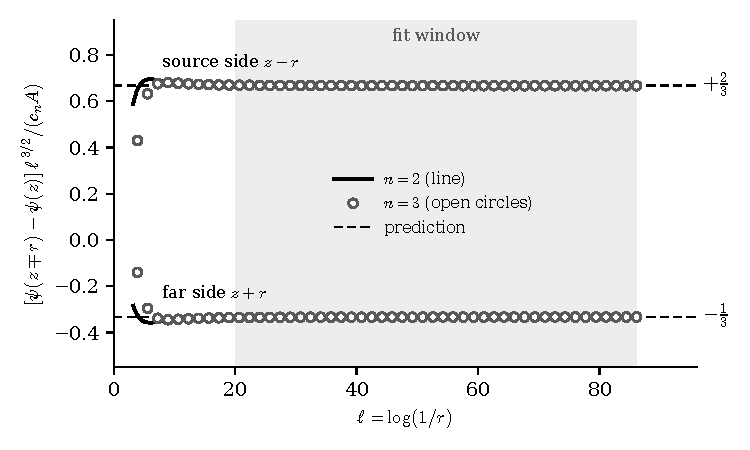
\includegraphics[width=0.62\textwidth]{numerics/fig_kink_split.pdf}
\caption{Generation-$1$ kink profile at $L=0.6$ (even ground state for $s=0$, $\lambda=-2.417$, $A=1.567$; P1, grading $\rho=1.15$ down to $r=10^{-40}$; registered run). Plotted: the one-sided excursions $[\psi(z\mp r)-\psi(z)]\ell^{3/2}/(c_nA)$ at $z=y_n$, with $\psi(z)$ from the cusp fit. Dashed: the predicted values $+\frac23$ (source side) and $-\frac13$ (far side) of Theorem~\ref{thm:kink}. Line: $n=2$; circles: $n=3$ (every $12$th node). The two coincide because $D\approx-0.002$ and $\beta_2=\beta_3=0$ here, so the $O(1/\ell)$ correction nearly vanishes. Fitted limits: $0.66679$ and $-0.33335$ at both points.}\label{fig:kink}
\end{figure}

\subsection{Tail law}
\emph{Registered.} The tail tests use P1 eigenfunctions and the $10\,500$ zeros up to height $T=10\,303$. The states are the ground states of their sector for pole weights $s=-1,0,5,20$, chosen with large $|\lambda|$ so that the $\lambda$-dependence is visible; they therefore test the theorems where $\lambda/\log T$ is large, not the true form at small $\lambda$. We compare the zero-side block sums $Z$ over seven blocks between $T=100$ and $T=10\,300$ with $Z_{\rm pred}=\frac{|\lambda'|}\pi\int\frac{a+\eps c_X}{t^2(a-\lambda)}$ over the block, i.e.\ with the main term of Proposition~\ref{prop:T4}, where $2A^2$ is replaced by $|\lambda'|$. That replacement uses Theorem~\ref{thm:H} and hence sector-simplicity. For the even states ($s=-1,0$) this is Proposition~\ref{prop:nonvan}(a); for the odd states ($s=5,20$) it is observed numerically and assumed, not proved. $Z/Z_{\rm pred}$ rises from $0.80$--$0.98$ on $[100,200]$ to $0.968$--$1.000$ on $[6400,10300]$; without the $\lambda$-shift in the denominator the ratio is $0.20$--$0.87$. The registered tolerance was generous ($2\sum_{n<X}c_n^2\langle a^{-2}\rangle+0.005$, i.e.\ $0.13$--$0.21$ on $[400,800]$), and all graded states passed inside it by a factor of at least $2$; this test sees the $\lambda$-shift but would not see a constant error below about $10\%$ at $T\le10^4$. The first-order law $\pi TZ\to|\lambda'|$ itself is not testable at these heights ($\Upsilon(6400)=0.42$--$0.88$ for these states), and Theorem~\ref{thm:T5} was not tested.

\emph{The term $\eps c_X$.} It is cleanest at $X=2,3$, where no product $nm=X$ competes. \emph{Not registered:} for P0 eigenfunctions ($s=0,1$ at $X=2$, $s=0$ at $X=3$; zeros $1$--$1500$, three blocks in $[250,1981]$) the ratio of the zero-side block sums to the prediction is $0.968$--$1.014$ with the term and $1.09$--$1.13$ (even) and $0.86$--$0.91$ (odd) without it, so the sector sign is right; the control $L=0.4$ ($c_X=0$) gives $0.971$--$0.999$. Here sector-simplicity is proved (Proposition~\ref{prop:nonvan}, Remark~\ref{rem:simple}) except for the odd state at $X=3$, where it is assumed. At $X=4$ (even sector, $s=0$, $T\in[100,1600]$) the ratios are $0.989$--$0.994$ with the term and $1.06$--$1.10$ without it. A direct check of the sign of Landau's term on the zeros ($\sum_{0<t_\rho\le T}\cos(t_\rho\log X)$ against $-\frac T{2\pi}c_X$ for $X=2,3,4,8$, with controls $X=6,10$) agrees to within $0.5\%$ at $T=10\,303$. \emph{Registered:} at $X=8$ we fit, over six blocks $k$, $\ln(Z_e/E_e)_k-\ln(Z_o/E_o)_k=\alpha\langle1/a\rangle_k+\alpha_2\langle a^{-2}\rangle_k$, where $E$ is the smooth analogue $\frac1\pi\int_{\rm block}a|F|^2$, with prediction $\alpha=2c_X$ and pass rule $|\alpha-2c_X|\le\max(0.10,3\sigma_\alpha)$. This gives $\alpha=0.51$--$0.67$ against $2c_8=0.490$; two of the four pairs are high by $2.6\sigma$ and $3.0\sigma$, the second passing the registered $3\sigma$ rule by less than $0.003$. The control $X=6$ gives $\alpha=0.02\pm0.07$; the control $X=10$ ($0.32$--$0.44\pm0.19$) is uninformative. The $c_X$ term is supported at $X=2,3,4,8$ but not established; at $X=8$ it is not cleanly separated from the $\ell^{-2}$ terms discussed in Section~\ref{sec:conj}.

\subsection{Limits}
Kink tests need $|A|\gtrsim0.2$. The true-form ground states at $L\ge0.6$ ($A_e\lesssim3\e{-4}$, Section~\ref{sec:status}) are beyond what these double-precision tests resolve and were not tested, and neither was Conjecture~\ref{conj:K7}. All codes are uncertified.

% =====================================================================
\section{Conjectures and open problems}\label{sec:conj}

Conjecture~\ref{conj:K7} (the second-order even part of the kink law) is stated in Section~\ref{sec:kink}. The following statements are open.

\begin{conjecture}[sharp per-sector law]\label{conj:L}
At fixed $L$, $\pi T\,Z_\times(T)=O_\psi(\log^{-3/2}T)$, with a constant that may depend on $\delta_X$, and likewise for the smooth analogue $E_\times$.
\end{conjecture}

A heuristic based on the kink law suggests $O(\log^{-2}T)$. The conjecture cannot hold uniformly as $L$ decreases to an activation point: for $n<X$ with small $\Delta_n=2L-\log n$, the edge-times-opposite-kink term against the smooth density is of order $c_n\min(1,(T\Delta_n)^{-1})/\ell_T$. Under Conjecture~\ref{conj:L}, for sector-simple states with $A\ne0$, $\Upsilon(T)=T\int_T^\infty\frac{a+\eps c_X}{t^2(a-\lambda)}\dd t+O(\ell_T^{-3/2})$, and for the two parity ground states the derivative-free split $\ln\frac{Z_e}{E_e}-\ln\frac{Z_o}{E_o}=\frac{2c_X}{a(T)}+O(\ell_T^{-3/2})$ would follow.

\begin{conjecture}[refined smoothed law]\label{conj:R}
For $A\ne0$, $\frac{Z_{\cos}(z)}{A^2z}-1=\frac{\lambda+\eps c_X}{\ell-D+1}+\frac{\kappa_{\rm kink}}{\ell^2}+O(\ell^{-3})$, with a constant $\kappa_{\rm kink}$ depending on $L$ and the sector, to be derived from the kink law.
\end{conjecture}

The form with $\kappa_{\rm kink}=0$ is probably false when $e^{2L}=nm$ (a sector term $\pm2\sum_{nm=X}c_nc_m$ is expected) and plausibly whenever a prime power $n<X$ is active. The $c_X$ part is proved (Theorem~\ref{thm:contact}), and so is the order $1/\ell$ of everything (Theorem~\ref{thm:T3}).

\begin{conjecture}[sharp refined law]\label{pred:F}
For a sector-simple $\lambda_\sigma$ with $A\ne0$, $\Upsilon_\sigma(T):=\frac{\pi TZ(T)}{|\lambda_\sigma'|}=1+\frac{\lambda_\sigma+\eps_\sigma c_X}{\log(T/2\pi)+1-\lambda_\sigma}+o\bigl(\frac1{\log T}\bigr)$.
\end{conjecture}

By Proposition~\ref{prop:T6}(c), Conjecture~\ref{pred:F} is equivalent to $\pi TZ_\times(T)=o(1/\log T)$, which Conjecture~\ref{conj:L} implies. The zero-side tests of Section~\ref{sec:numerics} are consistent with it.

\emph{Where the $\ell^{-2}$ terms come from (heuristic).} Edge-times-kink cross terms in the zero sum resonate with the prime part of the zero density at the frequencies $\log n$ (Landau's formula at $x=n$); by Theorem~\ref{thm:kink} the kink at $y_n$ has Fourier amplitude about $c_n/\log t$ relative to the edge. This suggests a sector-independent term $-\kappa\sum_{n<X}c_n^2/\ell^2$ in $Z$, with $\kappa\approx\frac12$ in the P1 data, and a sector term $\pm2\sum_{nm=X}c_nc_m/\ell^2$; deriving them from Theorems~\ref{thm:kink} and~\ref{thm:K5} (with asymptotics of the type of~\cite{WL78}) is a natural next step.

\begin{conjecture}[$A_e\ne0$]\label{conj:Ae}
For the true form ($s=1$) and every $L\in(0,1.19]$, the even ground state has $A_e(L)\ne0$.
\end{conjecture}

\emph{What is proved about Conjecture~\ref{conj:Ae}.} (i) By Theorem~\ref{thm:transl}(d) (\cite[(6.3)]{BT26}, \cite{SoDa}), at a crossing of an even and an odd level, $A_eA_o=0$. (ii) By Proposition~\ref{prop:nonvan}(b), for $2L\le\log2$ the odd ground state has $A_o>0$; so if, along $s\mapsto H^{(s)}_L$, the lowest even level meets the lowest odd level at some $s_{\rm up}$ where both are sector-simple, the even state has $A_e=0$ there. (iii) By Proposition~\ref{prop:nonvan}(c), on $(0,1.19)$ the set where $A_e=0$ is closed and nowhere dense, given~\cite{GS}.

\emph{Relation to simple-even.} On the even sector the pole is the rank-one form $2s(\int f\cosh\frac x2)^2$, so by the Aronszajn--Krein formula, whenever $\lambda_e(s)$ is not an eigenvalue of $H^{(0)}_e$, $A_e(s)$ is proportional to $\alpha_{\rm res}(\lambda_e(s))$, where $\alpha_{\rm res}(\lambda)$ is the edge trace of $(H^{(0)}_e-\lambda)^{-1}\cosh\frac x2$ and $H^{(0)}_e$ is the even part of the pole-free operator. In this picture ``simple-even at $s=1$'' corresponds to ``$A_e(s)\ne0$ for $s\in[0,1]$''. This correspondence is \emph{not} a theorem. The direction ``a crossing below $s=1$ forces $A_e(s_{\rm up})=0$'' needs sector-simplicity at $s_{\rm up}$ and $A_o(s_{\rm up})\neq0$; the latter is known only for $2L\le\log2$, and in our (hp-FEM) computations the odd edge value at $s_{\rm up}$ changes sign between $L=0.4$ and $L=0.6$, so it cannot simply be assumed. The converse needs the absence of an interior node of the even branch for $s<s_{\rm up}$, which we cannot prove. Modulo these hypotheses, Conjecture~\ref{conj:Ae} is the same hard core as the simple-even property, and as the open question left by the rank-one (Herglotz) reduction of even-simplicity in~\cite{And3} (see also the parity rank-one pole and Herglotz criterion in~\cite{Oen}).

\emph{Further open problems.} (1) Uniformity in $L$ near the activation points $2L=\log n$, and over the dense set $C_L$. (2) $C^\infty$ smoothness off $\overline{C_L}$, third-order terms, edge asymptotics of $\psi'$, and whether $\psi\in BV$. (3) The sign of $A_+(\psi_e)A_+(\psi_o)$ under a natural normalisation. (4) Other $L$-functions: Theorems~\ref{thm:K1}, \ref{thm:kink} and~\ref{thm:K5} use only that the $c_n$ are real, but weights of chains of equal length may cancel, and $D$ changes with the archimedean constants.

% =====================================================================
\section{Scope}\label{sec:scope}
As stated in Section~\ref{sec:status}, this paper studies a quadratic form, and none of its results proves or disproves the Riemann hypothesis; where zeta zeros enter, no hypothesis on their location is made. We add three points. The constants in the asymptotic laws (for instance $\mathsf B$ in Theorem~\ref{thm:T1} and the pointwise constants of Sections~\ref{sec:interior}--\ref{sec:kink}) are not computed and are not uniform in $L$ near the activation points. The paper proves no new simplicity of an eigenvalue of the true form; the input~\cite{GS} is used on $(0,1.19]$ only. It gives no positivity of $Q_L$ at any $L$.

% =====================================================================
\section*{Credits}
Section~\ref{sec:novelty} gives the attributions in detail; we summarise them here. The existence of the edge traces, a limit formula for them, the Hadamard formula with $|A_+|=|A_-|$ and rank at most one, the activation formula for eigenvalues, and the pure-log trace identity with simplicity are due to the rStation agent bramble\_trace~\cite{BT26,BT26a,BT26b}. The mathia notes of S.~Garcia Murillo derived the trace with a remainder $O(\ell^{-1})$ in substance~\cite{PL319,PL323,PL329,PL336,PL337,PL338}, posed the zero-order Hadamard question and reduced it to conditional statements~\cite{mathiaClue,PL297,PL305,PL306,PL307}, found the prime-activation mechanism behind our $c_X$ contact term~\cite{PL338}, and contain the Beurling--Deny thresholds of Proposition~\ref{prop:nonvan}~\cite{PL294,PL324,PL335} and, for $s=1$ at $2L=\log2$, the positivity $A_o>0$~\cite{PL335}; commit identifiers are given in the references. The locations of the weak singular points, $\pm(L-\log n)$ in our convention, were found by L.~Eberwein \cite[\S13, p.~45]{Eb}. A heuristic fit containing the offset $D$ was posted by span\_of\_dilates~\cite{SoDb}. The explicit L\'evy kernel $J$ and the Dirichlet-form reading of the archimedean term are in~\cite{Suz26,And1,Oen,BT26}. Joubert~\cite{Jou} related the lowest eigenvalue numerically to the squared edge value through zero-side leakage, and Kim et al.~\cite{Kim26} posed the boundary exponent as an open problem. The Wiener--Hopf tools are Kwa\'snicki's~\cite{Kw11}. The simplicity input~\cite{GS} rests on the frequency-cutoff reduction of Zhu~\cite{Zhu}. Several lemmas were contributed by AI referee passes within this project (see below).

\section*{Verification status and AI assistance}
The arguments, the code and the text were developed with substantial assistance from an AI system (Anthropic's Claude), directed by the author. All checking so far has been AI-assisted: each proof went through repeated AI referee passes before this text was assembled (Theorems~\ref{thm:T3} and~\ref{thm:T5} and Proposition~\ref{prop:T6} only once), and the assembled text went through further passes on the proofs, on novelty and citations, and on exposition. The last proof pass found no mathematical error in any statement labelled as proved, found no use of RH, and recomputed the numerical constants with independent code. Several ingredients came from these passes: the renewal asymptotics (R1)--(R2) and a jump lemma, the sliding-window density argument in Corollary~\ref{cor:K4}(c), the even-part outline behind Conjecture~\ref{conj:K7}, the canonical main term $\Phi_c$ of Theorem~\ref{thm:T1}, and the two-pass bootstrap in its proof. The revisions made after the last pass (the comparison with~\cite{BT26} and the mathia notes, the exact main term in Lemmas~\ref{lem:field} and~\ref{lem:layer}, the ranges in Lemma~\ref{lem:Z} and Proposition~\ref{prop:T4}, and the uniformity statement of Theorem~\ref{thm:K1}(a)) were checked only by the second review described next. \emph{Second review.} On 31 October 2026 the assembled text, with all appendices and the supplied numerical files, was reviewed by a separate AI system (OpenAI's Codex, model GPT-6.1 Sol, high reasoning effort), which recommended release as a preprint after minor fixes and found no fatal or major mathematical error in the principal results. It checked the normalisations and the operator set-up of Section~\ref{sec:setting} (with a numerical check of the L\'evy representation of $\Psi_a$), the half-line inversion and the first edge law (Sections~\ref{sec:WH}--\ref{sec:edge}, Appendix~\ref{app:Linf}), the cross identity, the layer integral and the factors in Section~\ref{sec:H}, the renewal constants and the kink coefficients of Sections~\ref{sec:interior}--\ref{sec:kink} (with an independent quadrature of the free resolvent at $q=1$, not error-certified), the transfer matrix, the generation induction and every entry of Table~\ref{tab:boosts}, the zero-side arguments of Sections~\ref{sec:zero1}--\ref{sec:zero2} and Appendices~\ref{app:T1}--\ref{app:T2} (finding no hidden use of RH), and the Mellin constants of Proposition~\ref{prop:T6}; it reran the supplied numerical analysis (checksums, verdicts, and an independent refit, which reproduced the odd-state failure of the rerun), inspected the cited rStation statements and posting dates of~\cite{BT26,BT26a,BT26b}, checked the cited theorem numbers and hypotheses of~\cite{Kw11,Suz26,KW26,Den06,BK17}, and repeated the novelty searches. It did not check~\cite{GS}, the large Galerkin solves, the unsupplied original P0, hp and tail runs, or every bibliography entry. Its findings were addressed in this version: the normalisation of the heuristic in Section~\ref{sec:strategy} and Remark~\ref{rem:T0}, the qualification of the reciprocal-moment expansion in the proof of Proposition~\ref{prop:T6}(b), the disclosure and check of the anchor rule of P1 (Section~\ref{sec:numerics}), the order of magnitude previously stated for $A_e$ at larger $L$ (Section~\ref{sec:status}), and the length of the priority material in the abstract; the completeness of the numerical supplement is addressed in the supplementary files. These changes have not been reviewed again. \emph{No human expert has yet checked the proofs or the code.} The parts that most need an expert reading are: Step~4 of Lemma~\ref{lem:WH} (the Hardy-space step); the $L^\infty$ bound (Appendix~\ref{app:Linf}); Lemma~\ref{lem:cont}; Lemmas~\ref{lem:field} and~\ref{lem:layer}, with Lemmas~\ref{lem:Klevy} and~\ref{lem:extid}, which fix the constant in Theorem~\ref{thm:H}; the edge transform (Lemma~\ref{lem:edgeT}); and the zero-side estimates (Lemma~\ref{lem:Z}, Landau's formula with zeros off the line, the pairing $\rho\mapsto1-\bar\rho$). Theorem numbers of~\cite{Kw11} refer to arXiv:1006.0524v4; those of \cite[Thms.~5.2, 6.2]{SSV12} and \cite[Thm.~VI.20]{Bertoin96} were not checked against the books; equation~(43) of~\cite{BK17} is numbered as in arXiv:1012.3881v3; the description of~\cite{KW26} is taken from the author's reading for~\cite{BPL} and was checked by the second review; and of~\cite{VS23,VS26} only the abstract of~\cite{VS23} was read. The simplicity input~\cite{GS} is computer-assisted and unrefereed. The author takes full responsibility for the content.

\section*{Data availability}
The numerical supplement of this paper (\texttt{supplement.zip}, about 17~MB) contains what is needed to reproduce Section~\ref{sec:numerics}: the P1 solver and the kink and tail scripts with both registration files and their checksums; the $10\,500$ zeta zeros; the raw output of every P1 run (the registered kink and tail runs, the post-registration $L=1.0$ diagnostic and the registered rerun); the scripts that compute the error bands and generate Tables~\ref{tab:kink1}--\ref{tab:k0}, the data of Table~\ref{tab:k5} and Figure~\ref{fig:kink}; the check of the anchor rule described under Methods; and, for the unregistered checks, the P0 and hp-FEM codes with the outputs behind Table~\ref{tab:H} and the zero-side computations at $X=2,3,4$. Its README gives the software versions, the command and the input files for each table and the figure, and the run times. From a fresh extraction the tables and the figure were regenerated from the stored raw output and agree with the printed ones, and a script in the supplement recomputes the numbers quoted in Section~\ref{sec:numerics} from the stored output. All registered kink runs and the diagnostic were also repeated, and the tables regenerated from the new output are identical. The tail runs and the two finer meshes of the rerun were not repeated; shorter runs of the tail, P0 and hp-FEM codes were, and reproduced the stored output. Not in the supplement: the code behind the fit-model comparison and the flatness diagnostic in the paragraph on the second-order edge law, which was run during the last internal review and not kept, so those numbers cannot be reproduced from it.

\emph{Registration record.} The P1 kink and tail tests were registered on 31 October 2026, before any run, in a file that fixes the tests, the pass rules and the tolerances and records the checksums of all scripts; the $L=1.0$ rerun was registered separately, before its batch started. After the first registration the analysis script was corrected in one respect: the two sides of a measured point are matched by common offsets rather than by prefix. The registered version stops with an error on one of the two runs with mirror points ($\rho=1.25$) and on two of the three $L=0.8$ runs; on every other run its output is identical to that of the corrected version (both versions are in the supplement). In the rerun the summary step was repeated with unchanged, checksum-verified code after a parsing failure. The error bands were computed after the runs. The registration files use route labels: K0$'$ is Theorem~\ref{thm:K1}(c), K1 and K2 are Theorem~\ref{thm:kink} with $k=1,2$, K5 is Corollary~\ref{cor:K6}(a), and T1, T2 are the tail and sector-split tests of Section~\ref{sec:numerics}. These files, with their checksums and time stamps, are in the supplement. In two of them (the registration file and the batch script of the rerun) the name of the computer and its working folders were replaced by placeholders before release, so these two no longer match their registered checksums; the README lists every replaced string. All other registered checksums match, except that of the analysis script, whose registered version is included separately and matches.

\section*{Competing interests}
The author declares no competing interests.

\section*{Funding}
This work received no external funding.

% =====================================================================
\appendix
\section{Proof of Lemma~\ref{lem:Linf} (boundedness)}\label{app:Linf}

Let $I=(-L,L)$. Let $\mathcal A$ be the self-adjoint operator of $(\cE,\mathcal D(\cE))$ on $L^2(\R)$, i.e.\ the Fourier multiplier $\Psi_a$, and $A_D$ the self-adjoint operator of the closed nonnegative form $(\cE,\mathcal D_L)$ on $L^2(I)$ \cite[Thm.~VI.2.1]{Kato95}: $u\in \mathcal D(A_D)$ and $A_Du=g$ iff $u\in \mathcal D_L$ and $\cE(u,\phi)=\langle g,\phi\rangle$ for all $\phi\in \mathcal D_L$. Let $P(t)=e^{-t\mathcal A}$ and $S(t)=e^{-tA_D}$.

\emph{Step 1: the free kernel.} Since $\varphi$ is a Bernstein function with $\varphi(0+)=0$, there is a convolution semigroup of probability measures $(\eta_t)_{t\ge0}$ on $[0,\infty)$ with $\int e^{-ur}\eta_t(\dd r)=e^{-t\varphi(u)}$ \cite[Thm.~5.2]{SSV12}; as $\varphi(\infty)=\infty$, $\eta_t(\{0\})=0$ for $t>0$. With $g_r(x)=(4\pi r)^{-1/2}e^{-x^2/4r}$, $\hat g_r(\xi)=e^{-r\xi^2}$, put $p_t=\int g_r\,\eta_t(\dd r)$. Then $p_t\ge0$, $\int p_t=1$, $\hat p_t=e^{-t\Psi_a}$ and $P(t)g=p_t*g$. For $1<m\le\infty$ and $\alpha=\frac12(1-\frac1m)$, $\|g_r\|_m\le r^{-\alpha}$, and $r^{-\alpha}=\Gamma(\alpha)^{-1}\int_0^\infty u^{\alpha-1}e^{-ur}\dd u$ gives
\[
\|p_t\|_m\le\int r^{-\alpha}\eta_t(\dd r)=\frac1{\Gamma(\alpha)}\int_0^\infty u^{\alpha-1}e^{-t\varphi(u)}\dd u\le\frac1{\Gamma(\alpha)}\Bigl[\frac1\alpha+e^{tC_\varphi}\int_1^\infty u^{\alpha-1-t/2}\dd u\Bigr],
\]
using $\varphi(u)\ge\frac12\log u-C_\varphi$ for $u\ge1$ (Lemma~\ref{lem:symbol}(c)). Hence
\begin{equation}\label{eq:pt}
\|p_t\|_m<\infty\qquad\text{whenever}\qquad1-\tfrac1m<t,
\end{equation}
with a bound depending only on $t$ and $m$.

\emph{Step 2: domination.} We claim $|S(t)g|\le P(t)|g|$ a.e.\ on $I$ for real $g\in L^2(I)$, extended by zero. Let $q>0$, $g\ge0$, $u_D=(A_D+q)^{-1}g\in \mathcal D_L$ and $u=r_q*g\ge0$, so that $\cE_q(u_D,\phi)=\langle g,\phi\rangle$ for $\phi\in \mathcal D_L$ and $\cE_q(u,\phi)=\langle g,\phi\rangle$ for $\phi\in \mathcal D(\cE)$. By Lemma~\ref{lem:DF}(b),(c), $u_D^-\in \mathcal D_L$ and $0\le\langle g,u_D^-\rangle=\cE_q(u_D,u_D^-)\le-q\|u_D^-\|^2$, so $u_D\ge0$. Let $F=u_D-u$; off $I$, $F=-u\le0$, so $F^+\in \mathcal D_L$, and subtracting the two equations tested with $F^+$ gives $0=\cE_q(F,F^+)\ge q\|F^+\|^2$, so $u_D\le u$. With $R_D=(A_D+q)^{-1}$ and $R=(\mathcal A+q)^{-1}$, both positivity preserving, induction gives $R_D^ng\le\one_IR^ng$. Taking $q=n/t$, $(1+\frac tnA_D)^{-n}\to S(t)$ and $(1+\frac tn\mathcal A)^{-n}\to P(t)$ strongly by the spectral theorem; along a subsequence the convergence is a.e., so $0\le S(t)g\le P(t)g$ on $I$. For real $g$ split $g=g^+-g^-$. By Young's inequality, for $2\le p\le r\le\infty$ and $1+\frac1r=\frac1m+\frac1p$,
\begin{equation}\label{eq:smooth}
\|S(t)g\|_{L^r(I)}\le\|p_t\|_m\|g\|_{L^p(I)},\qquad\text{in particular}\quad\|S(t)\|_{r\to r}\le1 .
\end{equation}

\emph{Step 3: Duhamel.} For $\phi\in \mathcal D_L$, $\cE(\psi,\phi)=\langle\lambda\psi-W_L\psi,\phi\rangle$ with $W_L=\one_IW_s\one_I$, so $\psi\in \mathcal D(A_D)$ and $A_D\psi=\lambda\psi-W_L\psi$, and $\|W_L\|_{r\to r}\le M$ for $1\le r\le\infty$ (Lemma~\ref{lem:window}). The map $t'\mapsto e^{t'\lambda}S(t')\psi$ is $C^1$ in $L^2(I)$ with derivative $e^{t'\lambda}S(t')W_L\psi$; integrating over $[0,\tau]$,
\[
e^{\tau\lambda}S(\tau)\psi=(1+T_\tau)\psi,\qquad T_\tau g:=\int_0^\tau e^{t'\lambda}S(t')W_Lg\dd t' .
\]
For $2\le r\le\infty$, $g\in L^r(I)$ and $h\in L^2(I)$, $|\langle T_\tau g,h\rangle|\le\tau e^{\tau\Lambda_0}M\|g\|_r\|h\|_{r'}$ by~\eqref{eq:smooth}; since $L^2(I)$ is dense in $L^{r'}(I)$, $\|T_\tau\|_{r\to r}\le\tau e^{\tau\Lambda_0}M$. Fix $\tau\in(0,1]$ with $\tau e^{\tau\Lambda_0}M\le\frac12$. The Neumann series inverts $1+T_\tau$ on every $L^r(I)$, $2\le r\le\infty$, with norm at most $2$, consistently with $L^2(I)$ since $I$ is bounded.

\emph{Step 4: bootstrap.} Let $\frac1{p_0}=\frac12$ and $\frac1{p_{k+1}}=\max(\frac1{p_k}-\frac\tau2,0)$, so $p_K=\infty$ for $K=\lceil1/\tau\rceil$. With $\frac1{m_k}=1-(\frac1{p_k}-\frac1{p_{k+1}})$ we have $1-\frac1{m_k}\le\frac\tau2<\tau$, so $\|p_\tau\|_{m_k}\le C$ by~\eqref{eq:pt}. From $\psi=(1+T_\tau)^{-1}e^{\tau\lambda}S(\tau)\psi$ and~\eqref{eq:smooth}, $\|\psi\|_{p_{k+1}}\le2e^{\tau\Lambda_0}C\|\psi\|_{p_k}$. After $K$ steps $\|\psi\|_\infty\le C_\infty\|\psi\|_2$, with $C_\infty$ depending only on $\Lambda_0$, $M$ and $C_\varphi$, hence only on $L_{\max}$, $S_0$ and $\Lambda_0$.
\qed

% =====================================================================
\section{Proof of Theorem~\ref{thm:T1} (Fourier edge law)}\label{app:T1}

Throughout, $L$, $s$ and $\Lambda_0$ are fixed, $|\lambda|\le\Lambda_0$, and constants depend on $(L,s,\Lambda_0)$ and on fixed cutoffs; they are uniform over eigenfunctions and do not involve $A_\pm$. Put $u=u_+=\chi\tilde\psi=G_qf_+$ (Theorem~\ref{thm:E}(iv)), $A=A_+$, $W'=W_s-c$, and $g'=H\bigl[r_\chi[\tilde\psi]-\chi W'\tilde\psi\bigr]$, so that $f_+=\mu_qu+g'$. Let $\hat r_{q,-}(t)=\int_{-\infty}^0r_q(z)e^{izt}\dd z$ and $\delta_L=\min(\rho_0/2,\delta_X/2)$.

\begin{lemma}[$K$ on the imaginary axis]\label{lem:Kaxis}
Write $K(z)=\sqrt q+\int\frac z{z+\tau}\Theta(\dd\tau)$ \cite[Thm.~6.2]{SSV12}; the linear coefficient vanishes because $K(\xi)^2\sim\log\xi$ (Lemma~\ref{lem:Kasym}). For $t>0$: (a) $t|K'(it)|\le\im K(it)\le|K(it)|$; (b) $0\le\arg K(it)\le C/\ell_t$ for $t\ge2$.
\end{lemma}

\begin{proof}
$\re K(it)=\sqrt q+\int\frac{t^2}{t^2+\tau^2}\Theta\ge0$ and $\im K(it)=\int\frac{t\tau}{t^2+\tau^2}\Theta\ge0$. (a) $|K'(it)|\le\int\frac\tau{t^2+\tau^2}\Theta$. (b) $tK'(t)=\int\frac{t\tau}{(t+\tau)^2}\Theta$ and $(t+\tau)^2\le2(t^2+\tau^2)$ give $\im K(it)\le2\beta(t)K(t)$; with $K(t)\le C|K(it)|$ (Lemma~\ref{lem:Kasym}(a) and (K3)) and $\beta(t)\le C/\ell_t$, $\sin\arg K(it)\le C/\ell_t$, and $\arg K(it)\in[0,\frac\pi2]$.
\end{proof}

\begin{lemma}[second-order half-line edge transform]\label{lem:edgeT}
Let $U(t)=K(it)(1-\mu_q\hat r_{q,-}(t))$, $t\in\R$; then $U(-t)=\overline{U(t)}$. For $|t|\ge t_0$,
\begin{equation}\label{eq:edgeT}
(a(t)-\lambda)\,\hat u(t)=-\frac{A\,U(t)}{it}+\widehat{g_0}(t)+\mathcal R(t),
\end{equation}
where $g_0=Hw$ with $w\in L^2\cap L^\infty$ given in~\eqref{eq:w}, $w$ continuous at $0$ with $w(0)=0$ and $|w(y)|\le C/\ell(|y|)$ for $|y|\le\delta_L$, and $|\mathcal R(t)|\le C/(|t|\ell_{|t|})$. Moreover $|U|^2=a-\lambda+\mu_q^2\sigma_q|\hat r_{q,-}|^2$ exactly, $\re\hat r_{q,-}=\frac1{2\sigma_q}$ and $|\im\hat r_{q,-}(t)|\le C/\ell_t$; hence $|U|^2=(a-\lambda)(1+O(\ell_t^{-2}))$, $|U'(t)|\le C\ell_t^{1/2}/t$, and $\theta_U:=\arg U=O(1/\ell_t)$. The same holds at $-L$ with $A_-$.
\end{lemma}

\begin{proof}
\emph{Exact equation.} By~\eqref{eq:WH}, $\sigma_q\hat u=\hat f_+-K(it)\widehat{P_-k_+}$ with $k_+=\tilde v*f_+$; subtracting $\mu_q\hat u$ and using $\sigma_q-\mu_q=a-\lambda$,
\[
(a-\lambda)\hat u=\widehat{g'}-K(it)\widehat{P_-k_+},\qquad k_+(0)=\int vf_+=A .
\]
\emph{$g'$ near $0$.} For $0<y<\rho_0$: $r_\chi[\tilde\psi]$ and $P_s\tilde\psi$ are smooth; $S_n^*\tilde\psi(y)=0$ for $y<\log n$; $S_n\tilde\psi(y)=\psi(y_n-y)$, which vanishes for $y<\log n-2L$ if $\log n>2L$, equals $\psi(-L-y)=0$ if $n=X$, and is an interior value if $\log n<2L$. So $g'(0):=g'(0+)$ exists and $|g'(y)-g'(0)|\le C/\ell(y)$ on $(0,\delta_L]$ (Lemma~\ref{lem:modulus}(a$'$)).
\emph{Splitting $k_+$ on $(-\infty,0)$.} Let $f_r=f_+-\mu_qAV$ on $(0,\infty)$. Since $V=v*H$ and $r_q=v*\tilde v$, $\tilde v*(HV)=r_q*H=:R_q$, $R_q(z)=\int_{-\infty}^zr_q$, $R_q(0)=\frac1{2q}$. For $z<0$, $k_+(z)=\mu_qAR_q(z)+k_r(-z)$ with $k_r(s)=\int_0^\infty v(y+s)f_r(y)\dd y$ and $k_r(0)=A(1-\frac{\mu_q}{2q})$ (as $\int_0^\infty vV=\frac1{2q}$). The first piece is integrable on $(-\infty,0)$ (Lemma~\ref{lem:rq}(b)) and $\int_{-\infty}^0R_q(z)e^{izt}\dd z=\frac1{it}(\frac1{2q}-\hat r_{q,-}(t))$. For the second, $f_r=\mu_q(\tilde\psi-AV)+g'$ on $(0,\rho_0]$, so $\eps_r:=f_r-g'(0)$ is bounded with $|\eps_r(y)|\le C/\ell(y)$ on $(0,\delta_L]$. Then $k_r'(s)=-g'(0)v(s)-d(s)$ with $d(s)=\int_0^\infty(-v')(y+s)\eps_r(y)\dd y$. ($k_r$ is bounded and integrable: $\int_0^\infty sv(s)\dd s=K'(0+)/q<\infty$, since $\frac{K'}K(\xi)=\frac1\pi\int_0^\infty\frac{\tau\sigma_q'(\xi\tau)}{\sigma_q(\xi\tau)}\frac{\dd\tau}{1+\tau^2}$ is bounded as $\xi\downarrow0$ because $\sigma_q'(x)\le C\min(x,1/x)$.) Integrating by parts and using $\int_0^\infty ve^{-ist}\dd s=1/K(it)$,
\[
\int_0^\infty k_r(s)e^{-ist}\dd s=\frac1{it}\Bigl[k_r(0)-\frac{g'(0)}{K(it)}-\hat d(t)\Bigr],\qquad\hat d(t)=\int_0^\infty d(s)e^{-ist}\dd s .
\]
Since $\frac{\mu_qA}{2q}+k_r(0)=A$, this gives $K(it)\widehat{P_-k_+}=\frac1{it}[AU(t)-g'(0)-K(it)\hat d(t)]$.
\emph{The jump cancels.} With $\zeta\in C_c^\infty$, $\zeta=1$ on $[-\delta_L,\delta_L]$, define
\begin{equation}\label{eq:w}
w=r_\chi[\tilde\psi]-\chi P_s\tilde\psi+\chi\sum_{n\ne X}c_n(S_n+S_n^*)\tilde\psi-g'(0)\zeta\qquad(\text{the shift by }\log X\text{ omitted}).
\end{equation}
For $y>0$, $S_X\tilde\psi(y)=\psi(-L-y)=0$ and $\chi(y)S_X^*\tilde\psi(y)=\chi(y)\psi(3L-y)=0$, so $Hw=g'-g'(0)\zeta H=:g_0$. The function $w$ is continuous at $0$ with $w(0)=0$ and $|w(y)|\le C/\ell(|y|)$ on both sides. (Omitting $n=X$ is necessary: for $y<0$ that shift would contribute $c_X\psi(-L+|y|)\sim c_XA_-\ell^{-1/2}$.) As $\widehat{\zeta H}(t)=-\frac1{it}+O(t^{-N})$, $\widehat{g'}=\widehat{g_0}-\frac{g'(0)}{it}+O(t^{-N})$; the $g'(0)$ terms cancel and~\eqref{eq:edgeT} holds with $\mathcal R=\frac{K(it)\hat d(t)}{it}+O(t^{-N})$.
\emph{Bounds on $d$.} For $0<s\le\delta_L/2$ split $d(s)$ at $y=s$ and $y=\delta_L$. For $y<s$, $(-v')(y+s)\le2v(s/2)/s$ against $\int_0^s|\eps_r|\le Cs/\ell(s)$. For $s<y<\delta_L$, $(-v')(y+s)\le(-v')(y)$ and $\int_s^{\delta_L}\frac{(-v')(y)}{\ell(y)}\dd y\le\frac{v(s)}{\ell(s)}+\int_s^{\delta_L}\frac{v(y)}{y\ell(y)^2}\dd y$. For $y>\delta_L$ the contribution is $\le Cv(\delta_L)$. With Lemma~\ref{lem:rq}(e),(f), $|d(s)|\le C/(s\ell(s)^{5/2})$, and in the same way ($v''$ is decreasing) $|d'(s)|\le C/(s^2\ell(s)^{5/2})$; for $s>\delta_L/2$, $|d|\le Cv(s)$ and $|d'|\le C|v'(s)|$. Then, for $t\ge2$, $|\hat d(t)|\le\int_0^{1/t}|d|+\frac1t\bigl(|d(1/t)|+\int_{1/t}^\infty|d'|\bigr)\le C\ell_t^{-3/2}$, since $\int_0^x\frac{\dd s}{s\ell(s)^{5/2}}=\frac23\ell(x)^{-3/2}$; with $|K(it)|=\sigma_q^{1/2}\le C\ell_t^{1/2}$, $|\mathcal R|\le C/(t\ell_t)$.
\emph{$|U|^2$.} Since $r_q$ is even, $\hat r_{q,-}+\overline{\hat r_{q,-}}=\hat r_q=1/\sigma_q$, so $|U|^2=\sigma_q(1-2\mu_q\re\hat r_{q,-}+\mu_q^2|\hat r_{q,-}|^2)=\sigma_q-\mu_q+\mu_q^2\sigma_q|\hat r_{q,-}|^2$. By the second mean value theorem, $|\im\hat r_{q,-}(t)|=|\int_0^\infty r_q(s)\sin(st)\dd s|\le C\int_0^{\pi/t}r_q\le C/\ell_t$. So $\mu_q^2\sigma_q|\hat r_{q,-}|^2=O(1/\ell_t)$.
\emph{$U'$ and the phase.} $zr_q(z)$ has bounded variation on $(-\infty,0]$ (a mixture of total weight $1/q$ of the unimodal functions $|z|g_\varrho(z)$, each of bounded maximum), so $|\hat r_{q,-}'(t)|\le C/t$; with Lemma~\ref{lem:Kaxis}(a), $|U'|\le C\ell_t^{1/2}/t$. Finally $\theta_U=\arg K(it)+\arg(1-\mu_q\hat r_{q,-})$, both $O(1/\ell_t)$ by Lemma~\ref{lem:Kaxis}(b).
\end{proof}

\begin{lemma}[mean square]\label{lem:ms}
Let $\mathcal Q_g(T)=\int\min(1,t^2/T^2)|\hat g(t)|^2\dd t$ and $g_{0,\pm}$, $\zeta_0$ as below. For $T\ge T_0$: (a) $\mathcal Q_\psi(T)\le C/(T\log T)$; (b) $\int_{T\le|t|\le2T}\frac{|\widehat{g_{0,\pm}}|^2}{(a-\lambda)^2}\dd t\le\frac C{T\log^3T}$ and $\int_{T\le|t|\le2T}|\widehat{\zeta_0\psi}|^2\dd t\le\frac C{T\log^3T}$.
\end{lemma}

\begin{proof}
\emph{Translation functional.} Let $\mathcal T_g(T)=T\int_0^{1/T}\|\tau_hg-g\|^2\dd h$. Then $2\pi\mathcal T_g(T)=\int m(t/T)|\hat g|^2$ with $m(x)=2(1-\frac{\sin x}x)$, and $0.31\min(1,x^2)\le m(x)\le2.5\min(1,x^2)$, so $\mathcal Q_g\asymp\mathcal T_g$.
\emph{Commutator rules.} (1) $\mathcal T_{\eta g}\le2\|\eta\|_\infty^2\mathcal T_g+\frac23\|\eta'\|_\infty^2\|g\|^2T^{-2}$ for smooth bounded $\eta$. (2) $\mathcal T_{S_ng}=\mathcal T_g$ and $\mathcal T_{g(L-\cdot)}=\mathcal T_g$. (3) For bounded $w$, $\mathcal T_{Hw}(T)\le2\mathcal T_w(T)+\frac1T\sup_{-1/T\le y\le0}|w(y)|^2$, since $\tau_h(Hw)-Hw=H(\tau_hw-w)-\one_{(0,h]}\tau_hw$ for $h>0$: only values of $w$ \emph{left} of $0$ enter, which is why~\eqref{eq:w} omits $n=X$. (4) For $\eta\in C_c^\infty$ and bounded $g$ with bounded support, $|r_\eta[g](x+h)-r_\eta[g](x)|\le Ch\,\ell(h)\|g\|_\infty$ (the kernel $J(x-y)(\eta(x)-\eta(y))$ is bounded with $x$-derivative $\le C/|x-y|$ near the diagonal and decays exponentially), so $\mathcal T_{r_\eta[g]}\le C\log^2T/T^2$.
\emph{Sources.} By (1)--(4) and $|w(y)|\le C/\ell(|y|)$, $\mathcal Q_{g_0}(T)\le C\mathcal Q_\psi(T)+\frac C{T\log^2T}$, and, for the interior source $f_1$ of Lemma~\ref{lem:loc} with $\chi_1=\zeta_0$, $\mathcal Q_{f_1}(T)\le C\mathcal Q_\psi(T)+C\log^2T/T^2$.
\emph{Partition.} Let $\zeta_+(x)=\chi(L-x)$, $\zeta_-(x)=\chi(L+x)$ and $\zeta_0=1-\zeta_+-\zeta_-$ on $[-L,L]$, so $\zeta_0\in C_c^\infty(-L,L)$ and $|F|^2\le3\sum_j|\widehat{\zeta_j\psi}|^2$; $\widehat{\zeta_+\psi}(t)=e^{iLt}\hat u_+(-t)$, and $\widehat{\zeta_0\psi}=\hat f_1/\sigma_q$ by Lemma~\ref{lem:loc}. Insert~\eqref{eq:edgeT} for the edge pieces. The $A$-term contributes $\le CA^2/(T\log T)$ and $\mathcal R$ contributes $\le C/(T\log^4T)$. For the $g_0$-term split at $|t|=\sqrt T$: for $|t|\ge\sqrt T$, $(a-\lambda)^{-2}\le16/\log^2T$; for $t_0\le|t|\le\sqrt T$, $(a-\lambda)^{-2}\le1$ and $\min(1,\frac{t^2}{T^2})=\frac1T\min(1,\frac{t^2}{(\sqrt T)^2})$. So this term is $\le\frac{16}{\log^2T}\mathcal Q_{g_0}(T)+\frac1T\mathcal Q_{g_0}(\sqrt T)$; the interior piece is treated in the same way, and $|t|<t_0$ gives $O(T^{-2})$. Collecting,
\[
\mathcal Q_\psi(T)\le\frac C{T\log T}+\frac C{\log^2T}\mathcal Q_\psi(T)+\frac CT\mathcal Q_\psi(\sqrt T)+\frac C{T^{3/2}} .
\]
First pass: $\mathcal Q_\psi(\sqrt T)\le2\pi$ gives $\mathcal Q_\psi(T)\le C_1/T$. Second pass: $\mathcal Q_\psi(\sqrt T)\le C_1T^{-1/2}$; absorbing the second term gives (a). (b) On the shell the weight is $1$ and $a-\lambda\ge\frac12\log T$.
\end{proof}

\begin{proof}[Proof of Theorem~\ref{thm:T1}]
\emph{Real line.} Put $\Phi(t)=\overline{U(t)}/(it(a(t)-\lambda))$, so $\Phi(-t)=\overline{\Phi(t)}$. By~\eqref{eq:edgeT}, $\widehat{\zeta_+\psi}(t)=e^{iLt}\hat u_+(-t)=A_+e^{iLt}\Phi(t)+e^{iLt}\frac{\widehat{g_{0,+}}(-t)+\mathcal R_+(-t)}{a-\lambda}$, and similarly $\widehat{\zeta_-\psi}(t)=A_-e^{-iLt}\Phi(-t)+(\cdots)$. So $F(t)=M(t,0)+R_0(t)$ with $M(t,y)=A_+e^{iLz}\Phi(t)+A_-e^{-iLz}\Phi(-t)$, where $R_0$ collects the $g_0$- and $\mathcal R$-parts and $\widehat{\zeta_0\psi}$; by Lemma~\ref{lem:ms}(b), $\int_{T\le|t|\le2T}|R_0|^2\le C/(T\log^3T)$. By Lemma~\ref{lem:edgeT}, $|\Phi|^2=\frac{1+O(\ell_t^{-2})}{t^2(a-\lambda)}$ and $|\Phi'|\le Ct^{-2}\ell_t^{-1/2}$.
\emph{Strip and derivatives.} Fix $\zeta\in C_c^\infty$ with $\zeta=1$ on $[-L,L]$ and let $\eta_{k,y}(x)=(ix)^ke^{-yx}\zeta(x)$, $k=0,1,2$, $|y|\le\frac12$. Then $F^{(k)}(t+iy)=\frac1{2\pi}\int\hat\eta_{k,y}(\tau)F(t-\tau)\dd\tau$. For $t\in[T,2T]$ the part $|\tau|\ge T/2$ is $O(T^{-N})$. On $|\tau|<T/2$ insert $F=M(\cdot,0)+R_0$; $\Phi(t-\tau)=\Phi(t)+O(|\tau|T^{-2}\ell_T^{-1/2})$, and $\frac1{2\pi}\int\hat\eta_{k,y}(\tau)e^{\mp iL\tau}\dd\tau=\eta_{k,y}(\pm L)=(\pm iL)^ke^{\mp yL}$; for the $R_0$-part use Minkowski's inequality. Hence $F^{(k)}(t+iy)=(iL)^kA_+e^{iLz}\Phi(t)+(-iL)^kA_-e^{-iLz}\Phi(-t)+R_{k,y}(t)$ with $\int_T^{2T}|R_{k,y}|^2\le C/(T\log^3T)$ uniformly in $|y|\le\frac12$, and likewise on $[-2T,-T]$. Then $R:=F-M$ satisfies $R=R_{0,y}$, $\partial_tR=R_{1,y}-A_+e^{iLz}\Phi'(t)+A_-e^{-iLz}\Phi'(-t)$, $\partial_yR=iR_{1,y}$ ($F$ is holomorphic) and $\partial_t\partial_yR=i(R_{2,y}+O(t^{-2}\ell_t^{-1/2}))$; Lemma~\ref{lem:edgeT} is never differentiated.
\emph{Canonical form.} $\Phi/\Phi_c=\overline U/\sqrt{a-\lambda}=e^{-i\theta_U}(1+O(\ell_t^{-2}))$, so $|\Phi-\Phi_c|\le Ct^{-1}\ell_t^{-3/2}$, and $|\Phi_c'|\le Ct^{-2}\ell_t^{-1/2}$. Hence $M-M_c$ and its derivatives have shell mass $\le CA^2/(T\log^3T)$, and (a) holds with $\mathsf B^2=C(1+A^2)$, which depends only on $(L,s,\Lambda_0)$ by Theorem~\ref{thm:E}(ii).
(b) $M_c(-\gamma_\rho)=A_+e^{-iL\gamma_\rho}\Phi_c(-t_\rho)+A_-e^{iL\gamma_\rho}\Phi_c(t_\rho)$ and $e^{2iL\gamma_\rho}=X^{\rho-\frac12}$; in the diagonal terms the factors $e^{\pm iL\gamma_\rho}$ cancel exactly.
(c) $t^2(a-\lambda)|M_c(t,0)|^2=2A^2-2A_+A_-\cos2Lt$, whose mean over $[T,2T]$ is $A_+^2+A_-^2+O(A^2/T)$. The cross term is at most $\frac1T\cdot CT^2\ell_T\bigl(\frac{CA^2}{T\ell_T}\bigr)^{1/2}\bigl(\frac{\mathsf B^2}{T\ell_T^3}\bigr)^{1/2}$ and the $R_c\times R_c$ term at most $C\mathsf B^2/\ell_T^2$.
\end{proof}

% =====================================================================
\section{Proof of Theorem~\ref{thm:contact} (contact law)}\label{app:T2}

Fix $q>0$ and write $V=V_q$, $v=v_q$, $\kappa_q=\frac12\mu_q$.

\begin{lemma}[the L\'evy representation of $K$]\label{lem:Klevy}
With $K(\xi)=\sqrt q+\int\frac\xi{\xi+\tau}\Theta(\dd\tau)$ as in Lemma~\ref{lem:Kaxis}, let $\mu_K(\dd x)=m_K(x)\dd x$ with $m_K(x)=\int e^{-x\tau}\tau\Theta(\dd\tau)$, and $M_K(x)=\mu_K((x,\infty))=\int e^{-x\tau}\Theta(\dd\tau)$. Then:
\begin{enumerate}
\item[(a)] $K(\xi)=\sqrt q+\int(1-e^{-\xi x})\mu_K(\dd x)$, and $\int\min(1,x)\mu_K(\dd x)<\infty$;
\item[(b)] $\int_0^\infty e^{-\xi x}(\sqrt q+M_K(x))\dd x=K(\xi)/\xi$;
\item[(c)] $0\le K(1/\eta)-\sqrt q-M_K(\eta)\le2\beta(1/\eta)K(1/\eta)$;
\item[(d)] $0\le M_K(\eta/2)-M_K(\eta)\le C\beta(1/\eta)K(1/\eta)$;
\item[(e)] $\int_{(0,y)}x\,\mu_K(\dd x)\le\frac e{e-1}y\bigl(K(1/y)-\sqrt q\bigr)$;
\item[(f)] $|(\sqrt q+M_K(\eta))V(\eta)-1|\le C\beta(1/\eta)\le C/\ell(\eta)$, and $M_K(\eta)\le K(1/\eta)\le C\ell(\eta)^{1/2}$ for small $\eta$;
\item[(g)] $\int_0^z(\sqrt q+M_K(\eta))V(z-\eta)\dd\eta=z$ for every $z>0$.
\end{enumerate}
\end{lemma}

\begin{proof}
(a) $\int_0^\infty(1-e^{-\xi x})\tau e^{-x\tau}\dd x=\frac\xi{\xi+\tau}$, and Tonelli. (b) $\int e^{-\xi x}M_K=\int\frac{\Theta(\dd\tau)}{\xi+\tau}=(K(\xi)-\sqrt q)/\xi$. (c) $K(1/\eta)-\sqrt q-M_K(\eta)=\int(\frac1{1+\eta\tau}-e^{-\eta\tau})\Theta(\dd\tau)$; the integrand lies in $[0,\frac{2\eta\tau}{(1+\eta\tau)^2}]$ (proof of Lemma~\ref{lem:V}), and $\int\frac{\eta\tau}{(1+\eta\tau)^2}\Theta=\xi K'(\xi)$ at $\xi=1/\eta$. (d) $e^{-y/2}-e^{-y}\le C\frac y{(1+y)^2}$; as in (c). (e) $\min(x,y)\le\frac e{e-1}y(1-e^{-x/y})$ and (a). (f) (c) and Lemma~\ref{lem:V}(a). (g) By (b) and $\int e^{-\xi z}V(z)\dd z=\frac1{\xi K(\xi)}$, the Laplace transform of the left side is $\xi^{-2}$; both sides are continuous.
\end{proof}

\begin{lemma}[Wiener--Hopf exterior identity]\label{lem:extid}
Let $f\in L^2(0,\infty)\cap L^\infty$, $u=Gf$, $k_f=\tilde v*f$ as in Section~\ref{sec:WH} (so $k_f(-\eta)=\int_0^\infty v(s+\eta)f(s)\dd s$ for $\eta>0$), and $(Ju)(-\eta)=\int_0^\infty J(\eta+y)u(y)\dd y$. Then for every $\eta>0$
\[
(Ju)(-\eta)=\bigl(\sqrt q+M_K(\eta)\bigr)k_f(-\eta)+\int_{(0,\eta)}\bigl(k_f(-\eta)-k_f(-\eta+x)\bigr)\mu_K(\dd x).
\]
\end{lemma}

\begin{proof}
(1) By~\eqref{eq:WH}, $\sigma_q\hat u=\hat f-K(it)\widehat{P_-k_f}$. (2) For $\phi\in C_c^\infty(-\infty,-\eps)$, $\frac1{2\pi}\int\sigma_q\hat u\bar{\hat\phi}=\cE_q(u,\phi)=-\int(Ju)\phi$ by Lemma~\ref{lem:DF}(d), since $\langle u,\phi\rangle=\langle f,\phi\rangle=0$; so $\int(Ju)\phi=\frac1{2\pi}\int K(it)\widehat{P_-k_f}\,\bar{\hat\phi}$. (3) In our convention the multiplier $e^{-itx}$ is $g\mapsto g(\cdot+x)$, and $K(it)=\sqrt q+\int(1-e^{-itx})\mu_K(\dd x)$ by (a) and continuity. Since $|1-e^{-itx}|\le2(1+|t|)\min(1,x)$, $(1+|t|)\hat\phi\in L^2$ and $\widehat{P_-k_f}\in L^2$, Fubini and Parseval give $\frac1{2\pi}\int K\widehat{P_-k_f}\bar{\hat\phi}=\sqrt q\langle P_-k_f,\phi\rangle+\int\langle P_-k_f-(P_-k_f)(\cdot+x),\phi\rangle\mu_K(\dd x)$. (4) A second Fubini step is justified as follows: for $x\ge\eps/2$ the integrand is at most $2\|k_f\|_\infty|\phi|$ and $\mu_K([\eps/2,\infty))<\infty$; for $x<\eps/2$ and $y\le-\eps$, $|\frac d{d\eta}k_f(-\eta)|\le\|f\|_\infty v(\eta)\le\|f\|_\infty v(\eps/2)$, so it is at most $C_\eps x|\phi|$. (5) Both sides are continuous on $(-\infty,0)$, so the identity holds pointwise; at $y=-\eta$, $(P_-k_f)(-\eta+x)=0$ for $x>\eta$, and $\mu_K$ has no atoms.
\end{proof}

\begin{lemma}[renewal estimates]\label{lem:renest}
For $0<z\le z_0$: (a) $0\le zV(z)^2-\int_0^zV(\eta)V(z-\eta)\dd\eta\le Cz\ell(z)^{-2}$; (b) $0\le zV(z)^2-\int_0^z(\sqrt q+M_K(\eta))V(z-\eta)^3\dd\eta\le Cz\ell(z)^{-2}$; (c) $\int_0^z(\sqrt q+M_K(\eta))V(z-\eta)^k\dd\eta\le zV(z)^{k-1}$ for $k\ge1$; (d) $\int_0^\infty(v(s)-v(s+\eta))V(s)\dd s=\frac12V(\eta)^2+O(V(\eta)^3)$ and $\int_0^\infty(v(s)-v(s+\eta))V(s)^2\dd s=O(V(\eta)^3)$.
\end{lemma}

\begin{proof}
We use $V(z)-V(zt)\le C(1+\log\frac1t)\ell(z)^{-3/2}$ (Lemma~\ref{lem:rq}(e)). (a) $V(z)^2-V(\eta)V(z-\eta)\le V(z)[(V(z)-V(\eta))+(V(z)-V(z-\eta))]$ and $\int_0^1\log\frac1t\dd t=1$. (b) $w(\eta)=(\sqrt q+M_K(\eta))V(z-\eta)\ge0$ has $\int_0^zw=z$ (Lemma~\ref{lem:Klevy}(g)), and the difference is $\int_0^zw(\eta)(V(z)^2-V(z-\eta)^2)\dd\eta$. For $\eta\le z/2$ the logarithmic factor is $\le\log2$; for $\eta>z/2$, $w\le(\sqrt q+M_K(z/2))V(z)\le C$ and $\int_{z/2}^z\log\frac z{z-\eta}\dd\eta\le z$. (c) $V(z-\eta)^k\le V(z)^{k-1}V(z-\eta)$ and Lemma~\ref{lem:Klevy}(g). (d) Let $\mathcal U(s)=V(s+\eta)-V(s)\in[0,\eta v(s)]$. By parts, $\int(v(s)-v(s+\eta))V^j=\int\mathcal U\,jV^{j-1}v$. Then $\int_0^\eta\mathcal Uv=\int_0^\eta V(s+\eta)v(s)\dd s-\frac12V(\eta)^2$, with $\int_0^\eta V(s+\eta)v\in[V(\eta)^2,V(2\eta)V(\eta)]$ and $V(2\eta)-V(\eta)=O(V^3)$; and $\int_\eta^\infty\mathcal Uv\le\eta\int_\eta^\infty v^2\le q^{-1/2}\eta v(\eta)=O(V(\eta)^3)$.
\end{proof}

\begin{lemma}[the potential just outside the edge]\label{lem:pot}
With $f=f_+$, $u=\chi\tilde\psi=Gf_+$ and $f_0=f_+(0+)$: for $0<\eta\le\eta_0$, $k_+(-\eta)=A_+-f_0V(\eta)-\kappa_qA_+V(\eta)^2+O(V(\eta)^3)$.
\end{lemma}

\begin{proof}
$k_+(-\eta)-A_+=\int(v(s+\eta)-v(s))f(s)\dd s=-f_0V(\eta)+\int(v(s+\eta)-v(s))(f(s)-f_0)\dd s$. On $(0,r_1]$, $f-f_0=2\kappa_qA_+V+e$ with $|e|\le CV^2$ (proof of Theorem~\ref{thm:K1}, and Lemma~\ref{lem:modulus}(a$'$)); beyond $r_1$, $\int_{r_1}^\infty|v(s+\eta)-v(s)|\dd s\le\eta v(r_1)$. Apply Lemma~\ref{lem:renest}(d).
\end{proof}

\begin{proof}[Proof of Theorem~\ref{thm:contact}]
\emph{The exterior field.} Let $\mathcal G^{(X)}(\eta)=(J\psi-W^{(X)}_s\psi)(L+\eta)$. We show that for $0<\eta<\eta_0$, with $\eta_0\le\delta_X$,
\begin{equation}\label{eq:GX}
\mathcal G^{(X)}(\eta)=A_+\bigl[\sqrt q+M_K(\eta)-\kappa_qV(\eta)\bigr]+R_{\mathcal G}(\eta),\qquad|R_{\mathcal G}(\eta)|\le C/\ell(\eta).
\end{equation}
By reflection and translation, $\mathcal G^{(X)}(\eta)=(J\tilde\psi)(-\eta)-(W^{(X)}_s\tilde\psi)(-\eta)$, and $\tilde\psi=u+(1-\chi)\tilde\psi$.
(1) \emph{Potential part.} By Lemma~\ref{lem:extid}, $(Ju)(-\eta)=(\sqrt q+M_K)k_+(-\eta)+R_4$, and $|R_4|\le C/\ell(\eta)$, as in the proof of Lemma~\ref{lem:field} (which works for every $q$). Insert Lemma~\ref{lem:pot} and $(\sqrt q+M_K)V=1+O(\ell^{-1})$: $(Ju)(-\eta)=A_+(\sqrt q+M_K(\eta))-f_0-\kappa_qA_+V(\eta)+O(\ell^{-1})$.
(2) \emph{Far part.} $(J(1-\chi)\tilde\psi)(-\eta)=r_\chi[\tilde\psi](0+)+O(\eta)$.
(3) \emph{Bounded part.} For $\eta<\delta_X$, the shifts with $\log n>2L$, $n\ne X$, vanish; those with $\log n<2L$ give $\tilde\psi(\log n-\eta)=\psi(y_n+\eta)=\psi(y_n)+O(1/\ell(\eta))$ (Lemma~\ref{lem:modulus}(a$'$)); $\tilde\psi(-\eta-\log n)=0$; and $P_s\tilde\psi$ is Lipschitz. So $-(W^{(X)}_s\tilde\psi)(-\eta)=-P_s\tilde\psi(0)+\sum_{n\in N_L}c_n\psi(y_n)+O(\ell^{-1})$.
(4) \emph{The constants cancel.} $f_0=-P_s\tilde\psi(0)+\sum_{n\in N_L}c_n\psi(y_n)+r_\chi[\tilde\psi](0+)$, since the shift by $\log X$ gives $\tilde\psi(s+2L)=0$ for $s>0$ and $\tilde\psi(0+)=0$; this is exactly the constant of (2) and (3). This proves~\eqref{eq:GX}.

\emph{The contact integral $\cL^{(X)}$.} By Theorem~\ref{thm:K1}(b), $\tilde\psi(r)=A_+[V+\kappa_qV^3]+O(V^4)$, and $|\mathcal G^{(X)}|\le C(\sqrt q+M_K)$. (1) $\int_0^zA_+(\sqrt q+M_K(\eta))\,A_+V(z-\eta)\dd\eta=A_+^2z$ \emph{exactly} (Lemma~\ref{lem:Klevy}(g)). (2) The two terms of relative order $1/\ell$, namely $\kappa_qA_+^2\int(\sqrt q+M_K(\eta))V(z-\eta)^3\dd\eta$ from the germ and $-\kappa_qA_+^2\int V(\eta)V(z-\eta)\dd\eta$ from the field, are each $\pm\kappa_qA_+^2(zV(z)^2+O(z\ell^{-2}))$ by Lemma~\ref{lem:renest}(a),(b), and they cancel. (3) The remainders are $\int(\sqrt q+M_K)O(V^4)\le CzV(z)^3$, $\kappa_q^2A_+^2\int V(\eta)V(z-\eta)^3\le CzV(z)^4$, and $\int_0^z|R_{\mathcal G}(\eta)||\tilde\psi(z-\eta)|\dd\eta\le\frac C{\ell(z)}zV(z)$. All are $O(z\ell^{-3/2})$.

\emph{The shift by $\log X$.} At $y=L+\eta$, $0<\eta<z$, $-W_s\psi$ contains $+c_X\psi(y-2L)=c_X\psi(-L+\eta)$, and the other shift $\psi(3L+\eta)$ vanishes. Hence $\cL=\cL^{(X)}+c_X\int_0^z\psi(-L+\eta)\tilde\psi(z-\eta)\dd\eta$, and this integral is $g_\psi(2L-z)$. Insert Theorem~\ref{thm:K1}(a) at both edges: the cross errors are $\le C\int V(\eta)V(z-\eta)^3\le CzV(z)^4$, and Lemma~\ref{lem:renest}(a) with $V^2=\ell^{-1}+O(\ell^{-2})$ gives $A_+A_-z/\ell+O(z\ell^{-2})$.
\end{proof}

With Theorem~\ref{thm:K1}(c) one obtains the refined form $g_\psi(2L-z)=\frac{A_+A_-z}{\ell(z)-D+1}+O(z\ell^{-3})$. Numerically $(\sqrt q+M_K(\eta))^2-\ell(\eta)\to q+c_a-\gamma$, the analogue of (V2) for $M_K$; this is not proved and not used.

% =====================================================================
\begingroup\footnotesize\raggedright
\bibliographystyle{amsplain}
\bibliography{refs}
\endgroup

\end{document}
